% !TEX root = ../OT4ML.tex

%%%%%%%%%%%%%%%%%%%%%%%%%%%%%%%%%%%%%%%%%%%%%%%%%%%%%%%%%%%%%%%%%%%%%%%%%%%
%%%%%%%%%%%%%%%%%%%%%%%%%%%%%%%%%%%%%%%%%%%%%%%%%%%%%%%%%%%%%%%%%%%%%%%%%%%
%%%%%%%%%%%%%%%%%%%%%%%%%%%%%%%%%%%%%%%%%%%%%%%%%%%%%%%%%%%%%%%%%%%%%%%%%%%
\chapter{Generalized Wasserstein Distances}
\index{generalized!Wasserstein}% strictindex
\index{Wasserstein!distance}% strictindex
\label{sec-extensions}
\label{sec-generalized-wasserstein-distances}

This chapter keeps the idea of comparing measures while changing the geometry of the comparison. The constructions below relax mass conservation, average lower-dimensional projections, quotient nuisance symmetries, linearize transport around a reference measure, replace the trace cost by spectral gauges, or constrain motion to conditional fibers. They are useful when standard $\Wass_p$ is too rigid or too expensive, but each modification also changes which metric, geodesic, or stability properties survive.
\index{mass!conservation}% strictindex
\index{one-dimensional!projection}% strictindex
\index{quadratic!cost}% strictindex
\index{spectral!gauge}% strictindex

%%%%%%%%%%%%%%%%%%%%%%%%%%%%%%%%%%%%%%%%%%%%%%%%%%%%%%%%%%%%%%%%%%%%%%%%%%%
\section{Unbalanced OT}
\index{unbalanced!OT}% strictindex
\label{sec-unbalanced}

Unbalanced OT allows mass creation and destruction by penalizing marginal mismatch. It is essential when histograms are not normalized, when observations contain outliers, or when only part of the source should match the target~\cite{LieroMielkeSavareLong,2015-chizat-unbalanced,2017-chizat-focm}.
\index{histogram}% strictindex
\index{mass!creation}% strictindex

%%%
\paragraph{Relaxed formulation.}
\index{Kantorovich!relaxation}% strictindex

The relaxed coupling problem replaces exact marginal constraints by divergence penalties.
\begin{defn}[Unbalanced optimal transport]\label{def-unbalanced-optimal-transport}
For nonnegative measures $(\al,\be) \in \Mm_+(\Xx) \times \Mm_+(\Yy)$, a nonnegative measurable cost $c$, and proper lower-semicontinuous convex entropy functions $\psi_s:[0,+\infty)\to[0,+\infty]$ satisfying $\psi_s(1)=0$, define
\index{nonnegative measure}% strictindex
\eql{\label{eq-unbalanced-primal}
	\UW_c(\al,\be)\eqdef \uinf{\pi \in \Mm_+(\Xx \times \Yy)} \int_{\Xx \times \Yy} c(x,y) \d\pi(x,y)
		+ \Dd_{\psi_1}(\pi_1|\al) + \Dd_{\psi_2}(\pi_2|\be),
}
\end{defn}
Exact conservation $(\pi_1,\pi_2)=(\al,\be)$ is replaced by a cost for changing the marginals. Writing $\psi_s=\tau\bar\psi_s$ exposes the relaxation scale:
\index{entropy!function}% strictindex
\[
	\UW_{c,\tau}(\alpha,\beta)
	=
	\inf_{\pi\geq0}
	\int c\d\pi
	+
	\tau\Dd_{\bar\psi_1}(\pi_1|\alpha)
	+
	\tau\Dd_{\bar\psi_2}(\pi_2|\beta).
\]
As $\tau$ increases, marginal mismatch becomes expensive and the relaxed value approaches balanced OT whenever the hard marginal constraints are feasible. Small $\tau$ makes creation and destruction cheap; after division by $\tau$, the diagonal zero-transport part reveals the pure divergence geometry.

The two immediate numerical displays make the penalty roles explicit. Figure~\ref{fig:unbalanced-mass-relaxation} fixes a KL marginal penalty and varies $\tau$: the transported marginals, shown in violet, are allowed to differ from the prescribed red and blue marginals, and the gaps are precisely the created or destroyed mass.
\index{active mass}% strictindex
\index{created mass}% strictindex
\index{destroyed mass}% strictindex
\index{marginal!divergence}% strictindex
\index{marginal!relaxation}% strictindex
\index{total variation}% strictindex


\begin{figure}[H]
\centering
\setlength{\tabcolsep}{3pt}
\begin{tabular}{@{}ccc@{}}
\small small $\tau$ & \small medium $\tau$ & \small large $\tau$ \\[-.15em]

\includegraphics[width=.30\linewidth]{figures/unbalanced-mass-relaxation/tau-small.pdf} &

\includegraphics[width=.30\linewidth]{figures/unbalanced-mass-relaxation/tau-medium.pdf} &

\includegraphics[width=.30\linewidth]{figures/unbalanced-mass-relaxation/tau-large.pdf}
\end{tabular}
\caption{\emph{KL unbalanced OT on one-dimensional Gaussian-mixture densities.} The central matrix is the transported coupling. On the left, the red curve is the prescribed source marginal and the violet curve is the transported source marginal; the red gap is destroyed mass. On the top, the blue curve is the prescribed target marginal and the violet curve is the transported target marginal; the blue gap is created mass. Increasing $\tau$ makes marginal mismatch more expensive, so more mass is transported, including toward the far right target mode.}
\index{created mass}% strictindex
\index{destroyed mass}% strictindex
\index{Gaussian!mixture}% strictindex
\index{unbalanced!OT}% strictindex
\label{fig:unbalanced-mass-relaxation}
\end{figure}

The entropy used in the marginal relaxation also changes the qualitative behavior. A KL penalty leads to smooth multiplicative rescaling. The reverse-KL, or Burg, penalty blows up when a transported marginal vanishes where the prescribed marginal is positive, so it discourages complete deletion of small modes. Total variation has a linear kink and behaves closer to partial transport: mass is either kept active or created and destroyed at nearly constant marginal price.
\index{partial transport}% strictindex
\index{marginal!relaxation}% strictindex
\index{total variation}% strictindex

\begin{example}[Application to proliferating and dying cell populations]\label{ex-unbalanced-single-cell}
\index{single-cell genomics}% strictindex
\index{unbalanced!OT}% strictindex
	In single-cell time courses, the observed populations can grow, die or change composition between two sampling times. A balanced coupling would force every unit of mass at time \(t\) to reappear at time \(t+\Delta t\), which is too rigid biologically. The relaxed value
	\[
		\inf_{\pi\geq0}\int c\d\pi
		+\tau_1\Dd(\pi_1|\al_t)
		+\tau_2\Dd(\pi_2|\al_{t+\Delta t})
	\]
	where \(\pi_1,\pi_2\) are the marginals of \(\pi\), interprets missing marginal mass as death or undersampling, and excess target marginal mass as growth or birth. Neural semi-coupling and entropic dynamic variants use this idea to model proliferating or dying cell populations from unpaired measurements~\cite{LuebeckBunneGutCastilloPelkmansAlvarezMelis2022NubOT,KleinUsciddaTheisCuturi2023GENOT}. The dynamic counterpart, where creation and transport are both part of the tangent dynamics, is discussed in Section~\ref{sec-dynamic-unbalanced-wfr-flows}.
\end{example}

Figure~\ref{fig:unbalanced-divergence-choice} now keeps the geometry, entropic plan regularization and relaxation strength fixed, and changes only the marginal divergence. This isolates the effect of the penalty: KL gives smooth rescaling, Burg discourages complete deletion of prescribed modes, while total variation produces sharper active-mass selection.

\begin{figure}[H]
\centering
\setlength{\tabcolsep}{3pt}
\begin{tabular}{@{}ccc@{}}
\small KL & \small Burg & \small total variation \\[-.15em]

\includegraphics[width=.30\linewidth]{figures/unbalanced-divergence-choice/kl.pdf} &

\includegraphics[width=.30\linewidth]{figures/unbalanced-divergence-choice/burg.pdf} &

\includegraphics[width=.30\linewidth]{figures/unbalanced-divergence-choice/tv.pdf}
\end{tabular}
\caption{\emph{Effect of the marginal divergence in unbalanced entropic OT.} The geometric cost, entropic plan regularization $\epsilon$, and relaxation strength $\tau$ are fixed; only the marginal penalty changes. KL allows smooth mass variation, Burg keeps transported marginals from vanishing on prescribed modes, and total variation gives a sharper active-mass selection. The side plots use the same convention as Figure~\ref{fig:unbalanced-mass-relaxation}.}
\index{mass!variation}% strictindex
\index{marginal!divergence}% strictindex
\index{marginal!penalty}% strictindex
\index{total variation}% strictindex
\label{fig:unbalanced-divergence-choice}
\end{figure}

These figures should be read as pictures of a single relaxed plan $\pi$: the same nonnegative measure determines both the transported coupling and its two relaxed marginals. The small-$\tau$ result below formalizes the opposite regime, where transport becomes negligible compared with local mass variation.

\begin{prop}[Small-transport-scale limit for marginal penalties]\label{prop-unbalanced-small-scale-limit}
	Assume that $\alpha,\beta$ are finite measures on a compact metric space $\Xx$, that $c$ is continuous, $c\geq0$, and $c(x,y)=0$ if and only if $x=y$. Assume also that the marginal divergences are nonnegative, weak-* lower semicontinuous, and have weak-* compact sublevel sets on $\Mm_+(\Xx)$. Then
\index{compact sublevel set}% strictindex
\index{finite measure}% strictindex
\index{lower semicontinuity}% strictindex
\index{marginal!divergence}% strictindex
	\[
		\lim_{\tau\downarrow0}\frac1\tau\UW_{c,\tau}(\alpha,\beta)
		=
		\inf_{\chi\in\Mm_+(\Xx)}
		\Dd_{\bar\psi_1}(\chi|\alpha)
		+
		\Dd_{\bar\psi_2}(\chi|\beta).
	\]
	The right-hand side is the infimal gluing divergence obtained by matching the two measures through a common zero-transport marginal $\chi$. In the dominated case, if $\alpha=a\lambda$, $\beta=b\lambda$, and the minimizing common marginal is absolutely continuous, $\chi=r\lambda$, this divergence decouples pointwise as
	\[
		\int \mathfrak m_{\bar\psi_1,\bar\psi_2}(a(x),b(x))\d\lambda(x),
		\qquad
		\mathfrak m_{\bar\psi_1,\bar\psi_2}(a,b)
		\eqdef
		\inf_{r\geq0} a\,\bar\psi_1(r/a)+b\,\bar\psi_2(r/b),
	\]
	with the usual recession conventions when $a=0$ or $b=0$. For superlinear entropies, and in particular for KL, finite energy forces this dominated form. Thus, when $\bar\psi_1=\bar\psi_2$ is the KL entropy,
\index{recession convention}% strictindex
	\[
		\inf_{\chi\in\Mm_+(\Xx)} \KL(\chi|\alpha)+\KL(\chi|\beta)
		=
		\int (\sqrt{a}-\sqrt{b})^2\d\lambda .
	\]
	Thus the KL marginal relaxation contains the squared Hellinger distance as its local mass-variation limit.
\index{marginal!relaxation}% strictindex
\end{prop}

\begin{proof}
	For the upper bound, restrict to diagonal plans $\pi=(\Id,\Id)_\sharp\chi$, whose transport cost is zero and whose two marginals are both $\chi$. This gives the desired upper bound after optimizing over $\chi$.

	For the lower bound, let $\tau_n\downarrow0$ and let $\pi_n$ be almost minimizing plans with bounded scaled values $\tau_n^{-1}\UW_{c,\tau_n}(\alpha,\beta)$. Since the divergences are nonnegative, $\int c\d\pi_n=O(\tau_n)$, hence $\int c\d\pi_n\to0$. The bounded scaled values also put the two marginals in compact divergence sublevel sets. Since a coupling has the same total mass as each marginal, the couplings are tight on $\Xx\times\Xx$. Up to subsequences, $\pi_n\rightharpoonup\pi_0$. Lower semicontinuity of the transport cost yields $\int c\d\pi_0=0$, so $\pi_0$ is concentrated on the diagonal. Its two marginals are therefore equal to a common measure $\chi$. Lower semicontinuity of the marginal divergences gives
\index{lower semicontinuity}% strictindex
\index{marginal!divergence}% strictindex
	\[
		\liminf_n\frac1{\tau_n}\UW_{c,\tau_n}(\alpha,\beta)
		\geq
		\Dd_{\bar\psi_1}(\chi|\alpha)+\Dd_{\bar\psi_2}(\chi|\beta),
	\]
	and optimizing over $\chi$ gives the lower bound.

	In the dominated case, writing $\chi=r\lambda$ gives
	\[
		\Dd_{\bar\psi_1}(\chi|\alpha)+\Dd_{\bar\psi_2}(\chi|\beta)
		=
		\int
		a\,\bar\psi_1(r/a)+b\,\bar\psi_2(r/b)
		\d\lambda,
	\]
	so the minimization over $\chi$ decouples into the scalar envelope $\mathfrak m_{\bar\psi_1,\bar\psi_2}$. For KL, no singular part is admissible when $\alpha$ and $\beta$ are dominated by $\lambda$. The pointwise objective is $r\log(r/a)-r+a+r\log(r/b)-r+b$. Its optimality condition is $\log(r/a)+\log(r/b)=0$, hence $r=\sqrt{ab}$, and the minimum is $a+b-2\sqrt{ab}=(\sqrt a-\sqrt b)^2$.
\end{proof}

\begin{prop}[Dual of unbalanced optimal transport]\label{prop-dual-unbalanced-ot}
\index{unbalanced!OT dual}% strictindex
\index{unbalanced!OT}% strictindex
	Under the usual Fenchel--Rockafellar qualification assumptions, one has equality between~\eqref{eq-unbalanced-primal} and
\index{duality!Fenchel-Rockafellar}% strictindex
\index{Fenchel duality}% strictindex
	\[
		\UW_c(\al,\be)
		=
		\usup{f\oplus g\leq c}
		-
		\Dd_{\psi_1}^*(-f|\al)
		-
		\Dd_{\psi_2}^*(-g|\be).
	\]
\end{prop}

\begin{proof}
	Use the variational formula~\eqref{eq-legendre} for the dual of a divergence and introduce the marginal variables through continuous potentials:
	\[
	\inf_{\pi\geq0}\sup_{f,g}
	\int c\d\pi + \int -f\d\pi_1 + \int -g\d\pi_2
	-
	\Dd_{\psi_1}^*(-f|\al)
	-
	\Dd_{\psi_2}^*(-g|\be).
	\]
	Exchanging the infimum and the supremum gives
	\[
	\sup_{f,g}
	-
	\Dd_{\psi_1}^*(-f|\al)
	-
	\Dd_{\psi_2}^*(-g|\be)
	+
	\inf_{\pi\geq0}\int\big(c-(f\oplus g)\big)\d\pi.
	\]
	The last infimum is $0$ when $f\oplus g\leq c$ and $-\infty$ otherwise, which gives the displayed dual.
\end{proof}

\paragraph{Reverse and homogeneous formulations.}
\index{homogeneous formulation}% strictindex

The Liero--Mielke--Savar\'e formulation rewrites marginal penalties as a local transport cost and then homogenizes it. Assuming first that the reference measures and transported marginals have mutually absolutely continuous parts, one can factor the objective as
\index{reference!measure}% strictindex
\index{marginal!penalty}% strictindex
\begin{align*}
&\int c(x,y)\d\pi(x,y)
+\Dd_{\psi_1}(\pi_1|\al)+\Dd_{\psi_2}(\pi_2|\be) \\
&\qquad =
\int
\left(
	c(x,y)
	+
	\psi_1\!\left(\frac{\d\pi_1}{\d\al}(x)\right)\frac{\d\al}{\d\pi_1}(x)
	+
	\psi_2\!\left(\frac{\d\pi_2}{\d\be}(y)\right)\frac{\d\be}{\d\pi_2}(y)
\right)
\d\pi(x,y).
\end{align*}
This motivates the local reverse cost
\eql{\label{eq-unbalanced-reverse-local-cost}
	L_c(r,s) \eqdef c + r\psi_1(1/r)+s\psi_2(1/s),
}
with the usual recession convention at $r=0$ or $s=0$. If $\al=F\pi_1+\al^\perp$ and $\be=G\pi_2+\be^\perp$ are the Lebesgue decompositions of the reference marginals with respect to the transported marginals, then the reverse formulation reads
\index{recession convention}% strictindex
\index{Lebesgue decomposition}% strictindex
\index{reverse formulation}% strictindex
\[
	\UW_c(\al,\be)
	=
	\inf_{\pi\geq0}
	\int L_{c(x,y)}(F(x),G(y))\d\pi(x,y)
	+
	\psi_1(0)\al^\perp(\Xx)
	+
	\psi_2(0)\be^\perp(\Yy).
\]

The homogeneous formulation is obtained by taking the marginal perspective of $L_c$,
\index{homogeneous formulation}% strictindex
\index{perspective transform}% strictindex
\eql{\label{eq-unbalanced-homogeneous-local-cost}
	H_c(r,s) \eqdef \inf_{\theta>0}\theta L_c(r/\theta,s/\theta),
}
which is positively $1$-homogeneous. It defines
\eql{\label{eq-homogeneous}
	\HW_c(\al,\be)
	=
	\inf_{\pi\geq0}
	\int H_{c(x,y)}(F(x),G(y))\d\pi(x,y)
	+
	\psi_1(0)\al^\perp(\Xx)
	+
	\psi_2(0)\be^\perp(\Yy).
}

For the cone construction, and also for the proof of equivalence, it is useful to make explicit the semi-coupling form of the homogeneous value~\cite{LieroMielkeSavareLong}. Here one uses a base measure $\lambda$ on $\Xx\times\Yy$ and two nonnegative weights $u,v$ attached to each transported pair:
\index{semi-coupling}% strictindex
\eql{\label{eq-homogeneous-semicoupling}
\begin{aligned}
	\HW_c(\al,\be)
	=
	\inf_{\substack{\lambda\in\Mm_+(\Xx\times\Yy)\\ u,v\geq0}}
	\Big\{
	&\int_{\Xx\times\Yy}
	H_{c(x,y)}\big(u(x,y),v(x,y)\big)\d\lambda(x,y)
	\\[-.15em]
	&\text{subject to}\quad (\mathrm{p}_1)_\sharp(u\lambda)=\al,\qquad
	(\mathrm{p}_2)_\sharp(v\lambda)=\be
	\Big\}.
\end{aligned}
}
The constraints mean, for instance, that
$\int \varphi(x)u(x,y)\d\lambda(x,y)=\int\varphi\d\al$ for every bounded Borel
test function $\varphi$ on $\Xx$, and similarly for $\be$. The cases $u=0$ or
$v=0$ encode the recession terms $\psi_1(0)$ and $\psi_2(0)$: they correspond
to mass that is created or destroyed rather than transported.

\begin{prop}[Homogenization does not change the unbalanced cost]\label{prop-homogeneous-unbalanced}
\index{homogenization}% strictindex
\index{cost!unbalanced}% strictindex
	Assume that the entropy functions are proper, lower semicontinuous and convex, with the usual recession extensions at zero. Then
	\[
		\HW_c(\al,\be)=\UW_c(\al,\be).
	\]
\end{prop}

\begin{proof}
	Since $H_c(r,s)\leq L_c(r,s)$ by choosing the scale equal to one, every competitor in the reverse formulation gives a homogeneous competitor of no larger cost. Hence $\HW_c\leq\UW_c$.

	For the converse, use the semi-coupling representation~\eqref{eq-homogeneous-semicoupling} and fix a feasible triple $(\lambda,u,v)$. For a positive measurable scale $\theta(x,y)$, set $\tilde\pi=\theta\lambda$. Disintegrate $\lambda$ with respect to its first spatial marginal. If $\bar u(x)$ and $\bar\theta(x)$ denote the corresponding conditional averages of $u$ and $\theta$, then $\alpha=\bar u\,(\mathrm p_1)_\sharp\lambda$ and $\tilde\pi_1=\bar\theta\,(\mathrm p_1)_\sharp\lambda$. Convexity of the perspective $(a,m)\mapsto a\psi_1(m/a)$ and conditional Jensen give
	\[
		\Dd_{\psi_1}(\tilde\pi_1|\alpha)
		\leq
		\int u\,\psi_1(\theta/u)\d\lambda.
	\]
	The same argument on the second marginal yields the analogous bound with $(v,\psi_2)$. Therefore
	\[
		\int c\d\tilde\pi
		+\Dd_{\psi_1}(\tilde\pi_1|\alpha)
		+\Dd_{\psi_2}(\tilde\pi_2|\beta)
		\leq
		\int\big[c\theta+u\psi_1(\theta/u)+v\psi_2(\theta/v)\big]\d\lambda.
	\]
	The pointwise infimum of the integrand over $\theta>0$ is precisely $H_c(u,v)$. A measurable $\eta$-minimizing choice of $\theta$ exists because this is a lower-semicontinuous normal integrand; the recession conventions cover $u=0$ or $v=0$. Letting $\eta\downarrow0$ and then minimizing over $(\lambda,u,v)$ gives $\UW_c\leq\HW_c$.
\index{perspective transform}% strictindex
\index{conditional!Jensen inequality}% strictindex
\end{proof}

%%%
\paragraph{Conic lifting.}
\index{conic lifting}% strictindex
\index{cone!lifting}% strictindex

Assume now that $\Xx=\Yy$ and $\psi_1=\psi_2=\psi$. The homogeneous formulation naturally lifts mass to a radial coordinate.
\begin{defn}[Cone lift]\label{def-unbalanced-cone-lift}
The cone over $\Xx$ is $\mathfrak C[\Xx]\eqdef(\Xx\times\RR_+)/\sim$, where all $(x,0)$ form one apex. For $p\geq1$, its ground cost is
\[
	\De((x,r),(y,s))\eqdef H_{c(x,y)}(r^p,s^p)^{1/p}.
\]
\end{defn}
Several classical unbalanced geometries are obtained by choosing $\psi$, $c$ and $p$ so that $\De$ is a distance on the cone:
\begin{itemize}
	\item $\Dd_\psi=\KL$, $p=2$, and $c(x,y)=-\log\cos^2(d(x,y)\wedge\pi/2)$ give the Hellinger--Kantorovich or Wasserstein--Fisher--Rao cone metric
\index{cone!metric}% strictindex
	\[
		\De((x,r),(y,s))^2=r^2+s^2-2rs\cos(d(x,y)\wedge\pi/2).
	\]
	\item $\Dd_\psi=\KL$, $p=2$, and $c(x,y)=d(x,y)^2$ give the Gaussian Hellinger formula
	\[
		\De((x,r),(y,s))^2=r^2+s^2-2rs e^{-d(x,y)^2/2}.
	\]
	It is a cone metric whenever the Gaussian kernel $k(x,y)=e^{-d(x,y)^2/2}$ is positive definite. This holds, for example, when $(\Xx,d)$ is a subset of a Hilbert space: if $k(x,y)=\langle\Phi(x),\Phi(y)\rangle$ with $\|\Phi(x)\|=1$, then the displayed quantity is $\|r\Phi(x)-s\Phi(y)\|^2$. For a general metric space, positive definiteness of this kernel is an additional hypothesis.
	\item $\Dd_\psi=\TV$, $p=1$, and $c(x,y)=d(x,y)$ give the partial-transport cone cost
\index{partial transport}% strictindex
	\[
		\De((x,r),(y,s))=r+s-(r\wedge s)(2-d(x,y))_+.
	\]
\end{itemize}
For a finite measure $\eta$ on the cone, define its weighted base projection
$\mathsf P_p\eta\in\Mm_+(\Xx)$ by
\[
	\int_{\Xx}\varphi(x)\d(\mathsf P_p\eta)(x)
	=
	\int_{\mathfrak C[\Xx]}\varphi(x)r^p\d\eta(x,r)
\]
for every bounded Borel $\varphi$. This is well defined at the apex because
the weight $r^p$ vanishes there. The corresponding cone value is
\[
	\CW(\al,\be)
	=
	\inf_{\gamma\in\Mm_+(\mathfrak C[\Xx]^2)}
	\left\{
	\int \De((x,r),(y,s))^p\d\gamma
	\; ; \;
	\mathsf P_p\gamma_1=\al,\quad
	\mathsf P_p\gamma_2=\be
	\right\}.
\]

The cosine cone gives the intrinsic metric most commonly used for simultaneous transport and mass variation.
\begin{defn}[Wasserstein--Fisher--Rao distance]\label{def-wfr-distance}
For $p=2$ and
\[
\De((x,r),(y,s))^2=r^2+s^2-2rs\cos(d(x,y)\wedge\pi/2),
\]
the Wasserstein--Fisher--Rao, or Hellinger--Kantorovich, distance is
$\WFR(\al,\be)\eqdef\CW(\al,\be)^{1/2}$.
\end{defn}

In the following theorem, \(\CW\) denotes the \(p\)-action value on the cone. Thus, when the cone cost comes from a distance \(\De\), the actual metric is \(\CW^{1/p}\).

\begin{thm}[Cone formulation of unbalanced OT]\label{thm-cone-unbalanced-ot}
\index{cone!formulation}% strictindex
\index{unbalanced!OT}% strictindex
	Assume that $\Xx$ is a compact metric space, that $(r,s)\mapsto H_{c(x,y)}(r,s)$ is convex for every $(x,y)$, and that $(x,y,r,s)\mapsto H_{c(x,y)}(r,s)$ is lower semicontinuous. Then
	\[
		\UW_c(\alpha,\beta)=\HW_c(\alpha,\beta)=\CW(\alpha,\beta).
	\]
	If, in addition, $\De$ is a continuous distance on $\mathfrak C[\Xx]$, then $\CW^{1/p}$ is a distance between nonnegative finite measures.
\index{nonnegative measure}% strictindex
\end{thm}

\begin{proof}
	The equality $\UW=\HW$ is Proposition~\ref{prop-homogeneous-unbalanced}. It remains to compare the semi-coupling representation~\eqref{eq-homogeneous-semicoupling} with the cone value.
\index{disintegration}% strictindex
\index{marginal!constraint}% strictindex

	Let $(\lambda,u,v)$ be feasible in~\eqref{eq-homogeneous-semicoupling}. Define the cone coupling
	\[
		\gamma
		=
		\big((x,y)\mapsto ((x,u(x,y)^{1/p}),(y,v(x,y)^{1/p}))\big)_\sharp\lambda .
	\]
	Then $\mathsf P_p\gamma_1=\al$ and $\mathsf P_p\gamma_2=\be$ by the
	weighted marginal constraints. Moreover
	\[
		\int \De((x,r),(y,s))^p\d\gamma
		=
		\int H_{c(x,y)}(u(x,y),v(x,y))\d\lambda(x,y).
	\]
	Taking the infimum gives $\CW\leq\HW$.

	Conversely, let $\gamma$ be feasible for $\CW$. Choose arbitrary
	representatives of cone points at the apex. This does not affect the
	weighted constraints, and it does not change the cost because, by the
	recession convention, $H_{c(x,y)}(0,s)$ and $H_{c(x,y)}(r,0)$ do not depend
	on the arbitrary spatial representative attached to the zero radius. Let
	$\lambda$ be the projection of $\gamma$ onto the spatial variables
	$(x,y)$, and disintegrate
	$\gamma=\gamma_{x,y}\d\lambda(x,y)$ with respect to this projection. Set
	\[
		u(x,y)=\int r^p\d\gamma_{x,y}(r,s),
		\qquad
		v(x,y)=\int s^p\d\gamma_{x,y}(r,s).
	\]
	The cone marginal constraints imply
	$(\mathrm{p}_1)_\sharp(u\lambda)=\al$ and
	$(\mathrm{p}_2)_\sharp(v\lambda)=\be$. Since $H_c$ is convex in its two
	arguments, as a perspective of the convex reverse cost $L_c$, Jensen's
	inequality gives, for $\lambda$-a.e. $(x,y)$,
	\[
		H_{c(x,y)}(u(x,y),v(x,y))
		\leq
		\int H_{c(x,y)}(r^p,s^p)\d\gamma_{x,y}(r,s).
	\]
	After integration and using
	$\De((x,r),(y,s))^p=H_{c(x,y)}(r^p,s^p)$, this yields
	$\HW\leq\CW$. Hence $\UW=\HW=\CW$.

	Assume now that $\De$ is a distance. The nontrivial point in the triangle inequality is that two cone plans sharing the same weighted base projection need not have the same ordinary cone marginal. The radial homogeneity removes this obstruction. Indeed, common radial rescaling
	\[
		((x,r),(y,s))\mapsto((x,r/\vartheta),(y,s/\vartheta)),
		\qquad
		\gamma\mapsto\vartheta^p\gamma,
	\]
	preserves both weighted projections and the $p$-action. After adding mass at the cone apex, the normalization lemma for homogeneous lifts therefore lets one rescale two almost optimal plans for $(\alpha,\beta)$ and $(\beta,\zeta)$ so that their ordinary middle cone marginal is the same lift
	\[
		\eta_\beta
		=
		M\delta_{\mathfrak o}
		+
		(x\mapsto(x,1))_\sharp\beta.
	\]
	Here $M<+\infty$ is chosen large enough for both plans; additional mass at $(\mathfrak o,\mathfrak o)$ changes neither the weighted projections nor the action. The ordinary gluing lemma now produces a joint cone plan $(Z_0,Z_1,Z_2)$. Since $\De$ is a metric, Minkowski's inequality gives
	\[
		\left(\int\De(Z_0,Z_2)^p\right)^{1/p}
		\leq
		\left(\int\De(Z_0,Z_1)^p\right)^{1/p}
		+
		\left(\int\De(Z_1,Z_2)^p\right)^{1/p}.
	\]
	Taking infima proves the triangle inequality. This normalization-and-gluing argument is the metric engine of the homogeneous cone construction~\cite{LieroMielkeSavareLong}.

	For completeness, normalize each non-apex pair by taking $\vartheta=(r^p+s^p)^{1/p}$. The transformed radii then satisfy $r^p+s^p=1$, while the transformed plan has total mass $\alpha(\Xx)+\beta(\Xx)$; apex mass can again be fixed without changing the problem. Thus minimizing plans may be restricted to a weakly compact family with bounded radii. Compactness of $\Xx$ and lower semicontinuity of the cone cost give an optimal plan. If $\CW(\alpha,\beta)=0$, such a plan is concentrated on the diagonal of the cone. There $x=y$ whenever the common radius is positive and $r=s$, so its two weighted base projections coincide and $\alpha=\beta$. Nonnegativity and symmetry are immediate, completing the metric proof.
\index{triangle inequality}% strictindex
\index{Wasserstein!distance}% strictindex
\index{gluing lemma}% strictindex
\end{proof}

%%%
\paragraph{Entropic KL relaxation.}
\index{KL!relaxation}% strictindex

A generic entropic regularization of unbalanced OT reads
\index{entropic!regularization}% strictindex
\index{unbalanced!OT}% strictindex
\begin{equation}\label{eq-unbalanced-entropic-primal}
	\inf_{\pi\in\Mm_+(\Xx\times\Yy)}
	\int c\d\pi
	+
	\Dd_{\psi_1}(\pi_1|\al)
	+
	\Dd_{\psi_2}(\pi_2|\be)
	+
	\epsilon\Dd_\phi(\pi|\al\otimes\be).
\end{equation}
Its dual is
\[
	\sup_{f,g}
	-
	\Dd_{\psi_1}^*(-f|\al)
	-
	\Dd_{\psi_2}^*(-g|\be)
	-
	\epsilon\Dd_\phi^*\left(\frac{f\oplus g-c}{\epsilon}\middle|\al\otimes\be\right).
\]
For $\Dd_\phi=\KL$, the primal-dual relation is $\d\pi=e^{(f\oplus g-c)/\epsilon}\d\al\d\be$. If, in addition, $\Dd_{\psi_1}=\Dd_{\psi_2}=\tau\KL$, the dual specializes to
\[
	\sup_{f,g}
	-\tau\int(e^{-f/\tau}-1)\d\al
	-\tau\int(e^{-g/\tau}-1)\d\be
	-\epsilon\iint
	\left(e^{(f\oplus g-c)/\epsilon}-1\right)
	\d\al\d\be,
\]
and coordinate maximization gives the damped soft-transform updates
\index{soft!transform}% strictindex
\index{soft!c-transform}% strictindex
\[
	f \leftarrow \omega\, g^{\bar c,\epsilon},
	\qquad
	g \leftarrow \omega\, f^{c,\epsilon},
	\qquad
	\omega\eqdef\frac{\tau}{\tau+\epsilon},
\]
where the soft $c$-transforms are those of Definition~\ref{def-continuous-soft-c-transform}. Equivalently,
\begin{align*}
	f(x)
	&=
	-
	\frac{\tau\epsilon}{\tau+\epsilon}
	\log\int_{\Yy}
	\exp\left(\frac{g(y)-c(x,y)}{\epsilon}\right)\d\be(y),\\
	g(y)
	&=
	-
	\frac{\tau\epsilon}{\tau+\epsilon}
		\log\int_{\Xx}
		\exp\left(\frac{f(x)-c(x,y)}{\epsilon}\right)\d\al(x).
\end{align*}
The second assignment uses the freshly updated value of $f$, as in a
Gauss--Seidel block-coordinate ascent.
In the discrete case, with $K_{i,j}=e^{-\C_{i,j}/\epsilon}\a_i\b_j$, this gives the generalized Sinkhorn scaling
\index{Sinkhorn!scaling}% strictindex
\[
	u_i\leftarrow \left(\frac{\a_i}{(K v)_i}\right)^\omega,
	\qquad
	v_j\leftarrow \left(\frac{\b_j}{(\transp{K}u)_j}\right)^\omega,
	\qquad
	\P=\diag(u)K\diag(v).
\]
The exponent $\omega<1$ is the visible difference with balanced Sinkhorn: marginal corrections are damped because violating the marginals is allowed.

\paragraph{Metric contraction of the damped updates.}
\index{Thompson metric}% strictindex
\index{unbalanced!Sinkhorn convergence}% strictindex
For balanced entropic OT, potentials are only defined up to the gauge
$(f,g)\sim(f+\lambda,g-\lambda)$, so Hilbert's projective metric is natural.
The KL marginal penalties break this invariance: under the usual finite-dual
assumptions, the dual potentials are unique up to $\al$- and $\be$-null sets,
and the natural distance is the ordinary $L^\infty$ distance on potentials. In
scaling variables $u=e^{f/\epsilon}$ and $v=e^{g/\epsilon}$, this is the
Thompson metric on the product positive cone,
\[
	d_T\big((u,v),(u',v')\big)
	\eqdef
	\max\{\norm{\log u-\log u'}_\infty,\norm{\log v-\log v'}_\infty\},
\]
up to the factor $\epsilon$ on potentials~\cite{lemmens2012nonlinear}.

\begin{prop}[Linear contraction of unbalanced Sinkhorn]\label{prop-unbalanced-sinkhorn-contraction}
\index{linear!convergence}% strictindex
\index{soft!c-transform}% strictindex
	Assume that the damped soft-transform map sends bounded potentials to bounded potentials; for instance, this holds when \(c\) is bounded. Let
	$\omega=\tau/(\tau+\epsilon)<1$, and define
	\[
		d_\infty((f,g),(f',g'))
		\eqdef
		\max\{\norm{f-f'}_\infty,\norm{g-g'}_\infty\}.
	\]
	The damped soft-transform map
	\[
		\mathcal T_{\rm GS}(f,g)
		\eqdef
		\big(\tilde f,\tilde g\big),
		\qquad
		\tilde f=\omega\,g^{\bar c,\epsilon},
		\qquad
		\tilde g=\omega\,\tilde f^{c,\epsilon},
	\]
	is a contraction:
	\[
		d_\infty\big(\mathcal T_{\rm GS}(f,g),\mathcal T_{\rm GS}(f',g')\big)
		\leq
		\omega\, d_\infty((f,g),(f',g')).
	\]
	Consequently, on the bounded-potential space under consideration, the unbalanced Sinkhorn potentials have a unique fixed point
	$(f^\star,g^\star)$ and the iterates satisfy
	\[
		d_\infty((f^{(k)},g^{(k)}),(f^\star,g^\star))
		\leq
		\omega^k d_\infty((f^{(0)},g^{(0)}),(f^\star,g^\star)).
	\]
	Equivalently, for $u^{(k)}=e^{f^{(k)}/\epsilon}$ and
	$v^{(k)}=e^{g^{(k)}/\epsilon}$,
	\[
		d_T((u^{(k)},v^{(k)}),(u^\star,v^\star))
		\leq
		\omega^k d_T((u^{(0)},v^{(0)}),(u^\star,v^\star)).
	\]
\end{prop}
\begin{proof}
	The soft $c$-transform is $1$-Lipschitz in $L^\infty$. Indeed, if
	$\norm{g-g'}_\infty\leq \delta$, then $g-\delta\leq g'\leq g+\delta$.
	Since $g\mapsto g^{\bar c,\epsilon}$ is order reversing and satisfies
	$(g+\lambda)^{\bar c,\epsilon}=g^{\bar c,\epsilon}-\lambda$, this implies
	\[
		g^{\bar c,\epsilon}-\delta
		\leq
		(g')^{\bar c,\epsilon}
		\leq
		g^{\bar c,\epsilon}+\delta .
	\]
	Hence
	$\norm{g^{\bar c,\epsilon}-(g')^{\bar c,\epsilon}}_\infty\leq
	\norm{g-g'}_\infty$, and the same argument applies to
	$f\mapsto f^{c,\epsilon}$.

	Let $(\tilde f,\tilde g)=\mathcal T_{\rm GS}(f,g)$ and
	$(\tilde f',\tilde g')=\mathcal T_{\rm GS}(f',g')$. With
	$D=d_\infty((f,g),(f',g'))$, the previous Lipschitz estimate gives
	\[
		\norm{\tilde f-\tilde f'}_\infty
		\leq
		\omega\norm{g-g'}_\infty
		\leq
		\omega D,
	\]
	and then
	\[
		\norm{\tilde g-\tilde g'}_\infty
		\leq
		\omega\norm{\tilde f-\tilde f'}_\infty
		\leq
		\omega^2D
		\leq
		\omega D .
	\]
	This proves the contraction. The Banach fixed-point theorem gives
	existence, uniqueness and the displayed linear rate.
\index{Banach fixed-point theorem}% strictindex
\end{proof}

\begin{alg}[Unbalanced Sinkhorn scaling]\label{alg:unbalanced-sinkhorn}
\textbf{Input:} Positive weights $\a,\b$, cost matrix $\C$, entropic scale $\epsilon>0$, KL strength $\tau>0$, tolerance $\mathrm{tol}$, iteration budget $L\geq1$.

\textbf{Output:} Unbalanced entropic coupling $\P$.

\textbf{Initialize:} Set
\(K_{ij}=e^{-\C_{ij}/\epsilon}\a_i\b_j, \quad \omega=\frac{\tau}{\tau+\epsilon}, \quad u^{(0)}=\ones_n, \quad v^{(0)}=\ones_m, \quad \eta_0=+\infty, \quad k=0.\)

\textbf{While} \(\eta_k>\mathrm{tol}\) and $k<L$ \textbf{do}:
\begin{algblock}

\textbf{Set} \(k\leftarrow k+1\).

\(u^{(k)} = \left(\frac{\a}{K v^{(k-1)}}\right)^\omega, \qquad v^{(k)} = \left(\frac{\b}{\transp{K}u^{(k)}}\right)^\omega.\)

\textbf{Set} \(\eta_k=\epsilon\max\{\norm{\log u^{(k)}-\log u^{(k-1)}}_\infty,\norm{\log v^{(k)}-\log v^{(k-1)}}_\infty\}\).
\end{algblock}
\algreturnskip
\textbf{Return} \(\P^{(k)}=\diag(u^{(k)})K\diag(v^{(k)})\).
\end{alg}

%%%
\paragraph{WFR between unnormalized Gaussians.}
\index{Gaussian Hellinger-Kantorovich}% strictindex
\index{Gaussian!unbalanced}% strictindex
Gaussian inputs provide one of the few continuous unbalanced problems with an explicit endpoint cost. The terminology nevertheless requires care. With a quadratic ground cost and KL marginal penalties, the entropy-free static problem below is commonly called the \emph{squared Gaussian Hellinger--Kantorovich endpoint cost}. The Wasserstein--Fisher--Rao distance is the intrinsic length metric generated by this cost and is represented by the cosine cone cost in Section~\ref{sec-unbalanced-ot}; see Proposition~\ref{prop-static-dynamic-unbalanced} and~\cite{LieroMielkeSavareLong}. Thus the closed form of Janati et al.~\cite{janati2020gaussian} concerns the Gaussian-Hellinger endpoint problem, not directly the cosine-cost WFR endpoint problem.

Let
\[
	\alpha=r_0\Gaussian(m_0,\Sigma_0),
	\qquad
	\beta=r_1\Gaussian(m_1,\Sigma_1),
	\qquad
	r_0,r_1>0,\quad \Sigma_0,\Sigma_1\succ0,
\]
where $r_i$ is the total mass, $m_i\in\RR^d$ is the mean and $\Sigma_i$ is the covariance. For a common marginal-relaxation strength $\tau>0$, define
\begin{equation}\label{eq-gaussian-ghk-endpoint}
	\operatorname{GHK}_\tau^2(\alpha,\beta)
	\eqdef
	\inf_{\pi\in\Mm_+(\RR^d\times\RR^d)}
	\left\{
		\int\norm{x-y}^2\d\pi
		+\tau\KL(\pi_1|\alpha)
		+\tau\KL(\pi_2|\beta)
	\right\}.
\end{equation}
Set
\begin{align*}
	\widehat\Sigma_i&=\Id+\frac{2}{\tau}\Sigma_i,
	&X_\tau&=\Sigma_0+\Sigma_1+\frac{\tau}{2}\Id,\\
	J_\tau
	&=(\widehat\Sigma_0\widehat\Sigma_1)^{1/2}
	\left[
		\Id-\frac{2}{\tau}
		(\Sigma_0\widehat\Sigma_0^{-1}
		 \widehat\Sigma_1^{-1}\Sigma_1)^{1/2}
	\right],
	&\mathfrak a_\tau
	&=\frac{
		\exp\!\left(-\frac14\norm{m_0-m_1}_{X_\tau^{-1}}^2\right)
	}{\sqrt{\det J_\tau}}.
\end{align*}
All matrix square roots are principal; the products above are similar to positive-definite matrices, so the displayed roots and determinants are real and positive.

\begin{prop}[Gaussian Hellinger--Kantorovich endpoint]\label{prop-gaussian-ghk-endpoint}
	With the preceding notation,
	\begin{equation}\label{eq-gaussian-ghk-closed-form}
		\operatorname{GHK}_\tau^2(\alpha,\beta)
		=
		\tau\left(
			r_0+r_1-2\sqrt{r_0r_1}\,\mathfrak a_\tau
		\right).
	\end{equation}
\end{prop}

\begin{proof}
	Write $\bar\alpha=\Gaussian(m_0,\Sigma_0)$ and
	$\bar\beta=\Gaussian(m_1,\Sigma_1)$, so that
	$\alpha=r_0\bar\alpha$ and $\beta=r_1\bar\beta$. We first separate
	the amount of transported mass from the shapes of the two transported
	marginals. If $M=\pi(\RR^d\times\RR^d)>0$, write
	$\pi=M\bar\pi$, where $\bar\pi$ is a probability coupling with marginals
	$\tilde\alpha$ and $\tilde\beta$. The homogeneity identity for generalized
	relative entropy gives
	\[
		\KL(M\tilde\alpha\mid r_0\bar\alpha)
		=
		M\KL(\tilde\alpha\mid\bar\alpha)
		+M\log\frac{M}{r_0}-M+r_0,
	\]
	and analogously for the second marginal. After minimizing $\bar\pi$ for
	fixed marginals, the objective in~\eqref{eq-gaussian-ghk-endpoint} becomes
	\begin{align}
		M\mathcal A(\tilde\alpha,\tilde\beta)
		&+\tau\left(M\log\frac{M}{r_0}-M+r_0\right)
		+\tau\left(M\log\frac{M}{r_1}-M+r_1\right),
		\label{eq-gaussian-ghk-mass-reduction}\\[-1mm]
		\mathcal A(\tilde\alpha,\tilde\beta)
		&=
		\Wass_2^2(\tilde\alpha,\tilde\beta)
		+\tau\KL(\tilde\alpha\mid\bar\alpha)
		+\tau\KL(\tilde\beta\mid\bar\beta).
		\label{eq-gaussian-ghk-normalized-action}
	\end{align}
	For fixed normalized marginals, differentiation with respect to $M$ gives
	\begin{equation}\label{eq-gaussian-ghk-optimal-mass}
		M(\tilde\alpha,\tilde\beta)
		=
		\sqrt{r_0r_1}\,
		\exp\!\left(-\frac{\mathcal A(\tilde\alpha,\tilde\beta)}{2\tau}\right),
	\end{equation}
	and substitution in~\eqref{eq-gaussian-ghk-mass-reduction} yields
	$\tau(r_0+r_1)-2\tau M$. The zero plan has value $\tau(r_0+r_1)$,
	whereas every finite normalized competitor gives $M>0$ and a strictly
	smaller value. It therefore remains to minimize the normalized
	action~\eqref{eq-gaussian-ghk-normalized-action}.

	This second problem reduces without loss to Gaussian marginals. Indeed, let
	$(u,P)$ and $(v,Q)$ be the means and covariances of
	$\tilde\alpha$ and $\tilde\beta$. Gelbrich's theorem
	(Theorem~\ref{thm-gelbrich-projection}) gives
	\[
		\Wass_2^2(\tilde\alpha,\tilde\beta)
		\geq
		\Wass_2^2\bigl(\Gaussian(u,P),\Gaussian(v,Q)\bigr).
	\]
	Moreover, because the logarithm of the ratio of two non-degenerate Gaussian
	densities is quadratic, moment matching gives the Pythagorean identity
	\[
		\KL(\tilde\alpha\mid\bar\alpha)
		=
		\KL\bigl(\tilde\alpha\mid\Gaussian(u,P)\bigr)
		+\KL\bigl(\Gaussian(u,P)\mid\bar\alpha\bigr),
	\]
	with the analogous identity for $\tilde\beta$. Replacing each marginal by
	the Gaussian with the same first two moments can thus only decrease
	$\mathcal A$.

	We now solve the resulting finite-dimensional problem. Set
	\[
		\eta=\frac{2}{\tau},\qquad
		A_i=\Sigma_i^{-1},\qquad
		C_i=A_i+\eta\Id,
	\]
	and define
	\begin{equation}\label{eq-gaussian-ghk-adjusted-map}
		L_\tau
		=
		C_1^{-1/2}
		\left(C_1^{1/2}C_0C_1^{1/2}\right)^{1/2}
		C_1^{-1/2}.
	\end{equation}
	For the means, the first-order equations are
	\[
		2(u-v)+\tau A_0(u-m_0)=0,
		\qquad
		2(v-u)+\tau A_1(v-m_1)=0.
	\]
	Writing $\Delta m=m_0-m_1$ and recalling
	$X_\tau=\Sigma_0+\Sigma_1+\tau\Id/2$, their unique solution is
	\begin{equation}\label{eq-gaussian-ghk-adjusted-means}
		u_\tau=m_0-\Sigma_0X_\tau^{-1}\Delta m,
		\qquad
		v_\tau=m_1+\Sigma_1X_\tau^{-1}\Delta m.
	\end{equation}
	The minimum of the mean-dependent part of $\mathcal A$ is
	\begin{equation}\label{eq-gaussian-ghk-mean-value}
		\frac{\tau}{2}\norm{\Delta m}_{X_\tau^{-1}}^2.
	\end{equation}

	For the covariances, let $L\succ0$ be the Gaussian optimal map from
	$\Gaussian(0,P)$ to $\Gaussian(0,Q)$, so that $Q=LPL$. The differential
	of the squared Bures term is $\Id-L$ with respect to $P$ and
	$\Id-L^{-1}$ with respect to $Q$. The two stationarity equations are
	\begin{equation}\label{eq-gaussian-ghk-covariance-stationarity}
		P^{-1}=A_0+\eta(\Id-L),
		\qquad
		Q^{-1}=A_1+\eta(\Id-L^{-1}).
	\end{equation}
	Using $Q^{-1}=L^{-1}P^{-1}L^{-1}$ reduces these equations to
	$LC_1L=C_0$. Its unique positive-definite solution is precisely
	$L=L_\tau$ from~\eqref{eq-gaussian-ghk-adjusted-map}; hence
	\begin{equation}\label{eq-gaussian-ghk-adjusted-covariances}
		P_\tau=\left[A_0+\eta(\Id-L_\tau)\right]^{-1},
		\qquad
		Q_\tau=L_\tau P_\tau L_\tau.
	\end{equation}
	The Riccati equation also gives
	\[
		(\Id-L_\tau)^2+\eta^{-1}A_0
		+\eta^{-1}L_\tau A_1L_\tau
		=2\eta^{-1}\left[A_0+\eta(\Id-L_\tau)\right].
	\]
	Its left-hand side is positive definite, so $P_\tau\succ0$ and hence
	$Q_\tau\succ0$.

	It remains to evaluate the covariance contribution. Since
	$Q_\tau=L_\tau P_\tau L_\tau$, the Bures term is
	$\tr(P_\tau+Q_\tau-2L_\tau P_\tau)$. Taking traces in
	~\eqref{eq-gaussian-ghk-covariance-stationarity} gives
	\[
		\tr(A_0P_\tau+A_1Q_\tau-2\Id)
		=-\eta\tr(P_\tau+Q_\tau-2L_\tau P_\tau).
	\]
	Thus the trace terms in the two Gaussian KL divergences cancel the Bures
	term, leaving
	\begin{equation}\label{eq-gaussian-ghk-covariance-value}
		\mathcal A_{\rm cov}
		=
		\frac{\tau}{2}
		\log\frac{\det\Sigma_0\det\Sigma_1}
		{\det P_\tau\det Q_\tau}.
	\end{equation}
	To identify this determinant with the stated formula, note that
	$\widehat\Sigma_i=\Sigma_iC_i$ and, using $L_\tau C_1L_\tau=C_0$,
	\[
		\left(\Sigma_0\widehat\Sigma_0^{-1}
		\widehat\Sigma_1^{-1}\Sigma_1\right)^{1/2}
		=(C_0^{-1}C_1^{-1})^{1/2}
		=L_\tau^{-1}C_1^{-1}.
	\]
	The definition of $J_\tau$, the identity
	$P_\tau^{-1}=L_\tau(C_1L_\tau-\eta\Id)$, and
	$Q_\tau=L_\tau P_\tau L_\tau$ therefore yield
	\begin{align*}
		\det J_\tau
		&=\sqrt{\det\Sigma_0\det\Sigma_1\det C_0\det C_1}\,
		\det(\Id-\eta L_\tau^{-1}C_1^{-1})\\
		&=\sqrt{\det\Sigma_0\det\Sigma_1}\,
		\det(C_1L_\tau-\eta\Id)\\
		&=\frac{\sqrt{\det\Sigma_0\det\Sigma_1}}
		{\det P_\tau\det L_\tau}
		=
		\left(
		\frac{\det\Sigma_0\det\Sigma_1}
		{\det P_\tau\det Q_\tau}
		\right)^{1/2}.
	\end{align*}
	Combining this identity with~\eqref{eq-gaussian-ghk-mean-value}
	and~\eqref{eq-gaussian-ghk-covariance-value} yields
	\[
		\min\mathcal A
		=
		\frac{\tau}{2}\norm{m_0-m_1}_{X_\tau^{-1}}^2
		+\tau\log\det J_\tau,
	\]
	so~\eqref{eq-gaussian-ghk-optimal-mass} becomes
	$M_\tau=\sqrt{r_0r_1}\,\mathfrak a_\tau$.

	For completeness, global optimality is certified directly in the KL dual.
	Let $\tilde\alpha_\tau=\Gaussian(u_\tau,P_\tau)$,
	$\tilde\beta_\tau=\Gaussian(v_\tau,Q_\tau)$, and let
	$\pi_\tau=M_\tau(\Id,T_\tau)_\#\tilde\alpha_\tau$, where
	$T_\tau(x)=v_\tau+L_\tau(x-u_\tau)$. Define, using Lebesgue densities,
	\[
		\varphi(x)=-\tau\log\frac{M_\tau\tilde\alpha_\tau(x)}
		{r_0\bar\alpha(x)},
		\qquad
		\psi(y)=-\tau\log\frac{M_\tau\tilde\beta_\tau(y)}
		{r_1\bar\beta(y)}.
	\]
	With $X=x-u_\tau$, $Y=y-v_\tau$ and $h=u_\tau-v_\tau$, the preceding
	stationarity equations give
	\[
		\varphi(x)=X^\top(\Id-L_\tau)X+2h^\top X+c_0,
		\qquad
		\psi(y)=Y^\top(\Id-L_\tau^{-1})Y-2h^\top Y+c_1,
	\]
	where the mass equation implies $c_0+c_1=\norm{h}^2$. Consequently,
	\[
		\norm{x-y}^2-\varphi(x)-\psi(y)
		=
		\norm{L_\tau^{1/2}X-L_\tau^{-1/2}Y}^2\geq0,
	\]
	with equality on the graph $Y=L_\tau X$ supporting $\pi_\tau$.
	Furthermore, $e^{-\varphi/\tau}\alpha=M_\tau\tilde\alpha_\tau$ and
	$e^{-\psi/\tau}\beta=M_\tau\tilde\beta_\tau$. These are exactly the
	complementary-slackness conditions for the KL specialization of
	Proposition~\ref{prop-dual-unbalanced-ot}, proving that $\pi_\tau$ is
	globally optimal. Finally, inserting its mass into
	~\eqref{eq-gaussian-ghk-mass-reduction} proves
	~\eqref{eq-gaussian-ghk-closed-form}. This direct calculation is equivalent
	to the zero-coupling-entropy limit obtained in~\cite{janati2020gaussian}.
\end{proof}

\begin{rem}[Failure of Gaussian closure for WFR]\label{rem-gaussian-uot-geodesic-caveat}
\index{Gaussian!closure}% strictindex
\index{Hellinger!geodesic}% strictindex
	The Gaussian closure proved in~\cite{janati2020gaussian} is a statement about the \emph{optimal plan}: at zero coupling entropy it is a scaled Gaussian Wasserstein coupling between two adjusted Gaussian marginals, and for positive coupling entropy it is a non-degenerate scaled Gaussian on the product space. Consequently, linearly interpolating a pair drawn from that plan produces Gaussian one-time marginals. This interpolation should not be identified with an ambient WFR geodesic, which is governed by the cosine cone geometry of Proposition~\ref{prop-static-dynamic-unbalanced} and need not remain Gaussian.

	The failure of geodesic closure is already explicit at the pure Hellinger endpoint of WFR. Let $\rho_i$ be the density of $\Gaussian(m_i,\Sigma_i)$ for $i\in\{0,1\}$, and set
	\[
		\mathfrak h_{01}=\int\sqrt{\rho_0\rho_1},
		\qquad
		\Sigma_{01}=2(\Sigma_0^{-1}+\Sigma_1^{-1})^{-1},
		\qquad
		m_{01}=(\Sigma_0^{-1}+\Sigma_1^{-1})^{-1}
		(\Sigma_0^{-1}m_0+\Sigma_1^{-1}m_1).
	\]
	Completing the square gives $\sqrt{\rho_0\rho_1}=\mathfrak h_{01}\rho_{01}$, where $\rho_{01}$ is the density of $\Gaussian(m_{01},\Sigma_{01})$. The Hellinger geodesic is therefore
	\begin{equation}\label{eq-hellinger-gaussian-three-mixture}
		\rho_t
		=
		\left((1-t)\sqrt{\rho_0}+t\sqrt{\rho_1}\right)^2
		=
		(1-t)^2\rho_0
		+2t(1-t)\mathfrak h_{01}\rho_{01}
		+t^2\rho_1.
	\end{equation}
	Except in degenerate cases, every interior point is thus an unnormalized mixture of three distinct Gaussian densities, not a single Gaussian.

	The same obstruction applies to barycenters. If $\rho_s$ are Gaussian densities and $\lambda_s>0$ sum to one, their squared-Hellinger barycenter satisfies
	\begin{equation}\label{eq-hellinger-barycenter-density}
		\rho^\star
		=
		\left(\sum_{s=1}^S\lambda_s\sqrt{\rho_s}\right)^2
		=
		\sum_{s,t=1}^S\lambda_s\lambda_t\sqrt{\rho_s\rho_t}.
	\end{equation}
	Every cross-term is proportional to a Gaussian density, so this is generically a mixture with $S(S+1)/2$ distinct Gaussian components. Consequently, the Gaussian manifold is neither geodesically nor barycentrically closed for the Hellinger endpoint, and no Gaussian-closure property holds for WFR in general.
\end{rem}

The strictly entropic counterpart of~\eqref{eq-gaussian-ghk-endpoint} also has a closed form. Specializing~\eqref{eq-unbalanced-entropic-primal} to $c(x,y)=\norm{x-y}^2$, $\Dd_{\psi_1}=\Dd_{\psi_2}=\tau\KL$, and $\Dd_\phi=\KL$ gives
\begin{equation}\label{eq-entropic-kl-uot-gaussian-definition}
	\UW_{\tau,\epsilon}^{\KL}(\alpha,\beta)
	\eqdef
	\inf_{\pi\in\Mm_+(\RR^d\times\RR^d)}
	\left\{
		\int\norm{x-y}^2\d\pi
		+\tau\KL(\pi_1|\alpha)
		+\tau\KL(\pi_2|\beta)
		+\epsilon\KL(\pi|\alpha\otimes\beta)
	\right\}.
\end{equation}
Write $\epsilon=2\sigma^2>0$ and introduce
\begin{align*}
	\omega&=\frac{\tau}{\tau+2\sigma^2},
	&\ell&=\sigma^2+\frac{\tau}{2},
	&X&=\Sigma_0+\Sigma_1+\ell\Id,\\
	\widetilde\Sigma_i
	&=\frac{\tau}{2}
	\left(\Id-\ell(\Sigma_i+\ell\Id)^{-1}\right),
	&C
	&=\left(
		\frac{1}{\omega}\widetilde\Sigma_0\widetilde\Sigma_1
		+\frac{\sigma^4}{4}\Id
	\right)^{1/2}-\frac{\sigma^2}{2}\Id.
\end{align*}
Define the transported mass
\begin{equation}\label{eq-entropic-gaussian-uot-mass}
\begin{split}
	M_{\epsilon,\tau}
	={}&
	\sigma^{\frac{d\sigma^2}{\tau+\sigma^2}}
	\left[
		r_0r_1\det(C)
		\left(
			\frac{\det(\widetilde\Sigma_0\widetilde\Sigma_1)^\omega}
			     {\det(\Sigma_0\Sigma_1)}
		\right)^{1/2}
	\right]^{\frac{1}{1+\omega}}\\
	&\times
	\frac{
		\exp\!\left(
			-\frac{\norm{m_0-m_1}_{X^{-1}}^2}{2(1+\omega)}
		\right)
	}{
		\sqrt{\det\!\left(C-\frac{2}{\tau}
		\widetilde\Sigma_0\widetilde\Sigma_1\right)}
	}.
\end{split}
\end{equation}

\begin{prop}[Entropic KL--UOT between unnormalized Gaussians]\label{prop-entropic-gaussian-uot}
	For the preceding parameters, the unique optimizer of~\eqref{eq-entropic-kl-uot-gaussian-definition} is a scaled Gaussian plan of total mass $M_{\epsilon,\tau}$, and the optimal value is
	\begin{equation}\label{eq-entropic-gaussian-uot-cost}
		\UW_{\tau,\epsilon}^{\KL}(\alpha,\beta)
		=
		\tau(r_0+r_1)+\epsilon r_0r_1
		-(\epsilon+2\tau)M_{\epsilon,\tau}.
	\end{equation}
\end{prop}

\begin{proof}
	The KL primal--dual relation below~\eqref{eq-unbalanced-entropic-primal} turns quadratic dual potentials into the exponential of a quadratic form, hence into a scaled Gaussian plan. The damped soft transforms preserve this quadratic class. Solving their matrix fixed point gives the matrices $X$, $\widetilde\Sigma_i$ and $C$ above; evaluating the Gaussian normalizing constant gives~\eqref{eq-entropic-gaussian-uot-mass}. Finally, integrating the two marginal optimality relations and the plan optimality relation cancels all moment terms and leaves
	\[
		\tau(r_0+r_1)+2\sigma^2r_0r_1
		-2(\sigma^2+\tau)M_{\epsilon,\tau},
	\]
	which is~\eqref{eq-entropic-gaussian-uot-cost} because $\epsilon=2\sigma^2$~\cite{janati2020gaussian}.
\end{proof}

%%%
\paragraph{Partial optimal transport.}
\index{partial transport}% strictindex
Total variation gives a sharp active-mass selection and connects unbalanced OT with the classical partial-transport problem. The latter fixes in advance the amount of transported mass.
\index{active mass}% strictindex
\begin{defn}[Partial optimal transport]\label{def-partial-optimal-transport}
For \(0\leq m\leq \min\{\al(\Xx),\be(\Yy)\}\), define
\[
	\operatorname{POT}_m(\al,\be)
	\eqdef
	\inf_{\substack{\pi\in\Mm_+(\Xx\times\Yy)\\
	\pi_1\leq\al,\ \pi_2\leq\be\\
	\pi(\Xx\times\Yy)=m}}
	\int c\,\d\pi .
\]
Writing \(A=\al(\Xx)\) and \(B=\be(\Yy)\), for \(\lambda\geq0\) its TV-penalized form is
\[
\operatorname{POT}^{\TV}_\lambda(\al,\be)
\eqdef
\inf_{\substack{\pi\in\Mm_+(\Xx\times\Yy)\\ \pi_1\leq\al,\ \pi_2\leq\be}}
\left\{\int c\,\d\pi+\lambda\big(A+B-2\pi(\Xx\times\Yy)\big)\right\}.
\]
\end{defn}
Thus only a submeasure of $\al$ is transported onto a submeasure of $\be$; the remaining mass is left unmatched. The corresponding Lagrangian form is obtained by adding total-variation penalties. For a price $\lambda>0$ for discarding or creating one unit of mass, consider
\[
	\inf_{\pi\in\Mm_+(\Xx\times\Yy)}
	\int c\,\d\pi
	+
	\lambda\norm{\al-\pi_1}_{\TV}
	+
	\lambda\norm{\be-\pi_2}_{\TV}.
\]
Assume $c\geq0$. Allowing transported marginals larger than the available marginals does not improve the value: excess transported mass can be trimmed, which decreases the transport cost and cannot increase the sum of the two total-variation penalties. Hence an optimal plan may be chosen with $\pi_1\leq\al$ and $\pi_2\leq\be$. If $m=\pi(\Xx\times\Yy)$, the penalty then reduces to
\[
	\lambda\big(\al(\Xx)-m\big)+\lambda\big(\be(\Yy)-m\big),
\]
	so the precise relation is a one-dimensional Lagrange duality in the transported mass.

The trimmed expression in Definition~\ref{def-partial-optimal-transport} makes the relation between penalized and prescribed transported mass explicit.

\begin{prop}[TV penalization selects fixed-mass partial OT]\label{prop-tv-partial-ot-lagrange}
\index{partial transport!TV penalization}% strictindex
	Assume that $\Xx,\Yy$ are compact metric spaces, that $c$ is continuous and nonnegative, and set $A=\al(\Xx)$, $B=\be(\Yy)$, $M=\min(A,B)$. For $\lambda\geq0$,
	Then
	\[
		\operatorname{POT}^{\TV}_\lambda(\al,\be)
		=
		\lambda(A+B)
		+
		\inf_{0\leq m\leq M}
		\left\{
		\operatorname{POT}_m(\al,\be)-2\lambda m
		\right\}.
	\]
	If $\pi_\lambda$ minimizes $\operatorname{POT}^{\TV}_\lambda$ and $m_\lambda=\pi_\lambda(\Xx\times\Yy)$, then $m_\lambda$ minimizes $m\mapsto\operatorname{POT}_m(\al,\be)-2\lambda m$ and $\pi_\lambda$ minimizes $\operatorname{POT}_{m_\lambda}(\al,\be)$. Conversely, if $2\lambda$ is a subgradient at $m$ of the convex function $m\mapsto\operatorname{POT}_m(\al,\be)$ extended by $+\infty$ outside $[0,M]$, then every minimizer of $\operatorname{POT}_m(\al,\be)$ is a minimizer of $\operatorname{POT}^{\TV}_\lambda(\al,\be)$. In particular, every prescribed mass $m\in[0,M]$ is selected by at least one multiplier $\lambda\geq0$, possibly together with a whole interval of masses when the value function has a flat exposed face.
\end{prop}

\begin{proof}
	Write $V(m)=\operatorname{POT}_m(\al,\be)$. Compactness and continuity give an optimizer for every $m\in[0,M]$: the admissible subcouplings form a weakly compact set and the cost is continuous. The function $V$ is convex on $[0,M]$: if $\pi_0,\pi_1$ are admissible competitors of masses $m_0,m_1$, then $(1-t)\pi_0+t\pi_1$ is admissible for mass $(1-t)m_0+tm_1$ and has the corresponding convex-combination cost. It is also nondecreasing because any competitor of mass $m_1>m_0$ can be rescaled by $m_0/m_1$ to give a competitor of mass $m_0$ with no larger cost. Finally, $V$ is Lipschitz. If $0\leq m_0<m_1\leq M$ and $\pi_0$ is optimal at mass $m_0$, both residual measures $\alpha-(\pi_0)_1$ and $\beta-(\pi_0)_2$ have mass at least $m_1-m_0$. Choose submeasures of each residual with this common mass and couple them. Adding the resulting plan to $\pi_0$ gives an admissible plan of mass $m_1$ at an additional cost bounded by $\|c\|_\infty(m_1-m_0)$.

	For any admissible $\pi$ in the definition of $\operatorname{POT}^{\TV}_\lambda$, let $m=\pi(\Xx\times\Yy)$. The plan is admissible for $V(m)$, hence its objective is at least $V(m)+\lambda(A+B-2m)$. Taking the infimum over $\pi$ gives the lower bound by the displayed right-hand side. Conversely, for each $m$ and each minimizing sequence for $V(m)$, the same plans are admissible in $\operatorname{POT}^{\TV}_\lambda$ and have objective tending to $V(m)+\lambda(A+B-2m)$. Taking the infimum over $m$ gives the reverse inequality.

	The optimizer statement follows from the same inequalities. If $\pi_\lambda$ minimizes the penalized problem with mass $m_\lambda$, then equality in the lower bound forces both $V(m_\lambda)-2\lambda m_\lambda$ to be minimal over $[0,M]$ and $\pi_\lambda$ to be optimal at fixed mass $m_\lambda$. Conversely, $2\lambda\in\partial V(m)$ means
	\[
		V(m')-2\lambda m'\geq V(m)-2\lambda m
		\quad\text{for all }m'\in[0,M].
	\]
	Thus any minimizer of $V(m)$ attains the penalized infimum. Because the extended function is proper, convex, lower semicontinuous and Lipschitz on its effective interval, its subdifferential is nonempty at every $m\in[0,M]$ after adding the normal cone of the interval. Monotonicity of $V$ ensures that a subgradient can be chosen nonnegative, hence equal to $2\lambda$ for some $\lambda\geq0$.
\end{proof}

\begin{prop}[Fixed total mass reduces partial OT to balanced OT]\label{prop-partial-ot-metric-slice}
\index{partial transport!fixed mass}% strictindex
	Let $(\Xx,d)$ be a metric space, let $p\geq1$, set $c=d^p$, and fix $m>0$. On the class of nonnegative measures with total mass exactly $m$ and finite $p$th moment,
	\[
		\mathcal M_m^p(\Xx)\eqdef
		\enscond{\al\in\Mm_+(\Xx)}{\al(\Xx)=m,\ \int d(x_0,x)^p\d\al(x)<+\infty}
	\]
	for one, hence any, base point $x_0$, the quantity
	\[
		d_m(\al,\be)\eqdef \operatorname{POT}_m(\al,\be)^{1/p}
	\]
	is a distance. More precisely, if $\bar\al=\al/m$ and $\bar\be=\be/m$, then
	\[
		d_m(\al,\be)=m^{1/p}\Wass_p(\bar\al,\bar\be).
	\]
	If instead $\operatorname{POT}_m$ is considered on a larger class of measures with mass at least $m$, then it is not a distance in general for $m>0$: different measures can share a common submeasure of mass $m$, giving zero partial cost.
\end{prop}

\begin{proof}
	If $\al(\Xx)=\be(\Xx)=m$ and $\pi$ is admissible in $\operatorname{POT}_m(\al,\be)$, then $\pi_1\leq\al$ and both measures have mass $m$, hence $\pi_1=\al$. Similarly $\pi_2=\be$. Thus the admissible plans are exactly the ordinary couplings between $\al$ and $\be$. Dividing such a coupling by $m$ gives a probability coupling between $\bar\al$ and $\bar\be$, and conversely multiplying any coupling of $\bar\al,\bar\be$ by $m$ gives a coupling of $\al,\be$. Therefore
	\[
		\operatorname{POT}_m(\al,\be)
		=
		m\Wass_p(\bar\al,\bar\be)^p.
	\]
	The metric properties of $d_m$ follow from those of $\Wass_p$ in Proposition~\ref{prop-metric-measure}.

	For the last claim, take three distinct points $x,y,z$ in a metric space and a number $r>0$. The measures $\al=m\de_x+r\de_y$ and $\be=m\de_x+r\de_z$ are different but the partial plan $m\de_{(x,x)}$ is admissible and has zero cost. Hence $\operatorname{POT}_m(\al,\be)=0$ although $\al\neq\be$.
\end{proof}

	Thus the TV-penalized formulation is the Lagrangian envelope of constrained partial OT: increasing $\lambda$ penalizes unmatched mass more strongly and therefore selects larger transported masses, while small $\lambda$ makes deletion and creation cheaper. The constrained theory, including active regions and free boundaries, was developed by Caffarelli--McCann and Figalli~\cite{CaffarelliMcCannPartial,FigalliPartial}. Modern computational and learning applications include partial Wasserstein and partial Gromov--Wasserstein variants, for instance in Chapel--Alaya--Gasso~\cite{ChapelAlayaGassoPartial}.
	Figure~\ref{fig:partial-ot-active-mass} shows this active-region mechanism for two one-dimensional two-Gaussian mixtures, with the source mixture shifted to the left and the target mixture shifted to the right. As the prescribed transported mass decreases, the plan keeps only the least costly facing portions of the two marginals.

\begin{figure}[H]
\centering
\setlength{\tabcolsep}{2pt}
\begin{tabular}{@{}cccc@{}}
\small $m=0.90$ & \small $m=0.65$ & \small $m=0.42$ & \small $m=0.22$ \\[-.15em]
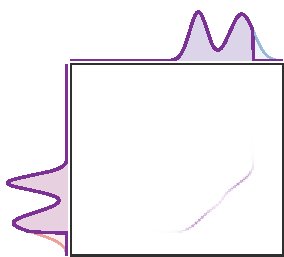
\includegraphics[width=.24\linewidth]{figures/partial-ot-active-mass/mass-090.pdf} &
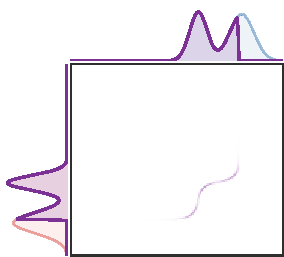
\includegraphics[width=.24\linewidth]{figures/partial-ot-active-mass/mass-065.pdf} &
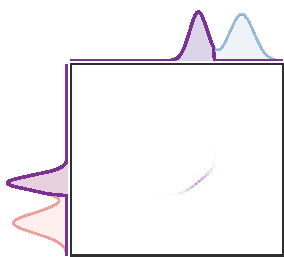
\includegraphics[width=.24\linewidth]{figures/partial-ot-active-mass/mass-042.pdf} &
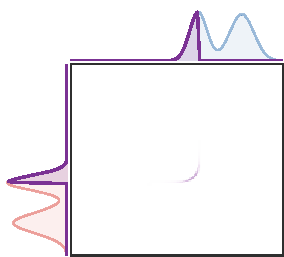
\includegraphics[width=.24\linewidth]{figures/partial-ot-active-mass/mass-022.pdf}
\end{tabular}
\caption{\emph{Partial optimal transport with prescribed transported mass between two shifted two-Gaussian mixtures.} The central image is the optimal subcoupling, with contrast normalized independently in each panel to keep the low-mass plans readable. The pale red and blue side curves are the original source and target densities, while the violet curves are the active truncated marginals $\pi_1$ and $\pi_2$. As $m$ decreases from left to right, only the closest facing portions remain matched and the remaining mass is left unmatched.}
\index{truncated marginal}% strictindex
\index{active mass}% strictindex
\index{partial transport}% strictindex
\label{fig:partial-ot-active-mass}
\end{figure}

The same mechanism becomes a geometric active-region selection in higher
dimension. Figure~\ref{fig:partial-ot-shape-active-mass} shows a two-dimensional
shape example: the partial plan selects the closest pieces of the two supports,
while leaving distant regions unmatched.

\begin{figure}[H]
\centering
\setlength{\tabcolsep}{2pt}
\begin{tabular}{@{}cccc@{}}
\small $m=0.82$ & \small $m=0.58$ & \small $m=0.36$ & \small $m=0.18$ \\[-.15em]
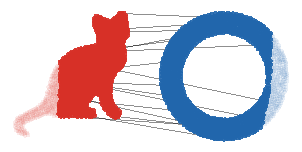
\includegraphics[width=.24\linewidth]{figures/partial-ot-shape-active-mass/mass-82.pdf} &
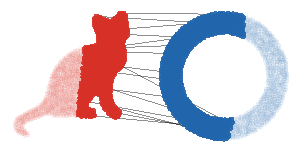
\includegraphics[width=.24\linewidth]{figures/partial-ot-shape-active-mass/mass-58.pdf} &
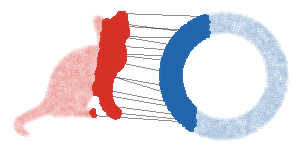
\includegraphics[width=.24\linewidth]{figures/partial-ot-shape-active-mass/mass-36.pdf} &
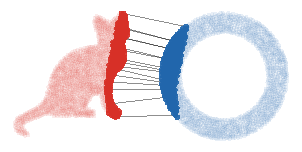
\includegraphics[width=.24\linewidth]{figures/partial-ot-shape-active-mass/mass-18.pdf}
\end{tabular}
\caption{\emph{Two-dimensional partial optimal transport between a red cat-shaped
indicator measure and a blue annulus indicator measure.} Both supports are
sampled by farthest-point sampling. In each panel, saturated points are the
active source and target marginals of the optimal partial plan, while pale
points are available mass left unmatched. Thin black segments show a
farthest-spaced subsample of transported source locations connected to the
dominant target selected by the plan. As the prescribed mass decreases, the
active regions contract to the nearest compatible pieces of the two shapes.}
\index{partial transport!active region}% strictindex
\label{fig:partial-ot-shape-active-mass}
\end{figure}


%%%%%%%%%%%%%%%%%%%%%%%%%%%%%%%%%%%%%%%%%%%%%%%%%%%%%%%%%%%%%%%%%%%%%%%%%%%
\section{Sliced Wasserstein Distances}
\index{Wasserstein!distance}% strictindex
\index{sliced Wasserstein!distance}% strictindex
\label{sec-sliced-wasserstein}

Sliced Wasserstein distances replace one high-dimensional comparison by an average of explicit one-dimensional optimal transport problems.

\paragraph{One-dimensional projections.}
Sliced Wasserstein trades exact high-dimensional geometry for many one-dimensional projections. The idea was originally proposed by Marc Bernot, and the first published work using this construction for Wasserstein barycenters and texture mixing is due to Rabin, Peyr\'e, Delon and Bernot~\cite{rabin-ssvm-11}. It is cheap, differentiable after sorting, and often effective in imaging and learning. For measures on $\RR^d$ and $\theta\in\Sphere^{d-1}$, let $P_\theta(x)=\dotp{\theta}{x}$ be the projection on direction $\theta$.
\index{one-dimensional!projection}% strictindex

\paragraph{Spherical averaging.}
The projected measures $(P_\theta)_\sharp\al$ and $(P_\theta)_\sharp\be$ live on the real line, where Wasserstein distances are computed by sorting or quantiles. Averaging these one-dimensional discrepancies over all directions gives the sliced distance.

\begin{defn}[Sliced Wasserstein distance]\label{def-sliced-wasserstein}
\index{projection direction}% strictindex
\index{spherical average}% strictindex
	Let $p\geq1$, let $\alpha,\beta\in\Pp_p(\RR^d)$, and let $\sigma$ be the uniform probability measure on the sphere $\Sphere^{d-1}$. The sliced $p$-Wasserstein distance is
	\eql{\label{eq-sliced-wasserstein}
		\SW_p(\al,\be)^p
		\eqdef
		\int_{\Sphere^{d-1}}
		\Wass_p\big((P_\theta)_\sharp\al,(P_\theta)_\sharp\be\big)^p
		\d\sigma(\theta).
	}
\end{defn}
Since each projected problem can be solved by sorting or quantiles, $\SW_p$ is much cheaper to approximate numerically than high-dimensional OT. It metrizes the same weak-plus-moment topology as $\Wass_p$, but its geometry is not bi-Lipschitz equivalent to $\Wass_p$ in high dimension~\cite{nadjahi2019asymptotic}.
\index{quantile!function}% strictindex
\index{probability measure}% strictindex

The family of all projected laws is itself a transform of measures.
\begin{defn}[Measure-valued Radon transform]\label{def-measure-radon-transform}
For $\al\in\Pp(\RR^d)$, define
\[
\mathfrak R\al(\theta)\eqdef(P_\theta)_\sharp\al,
\qquad \theta\in\Sphere^{d-1}.
\]
\end{defn}

\begin{rem}[Radon viewpoint]\label{rem-sliced-radon-viewpoint}
\index{measure-valued Radon transform}% strictindex
\index{projected measure}% strictindex
\index{Radon transform}% strictindex
\index{sliced Wasserstein!distance}% strictindex
	Slicing can also be understood as applying Definition~\ref{def-measure-radon-transform} before measuring discrepancy. Thus $\mathfrak R\al$ is a collection of one-dimensional projected measures indexed by directions. If $\al=\rho(x)\d x$ has a density, then $\mathfrak R\al(\theta)$ has density given by the classical Radon transform
	\[
		R\rho(\theta,s)
		=
		\int_{\{x:\dotp{\theta}{x}=s\}}\rho(x)\,\d\mathcal H^{d-1}(x).
	\]
	To make the metric meaning of ``pull-back'' explicit, equip Radon fields $h:\Sphere^{d-1}\to\Pp_p(\RR)$ with
\index{metric!pull-back}% strictindex
	\[
		d_{\mathrm{Rad},p}(h_0,h_1)
		\eqdef
		\left(
			\int_{\Sphere^{d-1}}
			\Wass_p\big(h_0(\theta),h_1(\theta)\big)^p
			\d\sigma(\theta)
		\right)^{1/p}.
	\]
	For any map $F:E\to(Y,d_Y)$, the pull-back of the metric $d_Y$ through $F$ is the function on $E\times E$ defined by
	\[
		(F^*d_Y)(x,x')\eqdef d_Y\big(F(x),F(x')\big).
	\]
	Consequently, \eqref{eq-sliced-wasserstein} reads
	\[
		\SW_p(\alpha,\beta)
		=
		d_{\mathrm{Rad},p}(\mathfrak R\alpha,\mathfrak R\beta)
		=
		(\mathfrak R^*d_{\mathrm{Rad},p})(\alpha,\beta).
	\]
	This is not the adjoint relation between the pull-back $T^\sharp g=g\circ T$ of a test function and the push-forward $T_\sharp$ of a measure discussed in Remark~\ref{rem-pullback-pushforward}, although both uses amount to precomposing an object by a map. Here one precomposes both arguments of a metric; each coordinate $\mathfrak R\alpha(\theta)=(P_\theta)_\sharp\alpha$ is itself a push-forward. A metric pull-back is generally only a pseudometric when $F$ is not injective. In the present setting, the full all-direction transform is injective on probability measures by the Cram\'er--Wold theorem~\cite{CramerWold1936}, which is why sliced Wasserstein separates measures. The warning is numerical and variational: finitely sampled Radon data are not injective, and independently constructed one-dimensional Radon data need not satisfy the range conditions of an actual image. This is precisely the issue behind sliced and Radon barycenter reconstructions discussed in Section~\ref{sec-barycenters} and illustrated in Figure~\ref{fig:sliced-radon-barycenter}.
\index{Cramer-Wold theorem}% strictindex
\index{Radon Wasserstein distance}% strictindex
\index{Radon range condition}% strictindex
\end{rem}

Figure~\ref{fig:sliced-wasserstein-projections} turns this Radon viewpoint into a concrete comparison: each planar density produces a family of one-dimensional projected laws, which can then be compared by ordinary one-dimensional Wasserstein distances.

\begin{figure}[H]
\centering
\setlength{\tabcolsep}{3pt}
\begin{tabular}{@{}cccc@{}}
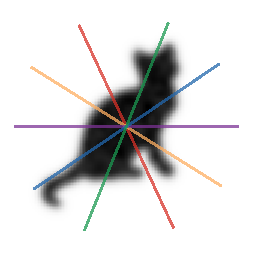
\includegraphics[width=.23\linewidth]{figures/sliced-wasserstein-projections/density-alpha.pdf} &
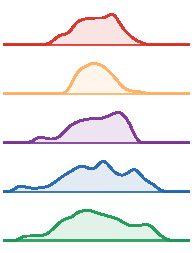
\includegraphics[width=.17\linewidth]{figures/sliced-wasserstein-projections/hist-alpha.pdf} &
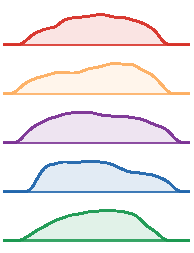
\includegraphics[width=.17\linewidth]{figures/sliced-wasserstein-projections/hist-beta.pdf} &
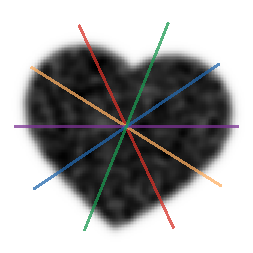
\includegraphics[width=.23\linewidth]{figures/sliced-wasserstein-projections/density-beta.pdf}
\\[-.1em]
\small source density & \small source slices & \small target slices & \small target density
\end{tabular}
\caption{\emph{Sliced Wasserstein projections between two planar densities.} The source and target are rendered as smoothed black-and-white density images obtained from dense farthest-point samples of two silhouettes. Five fixed directions are drawn on both densities. For each direction, the middle panels show smoothed one-dimensional density estimates of the projected measures $(P_\theta)_\sharp\alpha$ and $(P_\theta)_\sharp\beta$. Sliced OT averages one-dimensional Wasserstein discrepancies over many such directions, replacing a difficult planar comparison by a collection of sorted one-dimensional comparisons.}
\index{sliced Wasserstein!distance}% strictindex
\label{fig:sliced-wasserstein-projections}
\end{figure}

\begin{prop}[Metric properties of sliced Wasserstein]\label{prop-sliced-wasserstein-metric}
	For $p\geq1$, $\SW_p$ is a distance on $\Pp_p(\RR^d)$. Moreover, $\SW_p$ metrizes weak convergence together with convergence of the $p$th moment. Finally,
\index{weak!convergence}% strictindex
	\[
		\SW_p(\alpha,\beta)^p
		\leq
		\kappa_{d,p}\Wass_p(\alpha,\beta)^p,
		\qquad
		\kappa_{d,p}
		\eqdef
		\int_{\Sphere^{d-1}}|\theta_1|^p\d\sigma(\theta)
		=
		\frac{\Gamma(d/2)\Gamma((p+1)/2)}{\sqrt{\pi}\,\Gamma((d+p)/2)}.
	\]
	In particular, $\kappa_{d,2}=1/d$. Conversely, if $d\geq2$, $R>0$, and $\alpha,\beta\in\Pp_p(\RR^d)$ are supported in
	\(B_R\eqdef\enscond{x\in\RR^d}{\norm{x}\leq R}\), then there is a constant
	$C_{d,p}$ depending only on $d$ and $p$ such that Bonnotte's historical estimate reads
	\[
		\Wass_p(\alpha,\beta)^p
		\leq
		C_{d,p}R^{p-\frac{1}{d+1}}
		\SW_p(\alpha,\beta)^{\frac{1}{d+1}}.
	\]
	The sharp reverse estimate for $p=1$ also gives, for every $p\geq1$, constants $\widetilde C_{d,p},\widetilde c_{d,p}>0$ such that
	\[
		\Wass_p(\alpha,\beta)
		\leq
		\widetilde C_{d,p}
		R^{1-\frac{1}{pd}}
		\SW_p(\alpha,\beta)^{\frac{1}{pd}},
		\qquad\text{equivalently}\qquad
		\SW_p(\alpha,\beta)
		\geq
		\widetilde c_{d,p}R
		\left(\frac{\Wass_p(\alpha,\beta)}{R}\right)^{pd}.
	\]
	For $p=1$, the exponent $1/d$ in this last comparison is sharp.
\end{prop}

\begin{proof}
	Non-negativity and symmetry follow from the one-dimensional Wasserstein distance. For the triangle inequality, apply the triangle inequality of $\Wass_p$ for each direction $\theta$ and then Minkowski's inequality in $L^p(\Sphere^{d-1})$.
\index{Minkowski inequality}% strictindex
\index{triangle inequality}% strictindex
\index{Wasserstein!distance}% strictindex

	If $\SW_p(\alpha,\beta)=0$, then $(P_\theta)_\sharp\alpha=(P_\theta)_\sharp\beta$ for almost every direction. By continuity of characteristic functions this holds for all directions, and the Cram\'er--Wold theorem implies $\alpha=\beta$. This proves separation.

	Let $\pi$ be any coupling between $\alpha$ and $\beta$. Projecting $\pi$ gives an admissible coupling between the corresponding one-dimensional projections, hence
	\[
		\Wass_p\big((P_\theta)_\sharp\alpha,(P_\theta)_\sharp\beta\big)^p
		\leq
		\int_{\RR^d\times\RR^d}|\dotp{\theta}{x-y}|^p\d\pi(x,y).
	\]
	Rotational invariance of $\sigma$ gives
	\[
		\int_{\Sphere^{d-1}}|\dotp{\theta}{z}|^p\d\sigma(\theta)
		=
		\kappa_{d,p}\norm{z}^p.
	\]
	Integrating the first inequality in $\theta$ and optimizing over $\pi$ proves the stated direct comparison. The beta-integral formula for the first coordinate of a uniform point on the sphere gives the displayed value of $\kappa_{d,p}$; in particular, $\kappa_{d,2}=1/d$.

	To prove the topological statement, first suppose that $\Wass_p(\alpha_n,\alpha)\to0$. The inequality $\SW_p\leq\Wass_p$ immediately gives $\SW_p(\alpha_n,\alpha)\to0$. Conversely, suppose that $\SW_p(\alpha_n,\alpha)\to0$. The spherical identity
	\[
		\int_{\Sphere^{d-1}}\int_{\RR^d}|\langle\theta,x\rangle|^p\d\alpha_n(x)\d\sigma(\theta)
		=
		\kappa_{d,p}\int_{\RR^d}\|x\|^p\d\alpha_n(x),
		\qquad
		\kappa_{d,p}>0,
	\]
	and the triangle inequality in $L^p(\Sphere^{d-1}\times(0,1))$ show that the $p$th moments of $(\alpha_n)$ are uniformly bounded. Hence the sequence is tight. From every subsequence one can extract a further subsequence for which the projected $\Wass_p$ distances converge to zero for $\sigma$-a.e. $\theta$. Every weak limit therefore has the same one-dimensional projections as $\alpha$, so Cram\'er--Wold identifies it with $\alpha$. Thus $\alpha_n\rightharpoonup\alpha$. Finally, let $Q_{n,\theta}$ and $Q_\theta$ be the quantile functions of the projected measures. The one-dimensional quantile formula gives
	\[
		\SW_p(\alpha_n,\alpha)
		=
		\|Q_{n,\theta}-Q_\theta\|_{L^p(\Sphere^{d-1}\times(0,1))}.
	\]
	Hence the corresponding $L^p$ norms converge. By the spherical identity, their $p$th powers are respectively $\kappa_{d,p}\int\|x\|^p\d\alpha_n(x)$ and $\kappa_{d,p}\int\|x\|^p\d\alpha(x)$. Thus the $p$th moments converge. Weak convergence plus convergence of these moments is equivalent to convergence in $\Wass_p$.
	\index{tightness}% strictindex
	\index{one-dimensional!projection}% strictindex
	\index{weak!convergence}% strictindex

	\index{sliced Wasserstein!compact comparison}% strictindex
	\index{Radon structure}% strictindex
	The reverse estimates on compact sets are deeper and use the Radon structure of slices. Bonnotte's Lemma~5.1.4~\cite{bonnotte2013unidimensional} proves
	\[
		\Wass_1(\alpha,\beta)
		\leq
		C_dR^{\frac{d}{d+1}}\SW_1(\alpha,\beta)^{\frac{1}{d+1}}
	\]
	by mollifying a Kantorovich--Rubinstein test function, representing the regularized test through one-dimensional projections, bounding the resulting action by $\SW_1$, and optimizing the smoothing scale. On $B_R$,
	\[
		\Wass_p^p\leq(2R)^{p-1}\Wass_1,
		\qquad
		\SW_1\leq\SW_p,
	\]
	where the first inequality follows by evaluating the $p$-cost on a $\Wass_1$-optimal coupling, and the second follows from the monotonicity of one-dimensional Wasserstein distances and H\"older's inequality in $\theta$. These inequalities give Bonnotte's stated general-$p$ estimate. The sharper $p=1$ comparison theorem of Carlier, Figalli, M\'erigot and Wang~\cite{CarlierFigalliMerigotWang2025SlicedW1} replaces $1/(d+1)$ by the optimal exponent $1/d$. Combining it with the same two bounded-support inequalities gives
	\[
		\Wass_p^p
		\leq
		C_{d,p}R^{p-\frac1d}\SW_p^{\frac1d},
	\]
	which is equivalent to the final two-sided formulation in the statement. This supplies a lower bound on $\SW_p$ in terms of $\Wass_p$ for every $p$, but the asserted sharpness concerns only $p=1$.
\index{sliced Wasserstein!reverse bound}% strictindex
\end{proof}

The preceding estimates compare finite displacements. The infinitesimal
comparison is clearest along smooth Brenier perturbations: the usual
Wasserstein distance sees the full $L^2(\alpha)$ norm of the displacement,
whereas the sliced distance sees only its one-dimensional projections. The
same result also isolates the different behavior of finite atomic curves.

\begin{prop}[First-order comparison: strictness and atomic equality]\label{prop-sliced-first-order-tangent}
\index{Brenier!perturbation}% strictindex
\index{sliced tangent norm}% strictindex
\index{sliced Wasserstein!tangent norm}% strictindex
\index{metric!derivative}% strictindex
	Let $\alpha\in\Pp_2(\RR^d)$ be absolutely continuous, and let $\varphi\in C^2(\RR^d)$ be such that $\nabla\varphi\in L^2(\alpha;\RR^d)$ and $\nabla^2\varphi$ is bounded. For $\abs{t}$ small enough, set
	\[
		T_t(x)\eqdef x+t\nabla\varphi(x),
		\qquad
		\alpha_t\eqdef(T_t)_\sharp\alpha .
	\]
	Then $T_t$ is the quadratic Brenier map from $\alpha$ to $\alpha_t$ for $\abs{t}$ small enough, and
	\[
		\Wass_2(\alpha,\alpha_t)^2
		=
		t^2\int_{\RR^d}\norm{\nabla\varphi(x)}^2\d\alpha(x).
	\]
	Moreover,
	\[
		\SW_2(\alpha,\alpha_t)^2
		\leq
		\frac{t^2}{d}\int_{\RR^d}\norm{\nabla\varphi(x)}^2\d\alpha(x).
	\]
	The upper bound can be strict at order $t^2$. Indeed, let $d\geq2$, let
	$\alpha=\Gaussian(0,\Id)$, and take
	$\varphi(x)=\frac12 x^\top A x$ for a symmetric matrix $A$ that is not a
	scalar multiple of $\Id$. Then
	\[
		\lim_{t\to0}\frac{\SW_2(\alpha,\alpha_t)^2}{t^2}
		=
		\frac{\tr(A)^2+2\tr(A^2)}{d(d+2)}
		<
		\frac{\tr(A^2)}{d}
		=
		\frac1d\lim_{t\to0}\frac{\Wass_2(\alpha,\alpha_t)^2}{t^2}.
	\]
	Separately, equality holds at first order along every finite atomic curve
	with fixed weights. More precisely, let $a_i>0$ satisfy $\sum_i a_i=1$, let
	$x_1,\ldots,x_n$ be pairwise distinct, and let $v_i\in\RR^d$. If
	$\eta=\sum_{i=1}^n a_i\delta_{x_i}$ and
	$\eta_t=\sum_{i=1}^n a_i\delta_{x_i+t v_i}$, then
	\[
		\lim_{t\to0}\frac{\SW_2(\eta,\eta_t)^2}{t^2}
		=
		\frac1d\sum_{i=1}^n a_i\norm{v_i}^2
		=
		\frac1d\lim_{t\to0}\frac{\Wass_2(\eta,\eta_t)^2}{t^2}.
	\]
\end{prop}

\begin{proof}
	The map $T_t$ is the gradient of
	\[
		\psi_t(x)\eqdef \frac12\norm{x}^2+t\varphi(x).
	\]
	Since $\nabla^2\varphi$ is bounded, $\nabla^2\psi_t=\Id+t\nabla^2\varphi$ is positive semidefinite for $\abs{t}$ small enough. Hence $\psi_t$ is convex and $T_t=\nabla\psi_t$ is a Brenier map. Its graph is cyclically monotone, so the Brenier optimality criterion gives the optimality of $(\Id,T_t)_\sharp\alpha$, and
	\[
		\Wass_2(\alpha,\alpha_t)^2
		=
		\int\norm{x-T_t(x)}^2\d\alpha(x)
		=
		t^2\int\norm{\nabla\varphi(x)}^2\d\alpha(x).
	\]
	For a fixed direction $\theta$, the coupling
	\[
		\big(P_\theta,P_\theta\circ T_t\big)_\sharp\alpha
	\]
	is admissible between $(P_\theta)_\sharp\alpha$ and $(P_\theta)_\sharp\alpha_t$. Therefore
	\[
		\Wass_2\big((P_\theta)_\sharp\alpha,(P_\theta)_\sharp\alpha_t\big)^2
		\leq
		t^2\int\abs{\dotp{\theta}{\nabla\varphi(x)}}^2\d\alpha(x).
	\]
	Integrating over the sphere and using
	\[
		\int_{\Sphere^{d-1}}\abs{\dotp{\theta}{w}}^2\d\sigma(\theta)
		=
		\frac1d\norm{w}^2
	\]
	gives the sliced estimate.

	For the Gaussian example, $T_t=\Id+tA$ and, for every
	$\theta\in\Sphere^{d-1}$, the projected source and target are centered
	one-dimensional Gaussians with standard deviations $1$ and
	$\norm{(\Id+tA)\theta}$. Consequently,
	\[
		\lim_{t\to0}\frac{1}{t^2}
		\Wass_2\big((P_\theta)_\sharp\alpha,
		(P_\theta)_\sharp\alpha_t\big)^2
		=
		(\theta^\top A\theta)^2.
	\]
	The spherical fourth-moment identity gives
	\[
		\int_{\Sphere^{d-1}}(\theta^\top A\theta)^2\d\sigma(\theta)
		=
		\frac{\tr(A)^2+2\tr(A^2)}{d(d+2)}.
	\]
	On the other hand, the Brenier formula above gives
	$\Wass_2(\alpha,\alpha_t)^2=t^2\tr(A^2)$. The strict inequality follows
	from $\tr(A)^2<d\tr(A^2)$ when $A$ is symmetric and non-scalar.

	Finally, consider the atomic curve. For all sufficiently small $t$, the
	diagonal coupling between $x_i$ and $x_i+t v_i$ is optimal for $\Wass_2$.
	Indeed, writing $c_{ij}(t)=\norm{x_i-x_j-tv_j}^2$, the discrete dual
	potentials $f_i=0$ and $g_j=c_{jj}(t)$ are feasible for small $t$, because
	$c_{jj}(t)<c_{ij}(t)$ whenever $i\neq j$, and they certify the diagonal
	plan. Thus
	\[
		\Wass_2(\eta,\eta_t)^2
		=t^2\sum_{i=1}^n a_i\norm{v_i}^2.
	\]
	For every $\theta$ outside the finite union of great spheres
	$\{\dotp{\theta}{x_i-x_j}=0\}$, the projected atoms are distinct and their
	order is unchanged for sufficiently small $t$. The one-dimensional monotone
	coupling then pairs each projected atom with its perturbation, so
	\[
		\lim_{t\to0}\frac{1}{t^2}
		\Wass_2\big((P_\theta)_\sharp\eta,
		(P_\theta)_\sharp\eta_t\big)^2
		=
		\sum_{i=1}^n a_i\abs{\dotp{\theta}{v_i}}^2.
	\]
	The diagonal projected coupling provides the same expression as an
	integrable upper bound for every $t$. Dominated convergence and the spherical
	second-moment identity therefore give the asserted sliced limit.
\end{proof}

\paragraph{Intrinsic sliced length.}\label{par-sliced-intrinsic-length}
\index{sliced length metric}% strictindex
\index{intrinsic length metric}% strictindex
\index{sliced Wasserstein!length}% strictindex
\index{length metric}% strictindex
\index{path metric}% strictindex
In dimension one, $\SW_2=\Wass_2$. The geometry changes qualitatively for
$d\geq2$: $\SW_2$ is not a length metric~\cite{ParkSlepcev2023SlicedGeometry}.
Its intrinsic, or path, metric is
\begin{equation}\label{eq-intrinsic-sliced-length}
	\ell_{\SW_2}(\alpha,\beta)
	\eqdef
	\inf_{\substack{\gamma_0=\alpha,\ \gamma_1=\beta\\
		\gamma\ \text{$\SW_2$-absolutely continuous}}}
	\int_0^1 \abs{\dot\gamma_t}_{\SW_2}\,\d t,
\end{equation}
where $\abs{\dot\gamma_t}_{\SW_2}$ is the metric derivative. Park and
Slep\v{c}ev prove that the infimum is attained, so
$(\Pp_2(\RR^d),\ell_{\SW_2})$ is a geodesic space. Every path length dominates
the distance between its endpoints, while
Proposition~\ref{prop-sliced-wasserstein-metric} bounds the $\SW_2$-length of a
$\Wass_2$-geodesic. Consequently,
\[
	\SW_2\leq\ell_{\SW_2}\leq d^{-1/2}\Wass_2.
\]

Neither inequality identifies the intrinsic geometry with a rescaled
Wasserstein geometry. Proposition~\ref{prop-sliced-first-order-tangent} shows
that the sliced metric derivative equals $d^{-1/2}$ times the Wasserstein
metric derivative along finite atomic curves with fixed weights. By contrast,
the Gaussian deformation in the same proposition is strictly slower for
$\SW_2$. The sliced speed along
$s\mapsto(\Id+sA)_\sharp\Gaussian(0,\Id)$ depends continuously on $s$, so this
strictness persists on a short interval. Integrating along that
$\Wass_2$-geodesic gives, for every sufficiently small $t\neq0$,
\[
	\ell_{\SW_2}(\alpha,\alpha_t)
	<d^{-1/2}\Wass_2(\alpha,\alpha_t).
\]

There is, more strongly, no reverse comparison by a constant depending only on
the dimension. Example~3.2 of Park and Slep\v{c}ev considers two nearby
parallel line segments moving in opposite directions. Most projected motions
cancel after slicing: for every $\delta>0$, the construction produces a
compactly supported, atomless curve $(\alpha_t^\delta)_t$ such that, for small
$t\geq0$,
\[
	\abs{\dot\alpha_t^\delta}_{\Wass_2}=1,
	\qquad
	\abs{\dot\alpha_t^\delta}_{\SW_2}\leq C_d(t+\delta).
\]
Since the first identity gives
$\Wass_2(\alpha_0^\delta,\alpha_h^\delta)=h+o(h)$, while the second gives
$\ell_{\SW_2}(\alpha_0^\delta,\alpha_h^\delta)
\leq C_d(\delta h+h^2/2)$, one obtains
\[
	\limsup_{h\downarrow0}
	\frac{\ell_{\SW_2}(\alpha_0^\delta,\alpha_h^\delta)}
	     {\Wass_2(\alpha_0^\delta,\alpha_h^\delta)}
	\leq C_d\delta.
\]
Letting $\delta\to0$ yields
\begin{equation}\label{eq-no-lower-comparison-sliced-length}
	\inf_{\substack{\alpha,\beta\in\Pp_2(\RR^d)\\\alpha\neq\beta}}
	\frac{\ell_{\SW_2}(\alpha,\beta)}{\Wass_2(\alpha,\beta)}=0.
\end{equation}
Thus $\ell_{\SW_2}$ and $\Wass_2$ are not globally bi-Lipschitz equivalent,
even after inserting the factor $d^{-1/2}$.

The atomic equality is nevertheless stable in its natural regime. If $\eta$
is a fixed finite atomic measure with positive masses and separated atoms,
Theorem~5.5 of Park and Slep\v{c}ev gives
\[
	\frac{\SW_2(\eta,\beta)}{\Wass_2(\eta,\beta)}
	\longrightarrow\frac1{\sqrt d},
	\qquad
	\frac{\ell_{\SW_2}(\eta,\beta)}{\Wass_2(\eta,\beta)}
	\longrightarrow\frac1{\sqrt d}
	\quad\text{as }\Wass_\infty(\eta,\beta)\to0,
\]
along $\beta\neq\eta$; see~\eqref{eq-wass-infty}. By contrast, under suitable
common-support and density bounds in the diffuse regime, their Theorem~5.2
shows that both $\SW_2$ and $\ell_{\SW_2}$ are locally equivalent to the
negative Sobolev norm $\dot H^{-(d+1)/2}$, whereas the infinitesimal geometry
of $\Wass_2$ around a positive density is of $\dot H^{-1}$ type. These results
settle the comparison: the intrinsic sliced metric agrees asymptotically with
$d^{-1/2}\Wass_2$ near finite atomic measures, but it is a genuinely different
metric globally and around diffuse measures.

\begin{rem}[Hilbert embedding for $\SW_2$]\label{rem-sliced-hilbert-embedding}
\index{Hilbert!embedding}% strictindex
	In one dimension, $\Wass_2$ is the $L^2(0,1)$ distance between quantile functions. Hence
\index{quantile!function}% strictindex
	\[
		\SW_2(\alpha,\beta)^2
		=
		\int_{\Sphere^{d-1}}\int_0^1
		\abs{F_{\theta,\alpha}^{-1}(u)-F_{\theta,\beta}^{-1}(u)}^2
		\d u\d\sigma(\theta),
	\]
	where $F_{\theta,\alpha}^{-1}$ is the quantile of $(P_\theta)_\sharp\alpha$. Thus $\SW_2$ is a Hilbertian distance after embedding each measure into its field of projected quantiles. Consequently, $\exp(-\gamma\SW_2^2)$ is a positive definite kernel on probability measures for every $\gamma>0$.
\index{quantile!function}% strictindex
\index{probability measure}% strictindex
\index{kernel!positive definite}% strictindex
	The compact reverse estimates in Proposition~\ref{prop-sliced-wasserstein-metric} explain why sliced distances metrize the same topology on bounded sets, while the dimension-dependent powers prevent a dimension-free bi-Lipschitz comparison with $\Wass_p$.
\end{rem}

\paragraph{Sliced Wasserstein between Gaussians.}
\index{sliced Wasserstein!Gaussian}% strictindex
\index{Gaussian!sliced Wasserstein}% strictindex

Gaussian projections remain Gaussian, so quadratic sliced transport reduces
to the one-dimensional Gaussian formula in every direction. This gives an
exact angular representation and makes its relation with the Bures covariance
geometry explicit.

\begin{prop}[Sliced Wasserstein between Gaussians]\label{prop-sliced-gaussian}
	Let
	\(
		\alpha=\Gaussian(m_\alpha,\Sigma_\alpha)
	\)
	and
	\(
		\beta=\Gaussian(m_\beta,\Sigma_\beta)
	\)
	on $\RR^d$, where the covariance matrices are positive semidefinite. Then
	\begin{align}
		\SW_2(\alpha,\beta)^2
		&=
		\frac{\norm{m_\alpha-m_\beta}^2}{d}
		+
		\int_{\Sphere^{d-1}}
		\pa{
			\sqrt{\transp{\theta}\Sigma_\alpha\theta}
			-
			\sqrt{\transp{\theta}\Sigma_\beta\theta}
		}^2
		\d\sigma(\theta) \label{eq-sliced-gaussian}\\
		&=
		\frac{
			\norm{m_\alpha-m_\beta}^2
			+\tr(\Sigma_\alpha)+\tr(\Sigma_\beta)
		}{d}
		-2\int_{\Sphere^{d-1}}
		\sqrt{
			(\transp{\theta}\Sigma_\alpha\theta)
			(\transp{\theta}\Sigma_\beta\theta)
		}
		\d\sigma(\theta). \nonumber
	\end{align}
	Moreover,
	\begin{equation}\label{eq-sliced-gaussian-fidelity}
		\int_{\Sphere^{d-1}}
		\sqrt{
			(\transp{\theta}\Sigma_\alpha\theta)
			(\transp{\theta}\Sigma_\beta\theta)
		}
		\d\sigma(\theta)
		\geq
		\frac1d
		\tr\!\left[
			\bigl(
				\Sigma_\alpha^{1/2}
				\Sigma_\beta
				\Sigma_\alpha^{1/2}
			\bigr)^{1/2}
		\right],
	\end{equation}
	and hence
	\[
		\SW_2(\alpha,\beta)^2
		\leq
		\frac1d\Wass_2(\alpha,\beta)^2.
	\]
	If both covariances are positive definite, equality holds if and only if
	they are proportional. More generally, if
	\[
		\Sigma_\alpha=s^2\Sigma,
		\qquad
		\Sigma_\beta=t^2\Sigma
	\]
	for some positive semidefinite $\Sigma$ and $s,t\geq0$, then
	\begin{equation}\label{eq-sliced-gaussian-proportional}
		\SW_2(\alpha,\beta)^2
		=
		\frac{1}{d}\Wass_2(\alpha,\beta)^2
		=
		\frac{
			\norm{m_\alpha-m_\beta}^2
			+(s-t)^2\tr(\Sigma)
		}{d}.
	\end{equation}
\end{prop}
\begin{proof}
	For every $\theta\in\Sphere^{d-1}$,
	\[
		(P_\theta)_\sharp\alpha
		=
		\Gaussian\bigl(\transp{\theta}m_\alpha,
		\transp{\theta}\Sigma_\alpha\theta\bigr),
	\]
	and similarly for $\beta$. The one-dimensional Gaussian formula therefore
	gives the integrand in~\eqref{eq-sliced-gaussian}. Expanding the square and
	using
	\(
		\int_{\Sphere^{d-1}}\theta\transp{\theta}\,\d\sigma(\theta)=\Id/d
	\)
	gives the second expression.

	First suppose that both covariances are positive definite and let $A$ be
	the Bures transport matrix~\eqref{eq-bures-map}, so that
	$A\Sigma_\alpha A=\Sigma_\beta$. Cauchy--Schwarz for the inner product
	$\dotp{x}{y}_{\Sigma_\alpha}=\transp{x}\Sigma_\alpha y$ gives, for every
	$\theta$,
	\[
		\transp{\theta}\Sigma_\alpha A\theta
		\leq
		\sqrt{
			(\transp{\theta}\Sigma_\alpha\theta)
			(\transp{\theta}A\Sigma_\alpha A\theta)
		}
		=
		\sqrt{
			(\transp{\theta}\Sigma_\alpha\theta)
			(\transp{\theta}\Sigma_\beta\theta)
		}.
	\]
	Integrating and using the spherical second-moment identity yields
	\[
		\int_{\Sphere^{d-1}}
		\sqrt{
			(\transp{\theta}\Sigma_\alpha\theta)
			(\transp{\theta}\Sigma_\beta\theta)
		}
		\d\sigma(\theta)
		\geq
		\frac{\tr(\Sigma_\alpha A)}{d}
		=
		\frac1d
		\tr\!\left[
			\bigl(
				\Sigma_\alpha^{1/2}
				\Sigma_\beta
				\Sigma_\alpha^{1/2}
			\bigr)^{1/2}
		\right].
	\]
	The general positive-semidefinite case follows by continuity. Combining
	this bound with~\eqref{eq-sliced-gaussian} and the Bures
	formula~\eqref{eq-dist-gauss} proves the comparison.

	In the positive-definite case, equality in the integral requires equality
	in Cauchy--Schwarz for almost every $\theta$. By continuity, this holds for
	every $\theta$, so $A\theta$ is collinear with $\theta$ for every
	$\theta$. A linear map with this property is a scalar multiple of the
	identity; hence $A=r\Id$ and $\Sigma_\beta=r^2\Sigma_\alpha$. The converse
	is immediate. Finally, for
	$\Sigma_\alpha=s^2\Sigma$ and $\Sigma_\beta=t^2\Sigma$, the covariance
	integrand in~\eqref{eq-sliced-gaussian} is
	$(s-t)^2\transp{\theta}\Sigma\theta$. Averaging it gives
	$(s-t)^2\tr(\Sigma)/d$, and the Bures formula gives the same covariance
	term before division by $d$.
\end{proof}

Formula~\eqref{eq-sliced-gaussian} is exact, but for generic anisotropic
covariances its spherical integral has no Bures-like matrix-square-root
simplification and is evaluated by angular quadrature or Monte Carlo. The
comparison in the proposition is the Gaussian specialization of
Proposition~\ref{prop-sliced-wasserstein-metric}. Its normalization matters:
for $d>1$ and $\alpha\neq\beta$, $\SW_2$ is necessarily strictly smaller than
$\Wass_2$, whereas the two distances coincide in dimension one.

Two isotropic covariances lie on the same ray: if
$\Sigma_\alpha=s^2\Id$ and $\Sigma_\beta=t^2\Id$, then
\[
	\SW_2(\alpha,\beta)^2
	=
	\frac{\norm{m_\alpha-m_\beta}^2}{d}
	+(s-t)^2
	=
	\frac1d\Wass_2(\alpha,\beta)^2.
\]
One isotropic covariance does not suffice. If
$\Sigma_\alpha=s^2\Id$, with $s>0$, and $\Sigma_\beta$ is arbitrary, then
\[
	\SW_2(\alpha,\beta)^2
	=
	\frac{\norm{m_\alpha-m_\beta}^2}{d}
	+s^2+\frac{\tr(\Sigma_\beta)}{d}
	-2s\int_{\Sphere^{d-1}}
	\sqrt{\transp{\theta}\Sigma_\beta\theta}\,\d\sigma(\theta).
\]
If $(\lambda_i)_{i=1}^d$ are the eigenvalues of $\Sigma_\beta$, concavity of
the square root gives, in an associated eigenbasis,
\[
	\sqrt{\transp{\theta}\Sigma_\beta\theta}
	=
	\sqrt{\sum_i\lambda_i\theta_i^2}
	\geq
	\sum_i\sqrt{\lambda_i}\,\theta_i^2.
\]
After integration,
\(
	\int\sqrt{\transp{\theta}\Sigma_\beta\theta}\,\d\sigma(\theta)
	\geq d^{-1}\tr(\Sigma_\beta^{1/2})
\),
with equality precisely when $\Sigma_\beta$ is isotropic. Thus an anisotropic
$\Sigma_\beta$ gives the strict inequality
$\SW_2^2<\Wass_2^2/d$.

Rank-one covariances make the loss of orientation information particularly
transparent. If
$\Sigma_\alpha=a^2u\transp{u}$ and
$\Sigma_\beta=b^2v\transp{v}$, where $u,v$ are unit vectors and
$\chi=\abs{\dotp{u}{v}}$, then
\begin{align*}
	\SW_2(\alpha,\beta)^2
	&=
	\frac1d\left[
		\norm{m_\alpha-m_\beta}^2+a^2+b^2
		-\frac{4ab}{\pi}
		\pa{\sqrt{1-\chi^2}+\chi\arcsin(\chi)}
	\right],\\
	\Wass_2(\alpha,\beta)^2
	&=
	\norm{m_\alpha-m_\beta}^2+a^2+b^2-2ab\chi.
\end{align*}
Indeed, by rotational invariance one may take
$u=e_1$ and $v=\chi e_1+\sqrt{1-\chi^2}\,e_2$. Writing
$(\theta_1,\theta_2)=R(\cos\varphi,\sin\varphi)$, where $\varphi$ is uniform
and $\EE(R^2)=2/d$, an elementary angular integration gives
\[
	\int_{\Sphere^{d-1}}
	\abs{\dotp{u}{\theta}}\abs{\dotp{v}{\theta}}\,\d\sigma(\theta)
	=
	\frac{2}{\pi d}
	\pa{\sqrt{1-\chi^2}+\chi\arcsin(\chi)}.
\]
Aligned rank-one covariances saturate~\eqref{eq-sliced-gaussian-proportional},
whereas centered, orthogonal, equal-scale covariances satisfy
$\SW_2=\sqrt{1-2/\pi}\,\Wass_2/\sqrt d$. Thus sliced transport retains the
relative angle, but attenuates it through an angular average rather than the
linear Bures factor $\chi$. The associated Gaussian sliced-Wasserstein flow is
revisited in Proposition~\ref{prop-centered-gaussian-covariance-catalogue}.

\paragraph{$L^q$-sliced, max-sliced and subspace variants.}
\index{sliced Wasserstein!directional aggregation}% strictindex
\index{sliced Wasserstein!max}% strictindex
\index{subspace-sliced Wasserstein}% strictindex

The exponent used to aggregate projection directions need not coincide with the
transport exponent. A second exponent $q$ controls this aggregation: finite
$q$ pools information from many directions, whereas $q=\infty$ retains only
the most discriminating one. Independently, replacing lines by
$k$-dimensional subspaces preserves more correlations at the price of solving
higher-dimensional projected OT problems. These two choices fit into one
family.

\begin{defn}[$L^q$-sliced and subspace-sliced Wasserstein]\label{def-sliced-variants}
\index{sliced Wasserstein!distance}% strictindex
\index{Stiefel manifold}% strictindex
	Let $p\in[1,\infty)$, $q\in[1,\infty]$, and $1\leq k\leq d$. Denote by
	\[
		\mathrm{St}(d,k)
		\eqdef
		\enscond{U\in\RR^{d\times k}}{\transp{U}U=\Id_k}
	\]
	the Stiefel manifold, equipped with its normalized invariant probability
	measure $\sigma_{d,k}$. For $q<\infty$, define
	\begin{equation}\label{eq-lq-subspace-sliced}
		\SW_{p,q,k}(\alpha,\beta)
		\eqdef
		\left(
			\int_{\mathrm{St}(d,k)}
			\Wass_p\big((\transp{U})_\sharp\alpha,
			              (\transp{U})_\sharp\beta\big)^q
			\d\sigma_{d,k}(U)
		\right)^{1/q},
	\end{equation}
	and extend the definition to $q=\infty$ by
	\[
		\SW_{p,\infty,k}(\alpha,\beta)
		\eqdef
		\sup_{U\in\mathrm{St}(d,k)}
		\Wass_p\big((\transp{U})_\sharp\alpha,
		              (\transp{U})_\sharp\beta\big).
	\]
	The supremum is attained because the Stiefel manifold is compact and the
	projected Wasserstein distance depends continuously on $U$. Moreover, the
	integrand is unchanged under $U\mapsto UQ$ for $Q\in\mathrm O(k)$, because
	$Q^\top$ is an isometry of $\RR^k$. Thus the construction depends only on the
	subspace spanned by the columns of $U$: the Stiefel manifold is a convenient
	parametrization of the corresponding Grassmann manifold.
	\index{Grassmann manifold}% strictindex
	We use the abbreviations
	\[
		\SW_{p,q}\eqdef\SW_{p,q,1},
		\qquad
		\SW_p=\SW_{p,p},
		\qquad
		\MaxSW_{p,k}\eqdef\SW_{p,\infty,k},
		\qquad
		\MaxSW_p=\SW_{p,\infty}.
	\]
	Thus $k=1$ gives line-based slicing, $q=\infty$ gives max-slicing,
	and $k=d$ gives $\SW_{p,q,d}=\Wass_p$ for every $q$. Quadratic max-slicing is useful
	when only a small set of directions carries the discrepancy, for instance in
	generative modeling~\cite{deshpande2019maxsliced}. For $p=2$, the $k$-dimensional
	max-sliced case is the projection-robust Wasserstein distance, which is related to the
	subspace-robust distances studied later in
	Section~\ref{sec-spectral-subspace-wasserstein}~\cite{paty2019subspace}.
\index{generative model}% strictindex
\index{projection-robust Wasserstein}% strictindex
\end{defn}

Metricity and the direct comparison with $\Wass_p$ carry over from ordinary
slicing. The topological statement requires slightly more care when $q<p$:
although an abstract $L^q$ norm need not control an $L^p$ norm, projected
Wasserstein profiles have enough continuity and moment control to rule out
concentration in a vanishing set of subspaces. The next proposition records
these facts and separates the roles of $p$, $q$, and $k$.

\begin{prop}[Basic bounds for sliced variants]\label{prop-sliced-variant-bounds}
\index{sliced Wasserstein!distance}% strictindex
\index{subspace!projection}% strictindex
	Let $p\in[1,\infty)$, $1\leq q\leq r\leq\infty$, and
	$1\leq k\leq \ell\leq d$. Each $\SW_{p,q,k}$ is a finite distance on
	$\Pp_p(\RR^d)$ and metrizes the same topology as $\Wass_p$. For every
	$\alpha,\beta\in\Pp_p(\RR^d)$,
	\begin{align}
		\SW_{p,q,k}(\alpha,\beta)
		&\leq
		\SW_{p,r,k}(\alpha,\beta)
		\leq
		\Wass_p(\alpha,\beta),
		\label{eq-lq-sliced-monotonicity}\\
		\SW_{p,q,k}(\alpha,\beta)
		&\leq
		\SW_{p,q,\ell}(\alpha,\beta)
		\leq
		\Wass_p(\alpha,\beta).
		\label{eq-subspace-dimension-monotonicity}
	\end{align}
	For a unit vector $e\in\Sphere^{d-1}$, set
	\[
		\kappa_{d,k,p}
		\eqdef
		\int_{\mathrm{St}(d,k)}\norm{\transp{U}e}^p\d\sigma_{d,k}(U)
		=
		\frac{\Gamma(d/2)\Gamma((k+p)/2)}
		     {\Gamma(k/2)\Gamma((d+p)/2)}.
	\]
	This constant is independent of $e$, satisfies $\kappa_{d,d,p}=1$ and
	$\kappa_{d,1,p}=\kappa_{d,p}$ from
	Proposition~\ref{prop-sliced-wasserstein-metric}, and gives the sharper bounds
	\begin{equation}\label{eq-lq-subspace-sliced-upper-bound}
		\SW_{p,q,k}(\alpha,\beta)
		\leq
		\begin{cases}
			\kappa_{d,k,p}^{1/p}\Wass_p(\alpha,\beta), & 1\leq q\leq p,\\
			\kappa_{d,k,p}^{1/q}\Wass_p(\alpha,\beta), & p\leq q<\infty,\\
			\Wass_p(\alpha,\beta), & q=\infty.
		\end{cases}
	\end{equation}
	Moreover,
	\begin{equation}\label{eq-subspace-sliced-lower-bound}
		\SW_p(\alpha,\beta)
		\leq
		\SW_{p,p,k}(\alpha,\beta)
		\leq
		\kappa_{d,k,p}^{1/p}\Wass_p(\alpha,\beta).
	\end{equation}
	In particular, $\kappa_{d,k,2}=k/d$ and
	$\SW_{2,2,k}^2\leq(k/d)\Wass_2^2$. If $q\geq p$, the compact-support reverse
	estimates in Proposition~\ref{prop-sliced-wasserstein-metric} remain valid
	with $\SW_{p,q,k}$ in place of $\SW_p$.
\end{prop}

\begin{proof}
	Write
	$D_U(\alpha,\beta)\eqdef
	\Wass_p((\transp{U})_\sharp\alpha,(\transp{U})_\sharp\beta)$.
	Non-negativity and symmetry are inherited from $\Wass_p$.
	Minkowski's inequality in $L^q(\sigma_{d,k})$, or the supremum triangle
	inequality when $q=\infty$, proves the triangle inequality. The reverse
	triangle inequality for $\Wass_p$ shows that $U\mapsto D_U(\alpha,\beta)$ is
	continuous. Indeed, for $U_n\to U$,
	\[
		\Wass_p\big((\transp{U_n})_\sharp\alpha,(\transp{U})_\sharp\alpha\big)
		\leq
		\norm{U_n-U}_{\mathrm{op}}
		\left(\int\norm{x}^p\d\alpha(x)\right)^{1/p},
	\]
	and likewise for $\beta$. If $\SW_{p,q,k}(\alpha,\beta)=0$, then $D_U=0$ for
	all $U$: this is immediate for $q=\infty$, while for finite $q$ it follows
	from continuity and the full support of $\sigma_{d,k}$. For any
	$\theta\in\Sphere^{d-1}$, choose a frame $U$ whose first column is $\theta$.
	Equality of the two $k$-dimensional projected measures then implies equality
	of their first-coordinate marginals, hence
	$(P_\theta)_\sharp\alpha=(P_\theta)_\sharp\beta$. The Cram\'er--Wold theorem
	gives $\alpha=\beta$, proving separation.

	Every $U^\top$ is $1$-Lipschitz, so $D_U\leq\Wass_p(\alpha,\beta)$.
	Monotonicity of $L^q$ norms on a probability space proves
	\eqref{eq-lq-sliced-monotonicity}. To compare projection dimensions, let
	$V\in\mathrm{St}(d,\ell)$ and $R\in\mathrm{St}(\ell,k)$. Since
	$(VR)^\top=R^\top V^\top$ and $R^\top$ is $1$-Lipschitz,
	$D_{VR}(\alpha,\beta)\leq D_V(\alpha,\beta)$. Under the product of the
	invariant measures, $VR$ is uniformly distributed on $\mathrm{St}(d,k)$.
	Integration proves~\eqref{eq-subspace-dimension-monotonicity} for finite $q$;
	for $q=\infty$, extend each $k$-frame to an $\ell$-frame and use the same
	contraction.

	For the sharper constants, let $\pi\in\Gamma(\alpha,\beta)$. Then
	\[
		D_U(\alpha,\beta)^p
		\leq
		\int\norm{\transp{U}(x-y)}^p\d\pi(x,y).
	\]
	Integration in $U$, followed by minimization in $\pi$, gives
	$\norm{D_\cdot}_{L^p(\sigma_{d,k})}^p
	\leq\kappa_{d,k,p}\Wass_p(\alpha,\beta)^p$. If $q\leq p$, use
	$\norm{D_\cdot}_{L^q}\leq\norm{D_\cdot}_{L^p}$. If $p\leq q<\infty$, use
	$D_U\leq\Wass_p$ to obtain
	\[
		\int D_U^q\d\sigma_{d,k}(U)
		\leq
		\Wass_p(\alpha,\beta)^{q-p}
		\int D_U^p\d\sigma_{d,k}(U).
	\]
	This proves~\eqref{eq-lq-subspace-sliced-upper-bound}. The beta-integral for
	the $p$th power of the length of a random $k$-dimensional projection gives
	the displayed formula for $\kappa_{d,k,p}$.

	Finally, let $\omega\in\Sphere^{k-1}$. Since
	$P_{U\omega}=P_\omega\circ U^\top$, projection contraction gives
	\[
		\Wass_p\big((P_{U\omega})_\sharp\alpha,
		              (P_{U\omega})_\sharp\beta\big)
		\leq D_U(\alpha,\beta).
	\]
	Averaging its $p$th power first over $\omega$ and then over $U$ makes
	$U\omega$ uniform on $\Sphere^{d-1}$ and proves the first inequality
	in~\eqref{eq-subspace-sliced-lower-bound}. For $q\geq p$,
	\eqref{eq-lq-sliced-monotonicity} gives
	$\SW_p\leq\SW_{p,p,k}\leq\SW_{p,q,k}$, which transfers the stated reverse
	estimates.

	It remains to prove the topological assertion. For
	$\eta\in\Pp_p(\RR^d)$, set
	$M_p(\eta)\eqdef(\int\norm{x}^p\d\eta(x))^{1/p}$. Since the only coupling
	between $(U^\top)_\sharp\eta$ and $\delta_0$ sends every point to the origin,
	\[
		D_U(\eta,\delta_0)^p
		=
		\int\norm{U^\top x}^p\d\eta(x),
		\qquad
		\int D_U(\eta,\delta_0)^p\d\sigma_{d,k}(U)
		=
		\kappa_{d,k,p}M_p(\eta)^p.
	\]
	Also $D_U(\eta,\delta_0)\leq M_p(\eta)$. Consequently,
	\begin{equation}\label{eq-lq-sliced-radial-moment}
		\SW_{p,q,k}(\eta,\delta_0)
		\geq
		\begin{cases}
			\kappa_{d,k,p}^{1/q}M_p(\eta), & 1\leq q\leq p,\\
			\kappa_{d,k,p}^{1/p}M_p(\eta), & p\leq q\leq\infty.
		\end{cases}
	\end{equation}
	Indeed, the second line follows from monotonicity of $L^q$ norms. For
	$q\leq p$ and $M_p(\eta)>0$, the pointwise bound
	$D_U\leq M_p(\eta)$ gives
	$D_U^q\geq M_p(\eta)^{q-p}D_U^p$; the zero-moment case is immediate.

	Suppose now that $\SW_{p,q,k}(\alpha_n,\alpha)\to0$. The triangle inequality
	and~\eqref{eq-lq-sliced-radial-moment} imply
	$\sup_n M_p(\alpha_n)<\infty$. Write
	$D_{n,U}\eqdef D_U(\alpha_n,\alpha)$. The reverse triangle inequality and
	the coupling of each point with itself give
	\[
		\abs{D_{n,U}-D_{n,V}}
		\leq
		\norm{U-V}_{\mathrm{op}}
		\big(M_p(\alpha_n)+M_p(\alpha)\big),
	\]
	so $(D_{n,\cdot})_n$ is equicontinuous on the compact Stiefel manifold. For
	$q<\infty$, equicontinuity and the full support of $\sigma_{d,k}$ upgrade
	$\norm{D_{n,\cdot}}_{L^q}\to0$ to $\norm{D_{n,\cdot}}_{L^\infty}\to0$;
	for $q=\infty$ this is immediate. Given $\theta\in\Sphere^{d-1}$, choose a
	frame $U$ whose first column is $\theta$. Projection contraction then yields
	\[
		\Wass_p\big((P_\theta)_\sharp\alpha_n,(P_\theta)_\sharp\alpha\big)
		\leq D_{n,U},
	\]
	uniformly in $\theta$. Hence $\SW_p(\alpha_n,\alpha)\to0$, and
	Proposition~\ref{prop-sliced-wasserstein-metric} gives
	$\Wass_p(\alpha_n,\alpha)\to0$. The converse follows directly from
	$\SW_{p,q,k}\leq\Wass_p$.
\end{proof}

\paragraph{Min-SW lifted transport plans.}
\index{Min-SW}% strictindex
\index{plan!lifted}% strictindex

The preceding constructions compare projected measures. Min-SW uses a projection differently: it lifts the one-dimensional monotone coupling back to the ambient space and retains the lift with the smallest quadratic cost. Consider equal-weight empirical measures
$\alpha=n^{-1}\sum_i\delta_{x_i}$ and $\beta=n^{-1}\sum_i\delta_{y_i}$.
For a direction $\theta$ along which both projected point families have distinct coordinates, let $\sigma_\theta,\tau_\theta\in\mathfrak S_n$ be their sorting permutations,
\index{empirical!measure}% strictindex
\index{monotone!matching}% strictindex
\[
	\dotp{x_{\sigma_\theta(1)}}{\theta}<\cdots<
	\dotp{x_{\sigma_\theta(n)}}{\theta},
	\qquad
	\dotp{y_{\tau_\theta(1)}}{\theta}<\cdots<
	\dotp{y_{\tau_\theta(n)}}{\theta}.
\]
Lifting the one-dimensional monotone matching gives
\begin{equation}\label{eq-min-sw-empirical-plan}
	\pi_\theta
	=
	\frac1n\sum_{i=1}^n
	\delta_{(x_{\sigma_\theta(i)},y_{\tau_\theta(i)})}
	\in\Couplings(\alpha,\beta).
\end{equation}
The cost of~\eqref{eq-min-sw-empirical-plan} is an upper bound on $\Wass_2(\alpha,\beta)^2$, and Min-SW minimizes this upper bound over $\theta$. This inexpensive feasible-plan construction was introduced by Mahey, Chapel, Gasso, Bonet and Courty~\cite{MaheyChapelGassoBonetCourty2023MinSW}.

Projected ties make the extension beyond this generic empirical setting less immediate. At a tie, the sorting permutations are not unique. Breaking ties by labels is not invariant under a relabeling of the atoms, while a lexicographic rule depends on an auxiliary coordinate system; both choices can be discontinuous under perturbations. For a non-discrete measure, a projection fiber may moreover carry an entire conditional distribution, so there are no labels to sort. Tanguy, Chapel and Delon~\cite{TanguyChapelDelon2025SlicedTransportPlans} avoid arbitrary tie breaking by optimizing over all compatible lifts. Set
\[
	\alpha_\theta=(P_\theta)_\sharp\alpha,
	\qquad
	\beta_\theta=(P_\theta)_\sharp\beta,
\]
and let
\[
	\varpi_\theta
	=
	(q_{\alpha_\theta},q_{\beta_\theta})_\sharp
	\mathrm{Leb}_{[0,1]}
\]
be their canonical monotone coupling, as in Theorem~\ref{prop-1d-kantorovich-quantile-coupling}. Define
\begin{defn}[Min-SW discrepancy and lifted plans]\label{def-min-sw}
\begin{equation}\label{eq-min-sw-constrained-lifts}
	\mathcal C_\theta(\alpha,\beta)
	\eqdef
	\left\{
		\pi\in\Couplings(\alpha,\beta)
		\;:\;
		(P_\theta,P_\theta)_\sharp\pi=\varpi_\theta
	\right\}.
\end{equation}
The Min-SW discrepancy is
\begin{equation}\label{eq-min-sw-definition}
	\MinSW_2(\alpha,\beta)^2
	\eqdef
	\min_{\theta\in\Sphere^{d-1}}
	\min_{\pi\in\mathcal C_\theta(\alpha,\beta)}
	\int_{\RR^d\times\RR^d}\norm{x-y}^2\d\pi(x,y).
\end{equation}
\end{defn}
This set is nonempty. Indeed, disintegrate
\[
	\alpha(\d x)=\int_\RR \alpha^s(\d x)\d\alpha_\theta(s),
	\qquad
	\beta(\d y)=\int_\RR \beta^t(\d y)\d\beta_\theta(t)
\]
along $P_\theta$. The conditionally independent lift
\begin{equation}\label{eq-min-sw-fiber-lift}
	\pi_\theta^0(\d x,\d y)
	=
	\int_{\RR^2}
	\alpha^s(\d x)\beta^t(\d y)
	\d\varpi_\theta(s,t)
\end{equation}
belongs to $\mathcal C_\theta(\alpha,\beta)$. This proves that the representation-invariant measure-level discrepancy in Definition~\ref{def-min-sw} is well posed.
Both minima are attained for $\alpha,\beta\in\Pp_2(\RR^d)$~\cite{TanguyChapelDelon2025SlicedTransportPlans}. Unlike the particular lift~\eqref{eq-min-sw-fiber-lift}, the inner minimization may correlate the conditional laws on
$P_\theta^{-1}(s)\times P_\theta^{-1}(t)$; it chooses the least costly transverse coupling compatible with the prescribed projected coupling. When the empirical projections have no ties, $\mathcal C_\theta(\alpha,\beta)=\{\pi_\theta\}$ and~\eqref{eq-min-sw-definition} reduces to~\eqref{eq-min-sw-empirical-plan}.

\begin{prop}[Min-SW bounds, exactness and metric status]\label{prop-min-sw-comparison}
	For $\alpha,\beta\in\Pp_2(\RR^d)$,
	\begin{equation}\label{eq-min-sw-comparison}
		\Wass_2(\alpha,\beta)
		\leq
		\MinSW_2(\alpha,\beta)
		\leq
		\inf_{z\in\RR^d}
		\left(
			2\int\norm{x-z}^2\d\alpha(x)
			+2\int\norm{y-z}^2\d\beta(y)
		\right)^{1/2}.
	\end{equation}
	If both supports lie in a compact set $K$, the last term can be replaced by $\operatorname{diam}(K)$. Moreover,
	$\MinSW_2(\alpha,\beta)=\Wass_2(\alpha,\beta)$ if and only if some quadratic optimal plan $\pi^\star\in\Couplings(\alpha,\beta)$ satisfies
	$(P_\theta,P_\theta)_\sharp\pi^\star=\varpi_\theta$ for some $\theta$. Thus, for equal-weight point clouds, equality holds whenever an optimal assignment is induced by sorting both clouds along one direction. In particular, it holds for two uniform $n$-point measures when $d\geq2n-1$ and the concatenated family $x_1,\ldots,x_n,y_1,\ldots,y_n$ is in general position~\cite{TanguyChapelDelon2025SlicedTransportPlans}. Here general position means that, for each $1\leq k\leq d$, no subset of $k+2$ points from this family lies in a $k$-dimensional affine subspace.

	The function $\MinSW_2$ is non-negative, symmetric and separates measures, but it does not satisfy the triangle inequality in general. It is therefore a separating symmetric discrepancy, not a distance.
\end{prop}

\begin{proof}
	Every $\pi\in\mathcal C_\theta(\alpha,\beta)$ is an admissible coupling, which proves the first inequality in~\eqref{eq-min-sw-comparison}. For every $z\in\RR^d$, the pointwise bound
	$\norm{x-y}^2\leq2\norm{x-z}^2+2\norm{y-z}^2$ proves the second one after minimizing over $z$, while
	$\norm{x-y}\leq\operatorname{diam}(K)$ gives the compact-support version. Equality with $\Wass_2$ holds precisely when the constrained set for some direction contains a quadratic optimal plan. Under the stated dimension and general-position hypotheses, every ordering of the concatenated $2n$-point family is induced by some linear projection. One may therefore choose an ordering that realizes an optimal assignment; this is the projection-order theorem proved in~\cite{TanguyChapelDelon2025SlicedTransportPlans}.

	Symmetry follows by transposing the constrained plans, and separation follows from the lower bound by $\Wass_2$. To see that the triangle inequality can fail, let $\alpha_X,\alpha_Y,\alpha_Z$ be the uniform laws on the rows of
	\[
		X=\begin{pmatrix}-4&-4\\0&3\\1&-2\\4&-4\end{pmatrix},
		\qquad
		Z=\begin{pmatrix}-3&2\\2&2\\0&0\\2&-4\end{pmatrix},
		\qquad
		Y=\frac{X+Z}{2}.
	\]
	A direct enumeration of the $4!$ assignments shows that the identity assignment is quadratically optimal for both $(X,Y)$ and $(Y,Z)$. It is induced by sorting along directions proportional to $(2,-1)$ and $(3,1)$, respectively. Hence
	\[
		\MinSW_2(\alpha_X,\alpha_Y)^2
		=
		\MinSW_2(\alpha_Y,\alpha_Z)^2
		=\frac{51}{16}.
	\]
	For $(X,Z)$, the projected orders change only across the ten lines orthogonal to pairwise differences of rows of $X$ or $Z$. Since the cost is linear in the plan, it suffices to enumerate the resulting angular cells and, on their boundaries, the compatible extreme permutations. This gives the nine distinct squared costs
	\[
		\frac14\{63,67,73,79,91,95,105,131,135\}.
	\]
	Thus $\MinSW_2(\alpha_X,\alpha_Z)^2=63/4$, and consequently
	\[
		\MinSW_2(\alpha_X,\alpha_Z)=\frac{\sqrt{63}}{2}
		>
		\frac{\sqrt{51}}{2}
		=
		\MinSW_2(\alpha_X,\alpha_Y)
		+
		\MinSW_2(\alpha_Y,\alpha_Z).
	\]
\end{proof}

For comparison, fixing $\theta$ before comparing the measures restores a metric on equal-weight $n$-point clouds whose $\theta$-projections are injective: it is $n^{-1/2}$ times the Euclidean distance between the two tuples ordered along $\theta$. The constrained fixed-direction extension is likewise a metric on the class of measures with atomless $\theta$-projections~\cite{TanguyChapelDelon2025SlicedTransportPlans}. It is the subsequent pair-dependent minimization over $\theta$ that destroys the triangle inequality. In dimension one no such directional choice remains, and $\MinSW_2=\Wass_2$.

The right-hand side of~\eqref{eq-min-sw-comparison} and the diameter estimate are absolute upper bounds, not multiplicative comparisons with $\Wass_2$. Beyond the exactness criterion above, the cited theory does not provide a universal converse of the form $\MinSW_2\leq C\Wass_2$.

Figure~\ref{fig:min-sliced-transport-plan} illustrates the resulting gap: the direction selected by Min-SW produces a valid lifted planar coupling, but that coupling need not be the quadratic optimal plan.

\begin{figure}[H]
\centering
\setlength{\tabcolsep}{3pt}
\begin{tabular}{@{}ccc@{}}
\small selected projection & \small lifted sliced plan & \small quadratic $\Wass_2$ plan \\[-.15em]
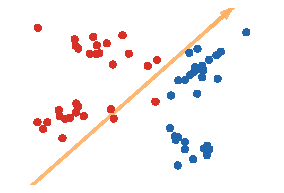
\includegraphics[width=.30\linewidth]{figures/min-sliced-transport-plan/direction.pdf} &
\index{Min-SW}% strictindex
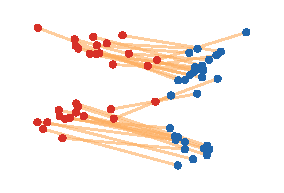
\includegraphics[width=.30\linewidth]{figures/min-sliced-transport-plan/lifted-plan.pdf} &
\index{plan!lifted}% strictindex
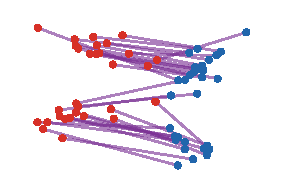
\includegraphics[width=.30\linewidth]{figures/min-sliced-transport-plan/w2-plan.pdf}
\end{tabular}
\caption{\emph{Min-SW lifted plan.} A deterministic angular sweep selects a projection, after which the red and blue atoms are sorted and matched in one dimension. The middle panel lifts this matching back to the plane. Its cost upper-bounds $\Wass_2^2$, but the resulting feasible plan need not equal the quadratic optimal plan shown on the right.}
\label{fig:min-sliced-transport-plan}
\end{figure}

%%%%%%%%%%%%%%%%%%%%%%%%%%%%%%%%%%%%%%%%%%%%%%%%%%%%%%%%%%%%%%%%%%%%%%%%%%%
\section{Quotient Wasserstein and Wasserstein--Procrustes}
\index{quotient!Wasserstein distance}% strictindex
\index{Wasserstein!Procrustes}% strictindex
\label{sec-quotient-wasserstein-procrustes}

This section explains how OT can factor out nuisance symmetries before comparing measures.

\paragraph{Quotient distances.}
\index{quotient!Wasserstein distance}% strictindex
Many comparison problems contain nuisance transformations: two shapes, images or point clouds should be considered close after translating, rotating or otherwise reparametrizing one of them. Quotient Wasserstein distances encode this idea by computing transport after optimizing over a group action. This construction is the metric analogue of passing from objects to shapes modulo symmetries, and connects OT with shape spaces, metamorphosis models and global-invariance variants of transport~\cite{Metamorphosis2005,zemel2017fr,alvarez2018towards}.
\index{group action}% strictindex
\index{shape space}% strictindex

\begin{defn}[Quotient Wasserstein distance]\label{def-quotient-wasserstein}
\index{quotient!Wasserstein distance}% strictindex
	Let a group $\mathcal G$ act on a metric space $(\Xx,d)$ by isometries, and assume that the action preserves finite $p$th moments. Write $g_\sharp\alpha$ for the push-forward of a measure $\alpha$ by $g\in\mathcal G$, and $[\alpha]\eqdef\{g_\sharp\alpha\;:\;g\in\mathcal G\}$ for its orbit. The quotient $p$-Wasserstein distance between the orbits of $\alpha,\beta\in\Pp_p(\Xx)$ is
\index{orbit space}% strictindex
	\[
		\Wass_{p,\mathcal G}([\alpha],[\beta])
		\eqdef
		\inf_{g,h\in\mathcal G}\Wass_p(g_\sharp\alpha,h_\sharp\beta)
		=
		\inf_{g\in\mathcal G}\Wass_p(\alpha,g_\sharp\beta).
	\]
\end{defn}

\begin{prop}[Metric property on the quotient]\label{prop-quotient-wasserstein-metric}
\index{quotient!metric property}% strictindex
	If $\mathcal G$ acts by isometries and preserves $\Pp_p(\Xx)$, then $\Wass_{p,\mathcal G}$ is a pseudo-distance on $\Pp_p(\Xx)$. If the infimum is attained between every pair of orbits, then it is a distance on the orbit space $\Pp_p(\Xx)/\mathcal G$. This applies in particular to continuous actions of compact groups.
\end{prop}

\begin{proof}
	Isometry of the action gives $\Wass_p(g_\sharp\alpha,g_\sharp\beta)=\Wass_p(\alpha,\beta)$, which proves the second formula in Definition~\ref{def-quotient-wasserstein}. Non-negativity and symmetry are inherited from $\Wass_p$. For the triangle inequality, choose $g_1,g_2\in\mathcal G$. Then
	\[
		\Wass_p(\alpha,(g_1)_\sharp\beta)
		+
		\Wass_p(\beta,(g_2)_\sharp\gamma)
		=
		\Wass_p(\alpha,(g_1)_\sharp\beta)
		+
		\Wass_p((g_1)_\sharp\beta,(g_1g_2)_\sharp\gamma).
	\]
	Applying the triangle inequality for $\Wass_p$ and then taking infima over $g_1,g_2$ gives the result. If the infimum is attained and the quotient distance is zero, there exist $g,h\in\mathcal G$ such that $\Wass_p(g_\sharp\alpha,h_\sharp\beta)=0$, hence $g_\sharp\alpha=h_\sharp\beta$ and therefore $[\alpha]=[\beta]$. For a continuous action of a compact group, the objective is continuous on a compact parameter set, so attainment follows. Without attainment, the construction is naturally a metric only after identifying distinct orbits at zero orbit distance.
\end{proof}

\paragraph{Rigid motions and Wasserstein--Procrustes.}
\index{quotient!Wasserstein distance}% strictindex
\index{Euclidean group}% strictindex
\index{Wasserstein!Procrustes}% strictindex
\index{rigid motion}% strictindex
\index{Procrustes!problem}% strictindex

The most common example is the Euclidean group $\mathrm E(d)=\mathrm O(d)\ltimes\RR^d$. Its quotient distance has a standard registration name.
\begin{defn}[Wasserstein--Procrustes distance]\label{def-wasserstein-procrustes}
For $\alpha,\beta\in\Pp_2(\RR^d)$, define
\[
	\operatorname{WP}_2(\alpha,\beta)^2
	\eqdef
	\inf_{\substack{R\in\mathrm O(d),\,t\in\RR^d\\ \pi\in\Couplings(\alpha,\beta)}}
	\int\norm{Rx+t-y}^2\d\pi(x,y).
\]
Restricting \(R\) to \(\mathrm{SO}(d)\) defines the orientation-preserving variant.
\end{defn}
This is the case $p=2$ of the quotient distance; for a general exponent $p$, one replaces the quadratic cost by the $p$th power of the Euclidean distance. Although the translation group is noncompact, the quadratic problem is well behaved: for fixed $R$ and $\pi$, the optimal translation aligns $R\bar x$ with $\bar y$. The remaining rigid step is therefore an orthogonal Procrustes problem over the compact group $\mathrm O(d)$.
\index{Wasserstein!Procrustes}% strictindex
\index{Procrustes!orthogonal}% strictindex
For empirical measures, this couples a transport problem with a rigid registration problem. Classical iterative closest point methods alternate nearest-neighbor assignment and rigid least squares~\cite{BeslMcKay1992ICP}. Wasserstein--Procrustes replaces these hard many-to-one nearest-neighbor correspondences by a mass-preserving OT plan. This makes the registration less tied to sampling density and better suited to ambiguous correspondences.
\index{nearest neighbor}% strictindex
\index{iterative closest point}% strictindex
\index{rigid registration}% strictindex

Two complementary machine-learning formulations clarify the scope of this construction. Grave, Joulin and Berthet~\cite{grave2018unsupervised} formulate unsupervised alignment of high-dimensional embeddings as a Wasserstein--Procrustes problem. In their equal-weight setting, one jointly estimates an orthogonal matrix and a permutation; they use a convex-relaxation initialization and a stochastic large-scale solver, with bilingual lexicon induction as the main application. Alvarez-Melis, Jegelka and Jaakkola~\cite{alvarez2018towards} place the same idea in a broader framework: the coupling and a latent global transformation are optimized jointly over a flexible invariance class because cross-space costs are otherwise ill-defined. The rigid quadratic model and block updates below are the isometric Procrustes specialization of this global-invariance viewpoint.
\index{embedding!alignment}% strictindex
\index{global invariance}% strictindex

This is an extrinsic counterpart of the Gromov--Wasserstein viewpoint developed in Section~\ref{sec-gromov-wasserstein}. Procrustes alignment searches only over ambient rigid motions, whereas GW is invariant under all measure-preserving isometries of metric-measure spaces. The following comparison makes this relation precise.

\begin{prop}[Wasserstein--Procrustes upper certificate]\label{prop-gw-procrustes-upper-certificate}
\index{rigid motion}% strictindex
	Let $p\geq1$ and $\alpha,\beta\in\Pp_p(\RR^d)$. Equip both copies of $\RR^d$ with the Euclidean distance and take $\De(u,v)=|u-v|$ in~\eqref{eq-gw-generic}. Then
	\begin{equation}\label{eq-gw-procrustes-upper}
		\GW((\RR^d,\norm{\cdot},\alpha),(\RR^d,\norm{\cdot},\beta))
		\leq
		2\,\Wass_{p,\mathrm E(d)}([\alpha],[\beta]),
	\end{equation}
	where the quotient distance on the right is defined in Definition~\ref{def-quotient-wasserstein}.
\end{prop}

\begin{proof}
	Fix $g,h\in\mathrm E(d)$. For every $\pi\in\Couplings(\alpha,\beta)$, the push-forward $\widetilde\pi=(g\times h)_\sharp\pi$, where $(g\times h)(x,y)=(g(x),h(y))$, belongs to $\Couplings(g_\sharp\alpha,h_\sharp\beta)$. Since rigid motions preserve Euclidean distances,
	\[
		\norm{g(x)-g(x')}=\norm{x-x'}
		\quad\text{and}\quad
		\norm{h(y)-h(y')}=\norm{y-y'}.
	\]
	The GW objective therefore has the same value at $\pi$ and $\widetilde\pi$. Applying the same argument to $g^{-1}$ and $h^{-1}$ shows that this correspondence is bijective, hence
	\[
		\GW((\RR^d,\norm{\cdot},\alpha),(\RR^d,\norm{\cdot},\beta))
		=
		\GW((\RR^d,\norm{\cdot},g_\sharp\alpha),(\RR^d,\norm{\cdot},h_\sharp\beta)).
	\]
	Proposition~\ref{prop-gw-controlled-by-wasserstein}, applied to the aligned measures on the same Euclidean ground space, now gives
	\[
		\GW((\RR^d,\norm{\cdot},\alpha),(\RR^d,\norm{\cdot},\beta))
		\leq
		2\,\Wass_p(g_\sharp\alpha,h_\sharp\beta).
	\]
	Taking the infimum over $g,h\in\mathrm E(d)$ and using Definition~\ref{def-quotient-wasserstein} proves~\eqref{eq-gw-procrustes-upper}.
\end{proof}

Thus a good Wasserstein--Procrustes registration forces small GW distortion. The converse need not hold: GW may be small because of an intrinsic correspondence that is not induced by an ambient rigid motion. The M\'emoli profile lower bound in Proposition~\ref{prop-memoli-gw-profile-lower-bound} gives the complementary intrinsic lower certificate.
\index{Wasserstein!Procrustes}% strictindex
\index{Gromov-Wasserstein@Gromov--Wasserstein}% strictindex
\index{profile lower bound}% strictindex

The empirical problem naturally suggests an alternating minimization. Given a current rigid motion $(R^{(k)},t^{(k)})$, first compute the OT coupling between the registered source cloud and the target cloud,
\index{rigid motion}% strictindex
\begin{equation}\label{eq-wasserstein-procrustes-coupling-update}
	\P^{(k)}
	\in
	\argmin_{\P\in\CouplingsD(\a,\b)}
	\sum_{i,j}\P_{ij}\norm{R^{(k)}x_i+t^{(k)}-y_j}^2 .
\end{equation}
Then freeze this coupling and update the rigid motion by
\begin{equation}\label{eq-wasserstein-procrustes-rigid-update}
	(R^{(k+1)},t^{(k+1)})
	\in
	\argmin_{R\in\mathrm O(d),\,t\in\RR^d}
	\sum_{i,j}\P^{(k)}_{ij}\norm{Rx_i+t-y_j}^2 ,
\end{equation}
or by the same formula with $R\in\mathrm{SO}(d)$ if orientation should be preserved. The first step is an ordinary discrete OT problem with the current registered cost matrix; the next proposition shows that the second step is an orthogonal Procrustes problem with an explicit singular-value formula.

\begin{prop}[Rigid update for a fixed coupling]\label{prop-wasserstein-procrustes-rigid-update}
\index{Procrustes!rigid update}% strictindex
	Let $\alpha=\sum_i a_i\delta_{x_i}$ and $\beta=\sum_j b_j\delta_{y_j}$, and fix $\P\in\CouplingsD(\a,\b)$. Define
	\[
		\bar x=\sum_i a_i x_i,\qquad
		\bar y=\sum_j b_j y_j,\qquad
		M_\P=\sum_{i,j} \P_{ij}(y_j-\bar y)(x_i-\bar x)^\top .
	\]
	If $M_\P=U\Sigma V^\top$ is a singular value decomposition, then the minimizers over the full orthogonal group of
	\[
		\min_{R\in\mathrm O(d),\,t\in\RR^d}
		\sum_{i,j}\P_{ij}\norm{Rx_i+t-y_j}^2
	\]
	are given by $R^\star=UV^\top$ and $t^\star=\bar y-R^\star\bar x$, up to the usual non-uniqueness when $M_\P$ is rank deficient. If one imposes $R\in\mathrm{SO}(d)$, set
	\[
		D=\diag(1,\ldots,1,\det(UV^\top)),
		\qquad
		R^\star=UDV^\top,
		\qquad
		t^\star=\bar y-R^\star\bar x .
	\]
\end{prop}

\begin{proof}
	For fixed $R$, differentiating with respect to $t$ gives $t=\bar y-R\bar x$. Substituting this value centers the variables and leaves
	\[
		\sum_{i,j}\P_{ij}\norm{R(x_i-\bar x)-(y_j-\bar y)}^2.
	\]
	The two quadratic terms independent of $R$ are fixed, so the problem is equivalent to maximizing
	\[
		\sum_{i,j}\P_{ij}\dotp{R(x_i-\bar x)}{y_j-\bar y}
		=
		\tr(R^\top M_\P).
	\]
	Von Neumann's trace inequality gives $\tr(R^\top U\Sigma V^\top)\leq\tr(\Sigma)$ for $R\in\mathrm O(d)$, with equality for $R=UV^\top$. Under the constraint $R\in\mathrm{SO}(d)$, the same argument applies with the additional determinant constraint on $U^\top R V$, which gives the displayed diagonal correction.
	\end{proof}

\index{Procrustes!alternating minimization}% strictindex
\index{rigid update}% strictindex
	Equations~\eqref{eq-wasserstein-procrustes-coupling-update}--\eqref{eq-wasserstein-procrustes-rigid-update} give a block-coordinate method. The objective is not jointly convex, so the scheme should be read as a registration heuristic for the quotient problem rather than as a global solver. The exact block update moves the rigid motion fully; for visualization or continuation, one may damp the displayed motion between two successive poses.
\index{block-coordinate method}% strictindex

\begin{alg}[Alternating Wasserstein--Procrustes alignment]\label{alg:wasserstein-procrustes}
\index{Wasserstein!Procrustes}% strictindex
\textbf{Input:} Weighted point clouds $(x_i,\a_i)_{i=1}^n$, $(y_j,\b_j)_{j=1}^m$, initial rigid motion $(R^{(0)},t^{(0)})$, tolerance $\mathrm{tol}$, iteration budget $L\geq1$, choice $\mathrm O(d)$ or $\mathrm{SO}(d)$.

\textbf{Output:} Last coupling $\P$ and rigid motion $(R,t)$.

\textbf{Set} $\bar x=\sum_i\a_i x_i$, $\bar y=\sum_j\b_j y_j$, $k=0$ and $\eta_0=+\infty$.

\textbf{While} $\eta_k>\mathrm{tol}$ and $k<L$ \textbf{do}:
\begin{algblock}

\textbf{Set} \(\C_{ij}^{(k)}=\norm{R^{(k)}x_i+t^{(k)}-y_j}^2\).

\textbf{Solve} \(\P^{(k)}\in\argmin_{\P\in\CouplingsD(\a,\b)}\sum_{i,j}\P_{ij}\C_{ij}^{(k)}\).

\textbf{Compute} \(M_{\P^{(k)}}=\sum_{i,j}\P^{(k)}_{ij}(y_j-\bar y)(x_i-\bar x)^\top\).

\textbf{Factorize} \(M_{\P^{(k)}}=U\Sigma V^\top\).

\textbf{Set} \(D=\Id\) for $\mathrm O(d)$; set \(D=\diag(1,\ldots,1,\det(UV^\top))\) for $\mathrm{SO}(d)$.

\textbf{Set} \(R^{(k+1)}=UDV^\top\) and \(t^{(k+1)}=\bar y-R^{(k+1)}\bar x\).

\textbf{Set} \(\eta_{k+1}=\norm{R^{(k+1)}-R^{(k)}}_{\mathrm F}+\norm{t^{(k+1)}-t^{(k)}}\).

\textbf{Set} \(k\leftarrow k+1\).
\end{algblock}
\algreturnskip
\textbf{Solve} \(\P^{(k)}\in\argmin_{\P\in\CouplingsD(\a,\b)}\sum_{i,j}\P_{ij}\norm{R^{(k)}x_i+t^{(k)}-y_j}^2\).

\textbf{Return} \(\P^{(k)},R^{(k)},t^{(k)}\).
\end{alg}

Figure~\ref{fig:wasserstein-procrustes-rigid-motion} follows this block-coordinate scheme through a deliberately large translation, showing how the transport correspondences and the rigid registration stabilize together.

\begin{figure}[H]
\centering
\setlength{\tabcolsep}{2pt}
\begin{tabular}{@{}ccccc@{}}
\small iter. 1 & \small iter. 2 & \small iter. 3 & \small iter. 5 & \small iter. 10 \\[-.15em]
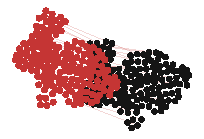
\includegraphics[width=.19\linewidth]{figures/wasserstein-procrustes-rigid-motion/iter-01.pdf} &
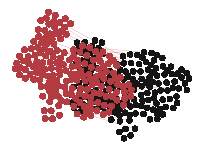
\includegraphics[width=.19\linewidth]{figures/wasserstein-procrustes-rigid-motion/iter-02.pdf} &
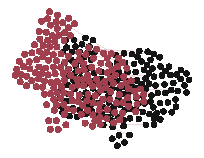
\includegraphics[width=.19\linewidth]{figures/wasserstein-procrustes-rigid-motion/iter-03.pdf} &
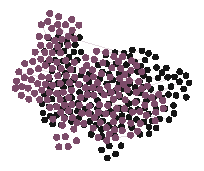
\includegraphics[width=.19\linewidth]{figures/wasserstein-procrustes-rigid-motion/iter-05.pdf} &
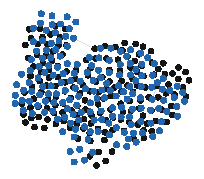
\includegraphics[width=.19\linewidth]{figures/wasserstein-procrustes-rigid-motion/iter-10.pdf}
\end{tabular}
\caption{\emph{Wasserstein--Procrustes alignment of two bunny silhouettes under a strong translation and a moderate rotation.} The target silhouette is shown in black. The moving source silhouette is sampled by farthest-point sampling and colored from red to blue at iterations \(1,2,3,5,10\). Each step solves an equal-weight OT assignment, then updates the rigid motion by the closed-form Procrustes formula of Proposition~\ref{prop-wasserstein-procrustes-rigid-update}; faint segments show selected correspondences of the current OT assignment. The displayed motion is damped only to make the registration path visible, while the underlying update is the block-coordinate method of Algorithm~\ref{alg:wasserstein-procrustes}.}
\label{fig:wasserstein-procrustes-rigid-motion}
\end{figure}

%%%%%%%%%%%%%%%%%%%%%%%%%%%%%%%%%%%%%%%%%%%%%%%%%%%%%%%%%%%%%%%%%%%%%%%%%%%
\section{Vector Quantiles and Linear Optimal Transport}
\index{vector quantile}% strictindex
\index{linear!OT}% strictindex
\label{sec-linear-ot}
\label{sec-vector-quantiles-linearized-transport}

Linear OT starts from the multivariate analogue of quantile coordinates. The one-dimensional quantile function represents a probability measure by the monotone map sending a fixed reference law to it; in dimension $d>1$, Brenier's theorem gives the corresponding construction after choosing an absolutely continuous reference probability $\alpha_{\rm ref}$, typically the uniform law on a convex body or a standard Gaussian.
\index{probability measure}% strictindex
\index{Brenier!theorem}% strictindex
\index{quantile!function}% strictindex
\index{linear!OT}% strictindex

\paragraph{Vector quantiles.}
\index{vector quantile}% strictindex

Assume that $\alpha_{\rm ref}$ is absolutely continuous. For a target law $\al$ with finite second moment, its vector quantile relative to $\alpha_{\rm ref}$ is the Brenier map
\index{Brenier!map}% strictindex
\[
	\T_\al=\nabla\phi_\al,
	\qquad
	(\T_\al)_\sharp\alpha_{\rm ref}=\al,
\]
or equivalently the solution of
\[
	\min_{\T_\sharp\alpha_{\rm ref}=\al}
	\int \norm{x-\T(x)}^2\d\alpha_{\rm ref}(x).
\]
This construction is canonical only after fixing $\alpha_{\rm ref}$: changing the reference law changes the coordinates used to represent $\al$. The same transport-based quantile map has been used in several complementary statistical directions. Conditional vector quantile regression replaces scalar conditional quantiles by conditional Brenier maps~\cite{carlier2016vectorquantile,carlier2016vector}; Monge--Kantorovich ranks and depth use transports to a spherical reference~\cite{chernozhukov2017monge}; center-outward distribution and quantile functions build multivariate ranks and signs from the forward and inverse maps~\cite{hallin2021distribution}; and scalable nonlinear vector quantile regression learns such conditional maps with flexible models~\cite{rosenberg2023fast}.
\index{quantile!function}% strictindex
\index{conditional!quantile}% strictindex
\index{vector quantile}% strictindex
\index{Brenier!map}% strictindex

\paragraph{Linearized Wasserstein coordinates.}
\index{Wasserstein!coordinate}% strictindex

Linear OT replaces a nonlinear transport distance by a Hilbert norm between reference maps. It is useful when one reference measure is fixed and many nearby distributions must be compared cheaply. Let $T_\alpha$ be the Brenier map pushing $\alpha_{\rm ref}$ to $\alpha$, understood as an element of $L^2(\alpha_{\rm ref};\RR^d)$ and hence defined only $\alpha_{\rm ref}$-almost everywhere. The linear OT embedding is
\index{reference!measure}% strictindex
\index{linear!OT}% strictindex
\begin{defn}[Linear optimal-transport embedding]\label{def-lot-embedding}
Fix an absolutely continuous reference measure $\alpha_{\rm ref}\in\Pp_2(\RR^d)$, and let $T_\alpha$ denote the Brenier map from $\alpha_{\rm ref}$ to $\alpha\in\Pp_2(\RR^d)$. Then
\begin{equation}\label{eq-lot-embedding}
	\alpha \mapsto T_\alpha-\Id\in L^2(\alpha_{\rm ref};\RR^d),
	\qquad
	\LOT_{\alpha_{\rm ref}}(\alpha,\beta)=\norm{T_\alpha-T_\beta}_{L^2(\alpha_{\rm ref})}.
\end{equation}
\end{defn}
If one of the two targets equals the reference, the linearized distance is exact. For instance,
\[
	\LOT_{\alpha_{\rm ref}}(\alpha_{\rm ref},\alpha)
	=
	\norm{T_\alpha-\Id}_{L^2(\alpha_{\rm ref})}
	=
	\Wass_2(\alpha_{\rm ref},\alpha).
\]
For two arbitrary targets, the coupling $(T_\alpha,T_\beta)_\sharp\alpha_{\rm ref}$ is admissible but not generally optimal, so $\LOT_{\alpha_{\rm ref}}$ is a tangent-space approximation of the Wasserstein geometry. Introduced for the analysis of image populations~\cite{wang2013linear}, LOT has subsequently been used for continuous image-pattern analysis~\cite{kolouri2016continuous}, provable classification of transformed distributions~\cite{moosmuller2023linear}, collider-event analysis~\cite{cai2020linearized}, and scalable Wasserstein dimensionality reduction~\cite{cloninger2025linearized}. Uniqueness of the Brenier maps shows that $\LOT_{\alpha_{\rm ref}}$ is itself a distance on the target measures for which these maps are defined.
For a family $(\alpha_s)_s$ with weights $(\lambda_s)_s$, the linearized barycenter is obtained by averaging maps,
\[
	\bar T=\sum_s\lambda_s T_{\alpha_s},
	\qquad
	\bar\alpha_{\LOT}=\bar T_\sharp\alpha_{\rm ref}.
\]
This is exact in one dimension, where quantile functions linearize $\Wass_2$, and it is especially useful when many barycenters with changing weights must be evaluated quickly.
\index{quantile!function}% strictindex

Figure~\ref{fig:dualnorms-linear-ot-embedding} makes the LOT embedding explicit: map averaging is exact in one-dimensional quantile coordinates, whereas in two dimensions its linearized barycenter can differ from the genuine McCann midpoint.

\begin{figure}[htbp]
\centering
\setlength{\tabcolsep}{2pt}
\begin{tabular}{@{}ccc@{}}
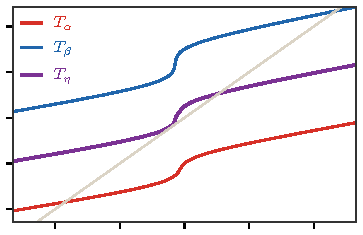
\includegraphics[width=.45\linewidth]{figures/dualnorms-linear-ot-embedding/displacements-1d.pdf} &
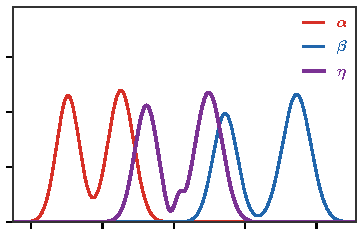
\includegraphics[width=.45\linewidth]{figures/dualnorms-linear-ot-embedding/barycenter-1d.pdf} \\[-.1em]
\small 1D maps $T_\alpha,T_\beta,T_\gamma$ & \small measures $\alpha,\beta,\gamma$
\end{tabular}

\vspace{.25em}
\begin{tabular}{@{}ccc@{}}
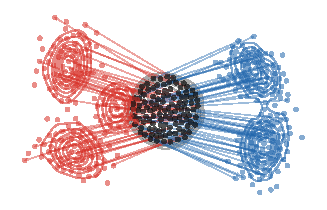
\includegraphics[width=.30\linewidth]{figures/dualnorms-linear-ot-embedding/targets-2d.pdf} &
\index{linear!OT}% strictindex
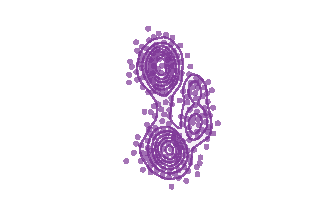
\includegraphics[width=.30\linewidth]{figures/dualnorms-linear-ot-embedding/barycenter-2d.pdf} &
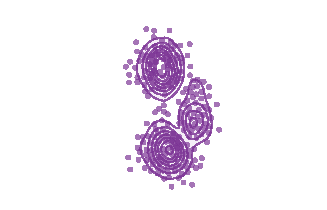
\includegraphics[width=.30\linewidth]{figures/dualnorms-linear-ot-embedding/barycenter-2d-ot.pdf} \\[-.1em]
\small maps from $\alpha_{\rm ref}$ to $\alpha,\beta$ &
\small linearized barycenter $\bar T_\sharp\alpha_{\rm ref}$ &
\small McCann midpoint
\end{tabular}
\caption{\emph{Linear OT coordinates.} Fixing a reference measure $\alpha_{\rm ref}$ turns each target into a map $T_\alpha$ from $\alpha_{\rm ref}$ to $\alpha$, or equivalently into the displacement field $T_\alpha-\Id$. In one dimension this is exactly the quantile parametrization of $\Wass_2$, so averaging the maps toward a two-component $\alpha$ and a two-component $\beta$ gives the true Wasserstein barycenter. In two dimensions, the first panel shows the reference-to-target maps, computed on dense clouds and displayed on farthest-point subsets, with $\beta$ represented by two Gaussian components. The middle purple panel shows the linearized barycenter obtained by averaging the two maps from $\alpha_{\rm ref}$. The right purple panel shows the genuine McCann midpoint between $\alpha$ and $\beta$, obtained by solving a direct OT problem between the two target clouds and interpolating at $t=1/2$.}
\index{Wasserstein!barycenter}% strictindex
\index{reference!measure}% strictindex
\index{linear!OT}% strictindex
\label{fig:dualnorms-linear-ot-embedding}
\end{figure}

The usefulness of these coordinates depends on controlling how much they distort the underlying Wasserstein geometry. The following global estimate is therefore important: LOT always dominates $\Wass_2$, while on compact supports with a uniform reference it remains H\"older-continuous with respect to perturbations measured by $\Wass_1$.

\begin{prop}[Quantitative stability of linear OT]\label{prop-linear-ot-stability}
	Let $X,Y\subset\RR^d$ be compact convex sets, assume that $X$ has positive Lebesgue measure, and let $\alpha_{\rm ref}$ be normalized Lebesgue measure on $X$. Then there exists a constant $C=C(d,X,Y)$ such that, for all $\alpha,\beta\in\Pp(Y)$,
\index{Brenier!map}% strictindex
	\[
		\Wass_2(\alpha,\beta)\leq \LOT_{\alpha_{\rm ref}}(\alpha,\beta)
		\quad\text{and}\quad
		\LOT_{\alpha_{\rm ref}}(\alpha,\beta)
		\leq
		C\Wass_1(\alpha,\beta)^{2/15}.
	\]
\end{prop}
\begin{proof}
	The first inequality is immediate: $(T_\alpha,T_\beta)_\sharp\alpha_{\rm ref}$ is a feasible coupling between $\alpha$ and $\beta$. The second inequality is the quantitative stability theorem of M\'erigot, Delalande and Chazal~\cite{merigot2020stability}. Its proof first controls the difference of the two Kantorovich potentials in terms of $\Wass_1(\alpha,\beta)$, then combines convexity and interpolation estimates to control the gradients in $L^2(\alpha_{\rm ref})$; the resulting dimension-independent H\"older exponent is $2/15$.
\index{feasible coupling}% strictindex
\index{Monge-Ampere@Monge--Amp\`ere!equation}% strictindex
\index{quantile!function}% strictindex
	In one dimension, quantile functions make the embedding isometric and the exponent improves to one. In several dimensions, the theorem is global but only H\"older; it should not be read as a global Lipschitz estimate in $\Wass_2$.
\end{proof}

\begin{rem}[Three Hilbertian embeddings of measures]\label{rem-three-hilbertian-measure-embeddings}
\index{Hilbertian!embedding}% strictindex
	Several constructions in this text embed measures into Hilbert spaces, but they encode different geometries. Kernel mean embeddings send $\alpha$ to $\int k(x,\cdot)\d\alpha(x)$ in an RKHS and lead to MMD distances; see Section~\ref{sec-rkhs-mmd}. Quadratic sliced Wasserstein sends a measure to the collection of one-dimensional quantile functions of its projections, viewed in $L^2(\Sphere^{d-1}\times[0,1])$; see Section~\ref{sec-sliced-wasserstein}. Linear OT sends $\alpha$ to the displacement field $T_\alpha-\Id$ from a fixed reference $\alpha_{\rm ref}$ in $L^2(\alpha_{\rm ref};\RR^d)$. The first construction is linear in the measure and depends on the kernel, the second is nonlinear but reduces OT to projected one-dimensional quantiles, and the third is a tangent approximation to the full Wasserstein geometry around a chosen reference.
\index{sliced Wasserstein!distance}% strictindex
\index{RKHS}% strictindex
\index{maximum mean discrepancy}% strictindex
\index{kernel!mean embedding}% strictindex
\index{linear!OT}% strictindex
\end{rem}

\paragraph{Principal components in linear OT coordinates.}
\index{principal component analysis}% strictindex
\index{linear!OT}% strictindex

The preceding embedding turns probability measures into displacement fields in a fixed Hilbert chart, so ordinary principal component analysis can be applied to deformations rather than to densities. Given training measures \((\alpha_i)_{i=1}^N\), set
\[
	z_i \eqdef T_{\alpha_i}-\Id,
	\qquad
	\bar z \eqdef \frac1N\sum_{i=1}^N z_i .
\]
The map \(\Id+\bar z\) defines the linear OT mean \((\Id+\bar z)_\sharp\alpha_{\rm ref}\). The empirical covariance operator on \(L^2(\alpha_{\rm ref};\RR^d)\) is the finite-rank operator
\[
	\mathcal C_{\LOT} h
	\eqdef
	\frac1N\sum_{i=1}^N
	\dotp{z_i-\bar z}{h}_{L^2(\alpha_{\rm ref})}
	(z_i-\bar z),
\]
and its leading orthonormal eigenvectors \(e_k\) define the principal linear OT modes. Equivalently, one diagonalizes the \(N\times N\) Gram matrix \(G_{ij}=\frac1N\dotp{z_i-\bar z}{z_j-\bar z}_{L^2(\alpha_{\rm ref})}\). If \(Gv^{(k)}=\lambda_k v^{(k)}\) with \(\lambda_k>0\) and \(\norm{v^{(k)}}=1\), then
\[
	e_k=\frac{1}{\sqrt{N\lambda_k}}\sum_{i=1}^N v_i^{(k)}(z_i-\bar z)
\]
is the corresponding unit eigenvector of \(\mathcal C_{\LOT}\). The score of \(\alpha_i\) along mode \(e_k\) is
\[
	a_{i,k} \eqdef \dotp{z_i-\bar z}{e_k}_{L^2(\alpha_{\rm ref})} .
\]
A low-rank reconstruction, or a synthetic excursion with prescribed coefficients \(a=(a_1,\ldots,a_m)\), is then obtained by pushing the reference through
\[
	T_a(x) \eqdef x+\bar z(x)+\sum_{k=1}^m a_k e_k(x),
	\qquad
	\alpha_a \eqdef (T_a)_\sharp\alpha_{\rm ref} .
\]
For small excursions around the mean displacement, this gives a practical tangent-space PCA for probability measures: it captures dominant modes of deformation while avoiding repeated pairwise OT computations. For large coefficients, \(T_a\) may fail to be the Brenier map from \(\alpha_{\rm ref}\) to \(\alpha_a\), and may even leave the regular chart where \(T_a\) is a gradient of a convex function. Thus \(a\mapsto \alpha_a\) should be read as a chart-dependent linearized visualization rather than as an intrinsic Wasserstein geodesic. This LOT-PCA viewpoint was introduced for image variability analysis in~\cite{wang2013linear} and developed in transport-based signal analysis~\cite{thorpe2017transportation,kolouri2017optimal}; it complements intrinsic principal-geodesic or geodesic-PCA approaches, which optimize directly in the curved Wasserstein space~\cite{SeguyCuturi,bigot2017geodesic}.
\index{covariance!operator}% strictindex
\index{principal component analysis}% strictindex
\index{Brenier!map}% strictindex
\index{Wasserstein!geodesic}% strictindex

Figure~\ref{fig:linear-ot-1d-pca} first shows the exact one-dimensional case. A large training set of well-separated two-Gaussian mixtures is generated with moderate component-wise location and scale variations, although only representative densities are displayed. Each density is embedded by its quantile function on a fine grid, ordinary PCA is performed in \(L^2(0,1)\), and the displayed modes are obtained by converting quantile excursions back into densities.
\index{quantile!function}% strictindex

\begin{figure}[htbp]
\centering
\setlength{\tabcolsep}{3pt}
\begin{tabular}{@{}cc@{}}
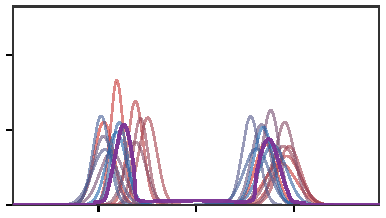
\includegraphics[width=.47\linewidth]{figures/linear-ot-1d-pca/dataset.pdf} &
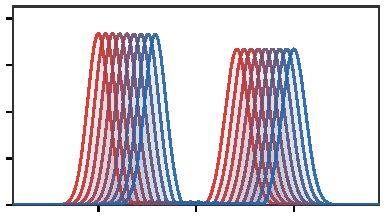
\includegraphics[width=.47\linewidth]{figures/linear-ot-1d-pca/mode-1.pdf}
\\[-.1em]
\small training densities and quantile mean & \small first quantile-PCA mode
\\[.35em]
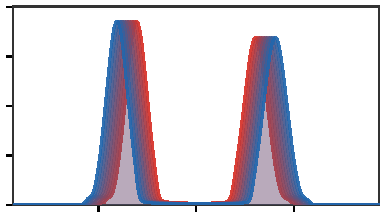
\includegraphics[width=.47\linewidth]{figures/linear-ot-1d-pca/mode-2.pdf} &
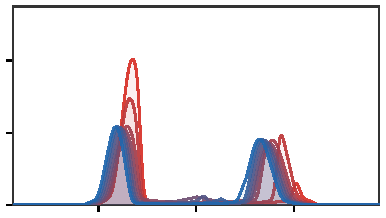
\includegraphics[width=.47\linewidth]{figures/linear-ot-1d-pca/mode-3.pdf}
\\[-.1em]
\small second quantile-PCA mode & \small third quantile-PCA mode
\end{tabular}
\caption{\emph{One-dimensional linear OT PCA for synthetic two-Gaussian mixtures.} The PCA is fit on a large training ensemble, while the dataset panel displays only representative densities and the quantile average in violet. Each mode panel shows densities obtained from \(Q_{\bar\alpha}+a e_k\), using slightly extrapolated coefficients \(a\) increasing from red to blue. Since the embedding is the exact quantile parametrization \(Q_\alpha\in L^2(0,1)\), this PCA is performed in exact Wasserstein coordinates rather than in an approximate tangent chart.}
\index{linear!OT}% strictindex
\index{quantile!function}% strictindex
\index{principal component analysis}% strictindex
\label{fig:linear-ot-1d-pca}
\end{figure}

Figure~\ref{fig:linear-ot-mnist-pca} then illustrates a regularized numerical approximation of the same construction on MNIST digit-zero images. Each image is normalized as a probability measure on the pixel grid. A Sinkhorn barycenter is used as the reference \(\alpha_{\rm ref}\), entropic couplings from \(\alpha_{\rm ref}\) to the training images are converted into barycentric-projection maps, and PCA is applied to the resulting approximate displacement fields.
\index{Sinkhorn!barycenter}% strictindex
\index{barycentric!projection}% strictindex

\begin{figure}[htbp]
\centering
\setlength{\tabcolsep}{2pt}
\begin{tabular}{@{}c@{\hspace{4pt}}c@{}}
\begin{tabular}[c]{@{}c@{}}
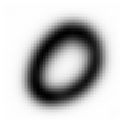
\includegraphics[width=.16\linewidth]{figures/linear-ot-mnist-pca/barycenter.pdf}
\\[-.1em]
\small Sinkhorn barycenter
\end{tabular}
&
\begin{tabular}[c]{@{}cc@{}}

\includegraphics[width=.39\linewidth]{figures/linear-ot-mnist-pca/mode-1.pdf} &

\includegraphics[width=.39\linewidth]{figures/linear-ot-mnist-pca/mode-2.pdf}
\\[-.1em]
\small first LOT-PCA mode & \small second LOT-PCA mode
\\[.35em]

\includegraphics[width=.39\linewidth]{figures/linear-ot-mnist-pca/mode-3.pdf} &
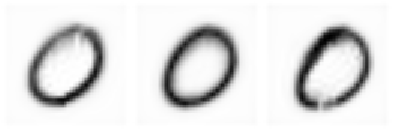
\includegraphics[width=.39\linewidth]{figures/linear-ot-mnist-pca/mode-4.pdf}
\\[-.1em]
\small third LOT-PCA mode & \small fourth LOT-PCA mode
\end{tabular}
\end{tabular}
\caption{\emph{Principal components in linear OT coordinates for MNIST digit-zero histograms.} The left panel shows the Sinkhorn barycenter reference \(\alpha_{\rm ref}\). Each mode panel is a triptych obtained by pushing \(\alpha_{\rm ref}\) through \(x\mapsto x+\bar z(x)+a e_k(x)\) with a negative, zero, and positive coefficient \(a\). The displayed densities use white for zero displayed mass and black for high displayed mass; the underlying transport computations still use the original densities, where high pixel values carry the mass. The modes capture rotations, aspect-ratio changes, and stroke-thickness deformations in the tangent chart around the barycenter.}
\index{linear!OT}% strictindex
\index{principal component analysis}% strictindex
\label{fig:linear-ot-mnist-pca}
\end{figure}


%%%%%%%%%%%%%%%%%%%%%%%%%%%%%%%%%%%%%%%%%%%%%%%%%%%%%%%%%%%%%%%%%%%%%%%%%%%
\section{Spectral and Robust Wasserstein Distances}
\index{Wasserstein!distance}% strictindex
\index{spectral Wasserstein!distance}% strictindex
\index{robust!Wasserstein}% strictindex
\index{robust!Wasserstein distance}% strictindex
\label{sec-spectral-subspace-wasserstein}

Spectral OT changes the scalar quadratic cost by measuring the whole displacement covariance through a matrix gauge. The same object admits a robust projected formulation: instead of fixing one projection, one maximizes over the polar set of the gauge. Subspace robust OT is the important non-convex rank-constrained version of this idea~\cite{paty2019subspace}; spectral gauges provide its convex minimax counterpart and connect to recent spectral-gradient viewpoints such as Muon dynamics~\cite{peyre2026muon}.
\index{spectral!gauge}% strictindex
\index{rank constraint}% strictindex
\index{minimax}% strictindex
\index{polar set}% strictindex
\index{projected formulation}% strictindex
\index{Muon algorithm}% strictindex
\index{displacement covariance}% strictindex
\index{quadratic!cost}% strictindex

\begin{defn}[Monotone spectral gauge]\label{def-monotone-spectral-gauge}
\index{spectral!gauge}% strictindex
\index{monotone!spectral gauge}% strictindex
	A monotone spectral gauge on positive semidefinite matrices is a convex, positively $1$-homogeneous map $\gamma:\mathbb S_+^d\to\RR_+$ such that $\gamma(M)=0$ only for $M=0$, $\gamma(QM\transp{Q})=\gamma(M)$ for every orthogonal matrix $Q$, and
\index{positive!semidefinite matrix}% strictindex
	\[
		0\preceq M\preceq N
		\quad\Longrightarrow\quad
		\gamma(M)\leq\gamma(N).
	\]
	For $1\leq q\leq+\infty$, the Schatten gauge
\index{Schatten norm}% strictindex
	\[
		\gamma_q(M)\eqdef\norm{M}_{S_q}
		=
		\begin{cases}
			\pa{\sum_{i=1}^d\lambda_i(M)^q}^{1/q}, & 1\leq q<+\infty,\\
			\lambda_{\max}(M), & q=+\infty,
		\end{cases}
	\]
	is a monotone spectral gauge. The cases $q=1$, $q=2$ and $q=+\infty$ are respectively the trace, Frobenius and spectral gauges.
\index{trace!gauge}% strictindex
\index{Frobenius norm}% strictindex
\index{spectral!gauge}% strictindex
\end{defn}
The monotonicity condition means that increasing the displacement covariance in Loewner order cannot decrease the transport penalty.
\index{displacement covariance}% strictindex

\begin{defn}[Spectral Wasserstein distance]\label{def-spectral-wasserstein}
\index{Wasserstein!distance}% strictindex
\index{spectral Wasserstein!distance}% strictindex
	Let $\gamma$ be a monotone spectral gauge. For a coupling $\pi\in\Couplings(\alpha,\beta)$, define its displacement covariance
\index{spectral!gauge}% strictindex
	\[
		M_\pi\eqdef\int (x-y)(x-y)^\top\d\pi(x,y).
	\]
	The spectral Wasserstein distance associated with $\gamma$ is
	\eql{\label{eq-spectral-wasserstein}
		\Wass_\gamma(\alpha,\beta)^2
		\eqdef
		\inf_{\pi\in\Couplings(\alpha,\beta)}\gamma(M_\pi).
	}
\end{defn}

The special case $\gamma(M)=\tr(M)$ gives the usual quadratic Wasserstein distance $\Wass_2$. The spectral gauge $\gamma(M)=\lambda_{\max}(M)$ instead measures the worst transported variance direction. For $A\succeq0$, define the quadratic projected transport cost
\index{Wasserstein!distance}% strictindex
\index{spectral!gauge}% strictindex
\eql{\label{eq-quadratic-projected-cost}
	\Wass_{2,A}(\alpha,\beta)^2
	\eqdef
	\inf_{\pi\in\Couplings(\alpha,\beta)}
	\int (x-y)^\top A(x-y)\d\pi(x,y)
	=
	\Wass_2((A^{1/2})_\sharp\alpha,(A^{1/2})_\sharp\beta)^2.
}
The last equality remains valid when $A$ is singular. One inequality follows by projecting any coupling of $(\alpha,\beta)$; for the converse, disintegrate $\alpha$ and $\beta$ over their $A^{1/2}$-images and lift a coupling of the projected measures by conditionally coupling the fibers.
The polar set of the gauge is
\index{polar set}% strictindex
\eql{\label{eq-spectral-polar-set}
	\mathcal B_\gamma
	\eqdef
	\enscond{A\succeq0}{\tr(AM)\leq\gamma(M)\quad\text{for all }M\succeq0},
}
so that, for a closed gauge, $\gamma(M)=\sup_{A\in\mathcal B_\gamma}\tr(AM)$. For the Schatten gauge $\gamma_q$, Schatten H\"older duality gives
\index{Schatten norm}% strictindex
\index{Holder inequality@H\"older inequality}% strictindex
\[
	\mathcal B_{\gamma_q}
	=
	\enscond{A\succeq0}{\norm{A}_{S_{q^\ast}}\leq1},
	\qquad
	\frac1q+\frac1{q^\ast}=1,
\]
with the usual endpoint conventions. Thus the trace gauge has polar set $\{A:0\preceq A\preceq\Id\}$, the Frobenius gauge is self-polar on $\mathbb S_+^d$, and the spectral gauge has polar set $\{A\succeq0:\tr(A)\leq1\}$.

\begin{prop}[Robust representation and metric equivalence]\label{prop-spectral-wasserstein-robust}
\index{robust!representation}% strictindex
\index{metric!equivalence}% strictindex
	Assume, for simplicity, that the measures are compactly supported and that $\gamma$ is closed and finite on the positive semidefinite cone. Then
	\[
		\Wass_\gamma(\alpha,\beta)^2
		=
		\sup_{A\in\mathcal B_\gamma}
		\Wass_{2,A}(\alpha,\beta)^2.
	\]
	If there exist constants $0<a\leq b<+\infty$ such that $a\Id\in\mathcal B_\gamma$ and $\mathcal B_\gamma\subset\enscond{A}{0\preceq A\preceq b\Id}$, equivalently
	\[
		a\tr(M)\leq\gamma(M)\leq b\tr(M)
		\qquad (M\succeq0),
	\]
	then
	\[
		\sqrt a\,\Wass_2(\alpha,\beta)
		\leq
		\Wass_\gamma(\alpha,\beta)
		\leq
		\sqrt b\,\Wass_2(\alpha,\beta).
	\]
	The robust representation proves that $\Wass_\gamma$ is a distance: the supremum of pseudodistances gives symmetry and the triangle inequality, while the lower comparison with $\Wass_2$ gives definiteness. When $\gamma$ is the restriction of a norm to the positive semidefinite cone, these bounds hold automatically in finite dimension, so $\Wass_\gamma$ is equivalent to $\Wass_2$ on measures with finite second moments.
\end{prop}

\begin{proof}
	Using the polar representation of $\gamma$,
	\[
		\Wass_\gamma(\alpha,\beta)^2
		=
		\inf_{\pi\in\Couplings(\alpha,\beta)}
		\sup_{A\in\mathcal B_\gamma}\tr(AM_\pi).
	\]
	The coupling set is convex and compact for weak convergence under compact support. Since $\gamma$ is a finite gauge on a finite-dimensional cone and vanishes only at the origin, it is equivalent to the trace norm on the slice $\tr(M)=1$, so $\mathcal B_\gamma$ is convex and compact. The map $(\pi,A)\mapsto\tr(AM_\pi)$ is affine in each variable and continuous. Sion's minimax theorem gives
\index{minimax}% strictindex
\index{trace!norm}% strictindex
\index{weak!convergence}% strictindex
	\[
		\inf_\pi\sup_{A\in\mathcal B_\gamma}\tr(AM_\pi)
		=
		\sup_{A\in\mathcal B_\gamma}\inf_\pi\tr(AM_\pi)
		=
		\sup_{A\in\mathcal B_\gamma}\Wass_{2,A}(\alpha,\beta)^2.
	\]
	For fixed $A\succeq0$, $\Wass_{2,A}$ is the Wasserstein pseudodistance associated with the seminorm $x\mapsto\norm{A^{1/2}x}$. Since all terms are nonnegative, the robust identity also gives
	\[
		\Wass_\gamma(\alpha,\beta)
		=
		\sup_{A\in\mathcal B_\gamma}\Wass_{2,A}(\alpha,\beta).
	\]
	A supremum of pseudodistances is symmetric and satisfies the triangle inequality.
\index{triangle inequality}% strictindex

	If $a\Id\in\mathcal B_\gamma$ and $A\preceq b\Id$ for all $A\in\mathcal B_\gamma$, then
	\[
		a\Wass_2(\alpha,\beta)^2
		=
		\Wass_{2,a\Id}(\alpha,\beta)^2
		\leq
		\Wass_\gamma(\alpha,\beta)^2
		\leq
		b\Wass_2(\alpha,\beta)^2,
	\]
	which proves definiteness and equivalence with $\Wass_2$. The equivalence between these operator bounds and $a\tr(M)\leq\gamma(M)\leq b\tr(M)$ follows directly from the polar formula. In finite dimension, any norm restricted to the positive semidefinite cone is equivalent to the trace norm on that cone. The finite-second-moment case follows by truncation when these norm-equivalence bounds hold.
\index{polar formula}% strictindex
\index{operator bound}% strictindex
\index{trace!norm}% strictindex
\end{proof}

\begin{defn}[Subspace robust Wasserstein]\label{def-subspace-robust-wasserstein}
\index{robust!Wasserstein}% strictindex
\index{subspace!robust Wasserstein}% strictindex
	For $1\leq k\leq d$, the Paty--Cuturi subspace robust Wasserstein distance is
\index{Wasserstein!distance}% strictindex
\index{robust!Wasserstein distance}% strictindex
	\[
		\SRW_{2,k}(\alpha,\beta)
		\eqdef
		\sup_{\transp{U}U=\Id_k}
		\Wass_2((\transp{U})_\sharp\alpha,(\transp{U})_\sharp\beta)
		=
		\sup_{P^2=P=\transp{P},\ \tr(P)=k}\Wass_{2,P}(\alpha,\beta).
	\]
\end{defn}

For the Ky Fan gauge
\[
	\gamma_k(M)=\sum_{\ell=1}^k\lambda_\ell(M),
\]
where the eigenvalues are sorted in decreasing order, the polar set is
\index{polar set}% strictindex
\[
	\mathcal B_{\gamma_k}=\enscond{A}{0\preceq A\preceq\Id,\ \tr(A)\leq k}.
\]
Thus $k=d$ gives $\gamma_d(M)=\tr(M)$ and recovers $\Wass_2$. The convex hull of rank-$k$ projectors is
\[
	\enscond{A}{0\preceq A\preceq\Id,\ \tr(A)=k},
\]
and, since $M\succeq0$, the associated support function is the same Ky Fan gauge. Thus $\Wass_{\gamma_k}$ is the convexified spectral counterpart of $\SRW_{2,k}$, while $\SRW_{2,k}$ keeps the original non-convex rank constraint. More precisely,
\[
	\SRW_{2,k}(\alpha,\beta)
	\leq
	\Wass_{\gamma_k}(\alpha,\beta)
	\leq
	\Wass_2(\alpha,\beta),
	\qquad
	\sqrt{\frac{k}{d}}\,\Wass_2(\alpha,\beta)
	\leq
	\Wass_{\gamma_k}(\alpha,\beta),
	\]
	because
	\[
		\left\{\frac{k}{d}\Id\right\}
		\cup
		\enscond{P}{P^2=P=P^\top,\ \tr(P)=k}
		\subset \mathcal B_{\gamma_k}
		\subset
		\enscond{A}{0\preceq A\preceq\Id}.
	\]
	For $k=1$, $\gamma_1(M)=\lambda_{\max}(M)$ and $\mathcal B_{\gamma_1}=\enscond{A\succeq0}{\tr(A)\leq1}$.
This top-eigenvalue spectral Wasserstein geometry is the case connected to Muon-type spectral dynamics in~\cite{peyre2026muon}.
\index{spectral!dynamics}% strictindex
\index{Muon algorithm}% strictindex
\index{spectral Wasserstein!distance}% strictindex

Figure~\ref{fig:spectral-wasserstein-gauge} compares the trace and top-eigenvalue geometries at both levels: the selected transport plans and the displacement interpolations they induce.

\begin{figure}[H]
\centering
\setlength{\tabcolsep}{3pt}
\begin{tabular}{@{}cc@{}}
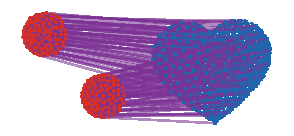
\includegraphics[width=.34\linewidth]{figures/spectral-wasserstein-gauge/trace-coupling.pdf} &
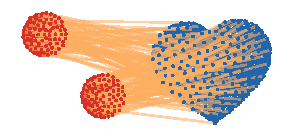
\includegraphics[width=.34\linewidth]{figures/spectral-wasserstein-gauge/lambda-max-coupling.pdf}
\\[-.1em]
\small trace-gauge coupling & \small $\lambda_{\max}$-gauge coupling
\index{trace!gauge}% strictindex
\end{tabular}
\\[.35em]
\begin{tabular}{@{}ccccc@{}}
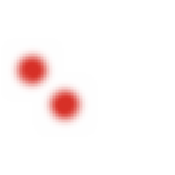
\includegraphics[width=.17\linewidth]{figures/spectral-wasserstein-gauge/trace-density-t000.pdf} &
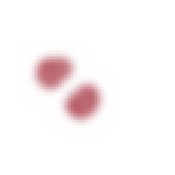
\includegraphics[width=.17\linewidth]{figures/spectral-wasserstein-gauge/trace-density-t025.pdf} &
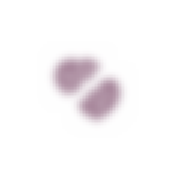
\includegraphics[width=.17\linewidth]{figures/spectral-wasserstein-gauge/trace-density-t050.pdf} &
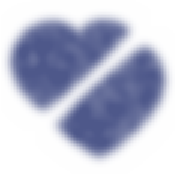
\includegraphics[width=.17\linewidth]{figures/spectral-wasserstein-gauge/trace-density-t075.pdf} &

\includegraphics[width=.17\linewidth]{figures/spectral-wasserstein-gauge/trace-density-t100.pdf} \\[-.1em]
\multicolumn{5}{c}{\small trace-gauge interpolation} \\[.2em]
\index{trace!gauge}% strictindex
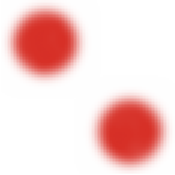
\includegraphics[width=.17\linewidth]{figures/spectral-wasserstein-gauge/lambda-max-density-t000.pdf} &
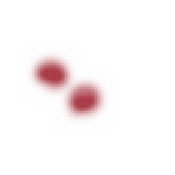
\includegraphics[width=.17\linewidth]{figures/spectral-wasserstein-gauge/lambda-max-density-t025.pdf} &
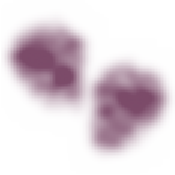
\includegraphics[width=.17\linewidth]{figures/spectral-wasserstein-gauge/lambda-max-density-t050.pdf} &
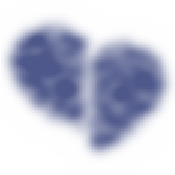
\includegraphics[width=.17\linewidth]{figures/spectral-wasserstein-gauge/lambda-max-density-t075.pdf} &

\includegraphics[width=.17\linewidth]{figures/spectral-wasserstein-gauge/lambda-max-density-t100.pdf} \\[-.1em]
\multicolumn{5}{c}{\small $\lambda_{\max}$-gauge interpolation} \\[-.1em]
\small $t=0$ & \small $t=1/4$ & \small $t=1/2$ & \small $t=3/4$ & \small $t=1$
\end{tabular}
\caption{\emph{Trace and spectral gauges for displacement covariances.} The trace gauge minimizes the average squared displacement and gives the usual quadratic transport plan from a shifted two-disk source silhouette to a shifted heart-shaped target. The $\lambda_{\max}$ gauge penalizes the worst projected displacement variance; the displayed plan is obtained by approximating the robust formulation with finitely many directions. The last two rows render the corresponding displacement interpolations from $70{,}000$-point silhouette samples and kernel-smoothed lifted plans, with the same convention as Figure~\ref{fig:monge-shape-mccann-interpolation}: white means zero density, and high density saturates in the red-to-blue interpolation color of the corresponding time. The spatial separation makes the different displacement geometries easier to read.}
\index{displacement interpolation}% strictindex
\index{displacement covariance}% strictindex
\index{McCann!interpolation}% strictindex
\index{spectral!gauge}% strictindex
\index{plan!transport}% strictindex
\index{plan!lifted}% strictindex
\index{trace!gauge}% strictindex
\label{fig:spectral-wasserstein-gauge}
\end{figure}

\section{Conditional Wasserstein Distances}
\index{conditional!transport}% strictindex
\index{fiberwise transport}% strictindex
\label{sec-conditional-wasserstein-distances}

Many applications compare probability laws while keeping an external condition fixed: a class label, a time variable, a spatial location, or, later in Section~\ref{sec-conditional-wasserstein-resnets}, the depth of a residual network. The resulting geometry is a fiberwise, or conditional, version of optimal transport. It is based on disintegration of measures and is closely related to conditional and constrained variants of transport used in weak transport and conditional simulation~\cite{Villani09,SantambrogioBook,backhoff2019weak,oliver2014minimization,BarboniPeyreVialard2024ConditionalResNets}.

The recent literature uses this same fiberwise constraint in several complementary directions. Peszek and Poyato study heterogeneous gradient flows in the topology of fibered optimal transport, emphasizing fixed-fiber transport and PDEs with heterogeneities~\cite{PeszekPoyato2023FiberedOptimalTransport}. Hosseini, Hsu and Taghvaei develop conditional optimal transport on function spaces through triangular maps and Kantorovich relaxations, motivated by amortized Bayesian inference~\cite{HosseiniHsuTaghvaei2023ConditionalFunctionSpaces}. Chemseddine, Hagemann, Steidl and Wald introduce conditional Wasserstein distances for Bayesian inverse problems and OT flow matching, with restricted couplings that compare posterior laws condition by condition~\cite{ChemseddineHagemannSteidlWald2024ConditionalWasserstein}. Kerrigan, Migliorini and Smyth give a dynamic conditional OT formulation and use it to build simulation-free conditional flows~\cite{KerriganMiglioriniSmyth2024DynamicConditionalOT}. The definition below isolates the common geometric core: transport is ordinary within each fiber and forbidden across distinct conditions.
\index{conditional!Wasserstein distance}% strictindex
\index{conditional!optimal transport}% strictindex
\index{disintegration}% strictindex

\begin{defn}[Conditional couplings and conditional OT]\label{def-conditional-ot}
	Let $(S,\lambda)$ be a standard Borel probability space of conditions and let $(\Omega,\dist)$ be a Polish metric space. For $p\geq1$, denote by $\Pp_{p,\lambda}(S\times\Omega)$ the set of probability measures on $S\times\Omega$ whose first marginal is $\lambda$ and whose disintegration
	\[
		\alpha(\d s,\d x)=\alpha_s(\d x)\lambda(\d s)
	\]
	satisfies $\int_S\int_\Omega \dist(x,x_0)^p\,\d\alpha_s(x)\d\lambda(s)<+\infty$ for some, hence every, $x_0\in\Omega$.

	For $\alpha,\beta\in\Pp_{p,\lambda}(S\times\Omega)$, a conditional coupling is a measure
	\[
		\Pi(\d s,\d x,\d y)
		=
		\pi_s(\d x,\d y)\lambda(\d s)
	\]
	such that $\pi_s\in\Couplings(\alpha_s,\beta_s)$ for $\lambda$-a.e. $s$. The set of such couplings is denoted $\Couplings_\lambda(\alpha,\beta)$.
	Let $(s,x,y)\mapsto c_s(x,y)$ be jointly Borel, nonnegative, and lower semicontinuous in $(x,y)$ for every $s$. The conditional OT value is
	\begin{equation}\label{eq-conditional-ot-general}
		\begin{aligned}
		\MK_c^\lambda(\alpha,\beta)
		&\eqdef
		\inf_{\Pi\in\Couplings_\lambda(\alpha,\beta)}
		\int_S\int_{\Omega\times\Omega} c_s(x,y)\d\pi_s(x,y)\d\lambda(s) \\
		&=
		\int_S
		\inf_{\pi_s\in\Couplings(\alpha_s,\beta_s)}
		\int_{\Omega\times\Omega} c_s(x,y)\d\pi_s(x,y)
		\d\lambda(s).
		\end{aligned}
	\end{equation}
\end{defn}

\index{measurable selection}% strictindex
\index{fiberwise optimal plan}% strictindex
The equality in~\eqref{eq-conditional-ot-general} is not merely a formal interchange of an infimum and an integral. The joint measurability and lower-semicontinuity assumptions make the fiberwise value measurable and permit a measurable selection of optimal plans; measurable near-minimizers give the same equality when an optimizer is unavailable. Equivalently, conditional transport is ordinary transport on $S\times\Omega$ with an infinite cost for moving mass between different values of $s$.
\index{conditional!coupling}% strictindex
\index{fiber}% strictindex

\begin{defn}[Conditional Wasserstein distance]\label{def-conditional-wasserstein-distance}
	For the fiber-independent cost $c_s(x,y)=c_p(x,y)\eqdef\dist(x,y)^p$, define
	\begin{equation}\label{eq-conditional-wasserstein-distance}
		\Wass_{p,\lambda}(\alpha,\beta)
		\eqdef
		\left(\MK_{c_p}^\lambda(\alpha,\beta)\right)^{1/p}
		=
		\left(
		\int_S \Wass_p^p(\alpha_s,\beta_s)\d\lambda(s)
		\right)^{1/p}.
	\end{equation}
\end{defn}
Thus $\MK_c^\lambda$ is the general conditional Kantorovich value, whereas $\Wass_{p,\lambda}$ is its metric specialization to the constant family $c_s=c_p=\dist^p$, after taking the $p$th root. Equivalently,
\[
	\Wass_{p,\lambda}(\alpha,\beta)^p
	=
	\MK_{c_p}^\lambda(\alpha,\beta);
\]
the two definitions use exactly the same conditional coupling problem.

\begin{prop}[Metric property]\label{prop-conditional-wasserstein-distance}
\index{conditional!Wasserstein distance}% strictindex
	For $p\geq1$, $\Wass_{p,\lambda}$ is a distance on $\Pp_{p,\lambda}(S\times\Omega)$. Moreover, this metric space is Polish.
\end{prop}
\begin{proof}
	Non-negativity and symmetry follow from the corresponding properties of $\Wass_p$ on each fiber. If $\Wass_{p,\lambda}(\alpha,\beta)=0$, then $\Wass_p(\alpha_s,\beta_s)=0$ for $\lambda$-a.e. $s$, hence $\alpha_s=\beta_s$ for $\lambda$-a.e. $s$ and the disintegrated measures $\alpha$ and $\beta$ coincide. For the triangle inequality, let $\gamma\in\Pp_{p,\lambda}(S\times\Omega)$. Since $\Wass_p(\alpha_s,\gamma_s)\leq\Wass_p(\alpha_s,\beta_s)+\Wass_p(\beta_s,\gamma_s)$ for a.e. $s$, Minkowski's inequality in $L^p(S,\lambda)$ gives
	\[
		\Wass_{p,\lambda}(\alpha,\gamma)
		\leq
		\Wass_{p,\lambda}(\alpha,\beta)+\Wass_{p,\lambda}(\beta,\gamma).
	\]
	To see completeness and separability, identify a measure with the $\lambda$-a.e. equivalence class of its measurable disintegration map $s\mapsto\alpha_s\in\Pp_p(\Omega)$. Formula~\eqref{eq-conditional-wasserstein-distance} is the corresponding $L^p(S,\lambda;\Pp_p(\Omega))$ metric. Since $(\Pp_p(\Omega),\Wass_p)$ is Polish, the standard $L^p$ space of measurable metric-valued maps is Polish as well.
\end{proof}

\begin{prop}[Conditional geodesics]\label{prop-conditional-wasserstein-geodesics}
\index{conditional!geodesic}% strictindex
\index{dynamical plan}% strictindex
	Assume that $(\Omega,\dist)$ is a geodesic Polish space and let $\alpha_0,\alpha_1\in\Pp_{p,\lambda}(S\times\Omega)$. For $\lambda$-a.e. $s$, choose a constant-speed $\Wass_p$ geodesic $t\mapsto\alpha_{t,s}$ between $\alpha_{0,s}$ and $\alpha_{1,s}$, measurably in $s$, and set
	\[
		\alpha_t(\d s,\d x)=\alpha_{t,s}(\d x)\lambda(\d s).
	\]
	Then $t\mapsto\alpha_t$ is a constant-speed geodesic for $\Wass_{p,\lambda}$.
\end{prop}
\begin{proof}
	For $0\leq r\leq t\leq1$, the fiberwise geodesic property gives
	\[
		\Wass_p(\alpha_{r,s},\alpha_{t,s})
		=
		(t-r)\Wass_p(\alpha_{0,s},\alpha_{1,s})
		\quad\text{for }\lambda\text{-a.e. }s.
	\]
	Integrating the $p$th power over $S$ gives
	\[
		\Wass_{p,\lambda}(\alpha_r,\alpha_t)
		=
		(t-r)\Wass_{p,\lambda}(\alpha_0,\alpha_1).
	\]
	Hence the conditional curve has constant speed and realizes the distance between its endpoints. In Euclidean space one may take, for each $s$, an optimal plan $\pi_s\in\Couplings(\alpha_{0,s},\alpha_{1,s})$ and set $\alpha_{t,s}=((1-t)\mathrm p_1+t\mathrm p_2)_\sharp\pi_s$, where $\mathrm p_1,\mathrm p_2$ are the two coordinate projections. On a general geodesic space, the same construction uses a measurable family of optimal dynamical plans. Such a family can be selected measurably in the Polish setting; when geodesics are non-unique, different selections can produce different conditional geodesics.
\end{proof}

%%%%%%%%%%%%%%%%%%%%%%%%%%%%%%%%%%%%%%%%%%%%%%%%%%%%%%%%%%%%%%%%%%%%%%%%%%%
%%%%%%%%%%%%%%%%%%%%%%%%%%%%%%%%%%%%%%%%%%%%%%%%%%%%%%%%%%%%%%%%%%%%%%%%%%%
%%%%%%%%%%%%%%%%%%%%%%%%%%%%%%%%%%%%%%%%%%%%%%%%%%%%%%%%%%%%%%%%%%%%%%%%%%%
